\documentclass[openany]{now}

\newcommand{\eg}{{\it e.g.}}  
\newcommand{\ie}{{\it i.e.}}      

\newcommand{\ones}{{\mathbf 1}}       
\newcommand{\reals}{{\mathbb R}}  
\newcommand{\psd}{{\mathbb S}}  
\newcommand{\kronecker}{\raisebox{1pt}{\ensuremath{\:\otimes\:}}} 

\newcommand{\Tr}{\mathop{\bf Tr}}
\newcommand{\Vect}{\mathop{\bf vec}}
\newcommand{\rank}{\mathop{\bf rank}}
\newcommand{\diag}{\mathop{\bf diag}}
\newcommand{\dom}{\mathop{\bf dom}}
\newcommand{\epi}{\mathop{\bf epi}}
\newcommand{\Expect}{\mathop{\bf E{}}}
\newcommand{\Prob}{\mathop{\bf Prob}}
\newcommand{\var}{\mathop{\bf var}}
\newcommand{\argmin}{\mathop{\rm argmin}}
\newcommand{\argmax}{\mathop{\rm argmax}}
\newcommand{\sgn}{\mathop{\rm sgn}}
\newcommand{\prox}{\mathop{\bf prox}}
\newcommand{\proj}{\mathcal{\bf \Pi}}
\newcommand{\soft}{\mathcal{\bf S}}

\newtheorem{myas}{Assumption}


\newcommand{\xstar}{x^{\star}}
\newcommand{\T}{\scriptscriptstyle\top}
\newcommand{\interior}{\operatorname{int}}
\newcommand{\calA}{\mathcal{A}}
\newcommand{\calB}{\mathcal{B}}
\newcommand{\calC}{\mathcal{C}}
\newcommand{\cmark}{\ding{51}}%
\newcommand{\xmark}{\ding{55}}%

  

\title{Operator splitting methods in control}
\author{
XXX \\
\'Ecole Polytechnique F\'ed\'erale de Lausanne (EPFL) \\
XXX
\and
XXX \\
\'Ecole Polytechnique F\'ed\'erale de Lausanne (EPFL) \\
XXX
}


\usepackage{amsfonts}
\usepackage{amssymb}
\usepackage{amsbsy}
\usepackage{mathtools, verbatim}
\usepackage{tabularx}
\usepackage{latexsym}
\usepackage{natbib}
\usepackage{lscape}
\usepackage{hyperref}
\usepackage{algorithm}
\usepackage{algorithmic}
\usepackage{enumerate}
\usepackage{enumitem}
\usepackage{caption}
\usepackage{subcaption}
\usepackage{pifont}
\usepackage{multirow}

\usepackage[usenames,dvipsnames]{xcolor}


\begin{document}
\copyrightowner{}
% \firstpage, \doi, etc. as needed
\frontmatter
\maketitle
\tableofcontents
\mainmatter
\begin{abstract}
The significant progress that has been made in recent years both in hardware implementations and in numerical computing has rendered real-time optimization-based control a viable option when it comes to advanced industrial applications. More recently, the need for control of a process in the presence of a limited amout of hardware resources has triggered research in the direction of embedded optimization-based control. At the same time, and standing at the other side of the spectrum, the field of big data has emerged, seeking for solutions to problems that classical optimization algorithms are incapable to provide. This triggered some interest to revisit the family of first order methods commonly known as \emph{decomposition schemes} or \emph{operator splitting methods}. Although it is established that splitting methods are quite beneficial when applied to large-scale problems, their potential in solving small to medium scale embedded optimization problems has not been studied so extensively. Our purpose is to study the behavior of such algorithms as solvers of control-related problems of that scale. Our effort focuses on identifying special characteristics of these problems and how they can be exploited by some popular splitting methods. 
\end{abstract}




% \pagestyle{headings}        % Pour mettre des enttes avec les titres
                              % des sections en haut de pag
\title{Operator splitting methods in control}








\chapter{Introduction}

The significant progress that has been made in recent years both in hardware implementations and in numerical computing has rendered real-time optimization-based control a viable option when it comes to advanced industrial applications. More recently, the need for control of a process in the presence of a limited amout of hardware resources has triggered research in the direction of embedded optimization-based control. Many efficient high-speed solvers have been developed for both linear and nonlinear control, based on either \emph{first order methods} (FiOrdOs \cite{FiOrdOs}, QPgen~\cite{giselsson2014metric},\cite{Giselsson:fbds}, DuQuad~\cite{necoara2015duquad}), \emph{interior point (IP) methods} (FORCES \cite{FORCES}, CVXGEN \cite{CVXGEN}) and \emph{active set methods} (QPOASES \cite{qpOASES}).\\

In this work we focus on systems with linear dynamics, giving rise to convex control problems. The purpose of the survey is to explore a family of first order methods known as \emph{decomposition schemes} or \emph{operator splitting methods}. The abstract form of the problem at hand is the minimization of the sum of two convex functions subject to linear equality constraints, and can be written as
    \begin{equation}{\label{intro:eq:problem}} 
    \begin{array}{ll}
      \mbox{minimize} & f(z) + g(Lz)\enspace,
    \end{array}
    \end{equation}
with variables $z\in\reals^n$, where $f\in\Gamma_0(\reals^n)$ and $g\in\Gamma_0(\reals^p)$ and $A:\reals^n\to\reals^p$ is a linear map. A splitting method can be applied to the above problem after rewriting it as 
  \begin{equation}{\label{intro:eq:general_form}} 
  \begin{array}{ll}
    \mbox{minimize} & f(z) + g(y) \\
    \mbox{subject to} & Lz  = y\enspace,
  \end{array}
  \end{equation}
 by alternatively (or simultaneously) minimizing over $f$ and $g$. A dual variable update for the equality constraint ensures that the solutions of problems (\ref{intro:eq:general_form}) and (\ref{intro:eq:problem}) are identical. Inequality constraints that might appear are already embedded in one of the two functions in the form of indicator functions, \ie, a membership function for a set $\mathcal{C}$
\begin{equation} {\label{eq:ind}}
\delta_{\mathcal{C}}(z) = \left\{ \begin{array}{ll} 0 & z\in \mathcal{C} \\
              \infty & \mbox{otherwise},
              \end{array} \right.
\end{equation}
which is the reason why both $f$ and $g$ are considered to be \emph{extended-value functions} (see \cite[Section~3.1.2]{cvxbook}).
Formulations similar to the above have been studied extensively and we can look for their roots in the method of multipliers \cite{Hestenes}, \cite{Powell}, the Arrow-Hurwicz method \cite{AH}, Douglas-Rachford splitting \cite{DR} and ADMM \cite{GloMar}, \cite{GaMe}. Decomposition of the original problem into simpler ones is beneficial when distributed computation tools are available. This potential is already suggested in the classical references \cite{Bertsekas_pdc} and \cite{Eckstein_dr}. It was not until recently, though, that decomposition algorithms were indeed applied in modern engineering problems (signal and image processing, big data analysis, machine learning,~\cite{admm_distr_stats} and \cite{combettes2011proximal}), in cases where off-the-shelf interior point solvers simply fail due to the large dimensions involved. 
The thesis \cite{esser} provides a comprehensive description of the connection of several splitting algorithms under a common framework. Finally, the book \cite{bauschke2011convex} provides a mathematically rigorous introduction to operator splitting methods in general Hilbert spaces.

The plethora of different approaches for solving problem (\ref{intro:eq:general_form}) is partly a consequence of the problem-dependent behavior of first-order methods. This behavior has both its pros and cons; on one hand, sensitivity to the problem's structure and data requires preprocessing and tuning of several parameters, a procedure that can be cumbersome. However, it is exactly this procedure that gives the flexibility to customize the solver to the problem at hand, and, in many cases, outperform by several orders of magnitude general purpose solvers. Consequently, there are numerous approaches, each of which can be less or more pertinent for the specific problem. Mentioning some of the most important categorizations, we can solve either the \emph{primal} problem, the \emph{dual} problem, or a \emph{primal-dual} formulation. Regarding primal approaches, the most popular one is the primal decomposition method~\cite{Bertsekas_pdc},~\cite{boyd2007notes}, where the original problem is decomposed into a master problem and two subproblems. Primal decomposition works well when the complicating variables for the two subproblems are few. Dualization plays a crucial role in more complicated problems. It can be performed by means of \emph{Lagrangian relaxations} (dual decomposition \cite{Danz_Wolfe}, \cite{Everett_63}, \cite{Shor:1985:MMN:3585}, \cite{Bertsekas_nnp}), \emph{augmented Lagrangian relaxations} \cite{Bertsekas_AL}, \cite{Rockafellar_ppa}, \cite{prox_admm}, \emph{alternating minimization (Gauss-Seidel) augmented Lagrangian schemes} (ADMM), mixture of Lagrangian with augmented Lagrangian schemes (AMA \cite{ama}), \emph{linearized augmented Lagrangians} or \emph{approximate minimization} schemes (L-PMM \cite{Teboulle_L-PMM}, PADMM \cite{Attouch_padmm}) and, finally, \emph{mixtures of alternating minimization with partial linearization} (PDHG \cite{pdhg}, \cite{Esser:pdhg}, Chambolle-Pock algorithm \cite{chamb}, \cite{condat2011primal} and several similar primal-dual schemes~\cite{combettes2012primal},~\cite{pda_vu},~\cite{bot2013convergence}).

Although it is well-established that splitting methods are quite beneficial when applied to large-scale problems, their potential in solving small to medium scale embedded optimization problems has not been studied in so extensively. It was not until very recently that the first works attempting to apply decomposition methods in control problems started making their appearance~\cite{soc},~\cite{ghadimi2013optimal},~\cite{giselsson2014metric},~\cite{Giselsson:fbds},~\cite{patrinos2014accelerated}. Our purpose is to study the behavior of such algorithms as solvers of control-related convex problems of that scale. Our effort focuses on identifying special characteristics of these problems and how they can be exploited from some popular splitting methods. Some of the questions that we attempt to answer are:
\begin{enumerate}
\item It is very common in practice that optimal control problems come with a quadratic objective, since in this way stability can be proven for regulation or tracking purposes. What is the best way to exploit this smooth term, along with the special structure of the dynamics equation?
\item Given that a control problem has to be solved repeatedly (\eg, MPC), how does warm-starting of the solution affect the speed? 
\item Given the structure of the problem at hand, which algorithms will converge more quickly?
\item Are there ways to precondition the problem in order to reduce the solve time? 
\end{enumerate}

In what follows we present three well-understood splitting algorithms, the \emph{alternating direction method of multipliers (ADMM)}, the \emph{alternating minimization algorithm (AMA)} and a \emph{primal-dual algorithms (PDA)}, the most popular representative of several primal-dual schemes that have been recently developed. These three methods come from different sides of the spectrum described above, but also hold very strong similarities. Our choice is motivated from the fact that the methods are analyzed and extended from several communities, and hence their properties are well-understood.\\


The paper is organized as follows: In Chapter~\ref{ch:algorithms} we formulate the problem we want to solve and look at it from three different perspectives, resulting to the three algorithms we use. Subsequently we introduce the algorithms under a unified scheme and report their properties. In the next two chapters we get past the basic variants of the methods presented before, we introduce several enhanced versions and we focus on their applicability to solving optimization problems. More specifically, in Chapter~\ref{ch:acceleration} we review how one can exploit the structure of the problem to accelerate the theoretical convergence rates. In Chapter~\ref{ch:speedup} we extend the discussion on acceleration to more practical schemes, \ie, stepsize selection and preconditioning. We provide a comprehensive literature review of existing methods and we present generic preconditioned versions of the three algorithms. In Chapter~\ref{ch:speedup2} we discuss the computational aspects; we identify the bottlenecks in each method and propose ways to speed up the computation. In Chapter~6 we summarize the observations that we have made and attempt to construct a guideline about how to choose a splitting scheme given a problem. Finally, the algorithms are illustrated with three examples in Chapter~\ref{ch:examples}.

\section{Notation and Definitions}
Let $\mathcal{Z}=(\reals^n,\langle \cdot,\cdot\rangle)$ be a Euclidean space equipped with the inner product \mbox{$\langle z,x\rangle=z^Tx$} and the corresponding norm $\|z\|=\sqrt{\langle z,z\rangle}$. Symmetric $n$-dimensional matrices are denoted with $\psd^n$, while positive (semi)definite matrices are denoted with $(\psd_+^n)\psd_{++}^n$. We also consider the scaled norm $\|z\|_P=\sqrt{\langle z,Pz\rangle}$, with $P\in\psd_+$. The matrix norm of the linear operator $M\in\reals^{m\times n}$ is defined as $\|M\|=\underset{z\neq 0}{\sup}\frac{\|Mz\|_2}{\|z\|_2}$. The minimum and maximum eigenvalue of a matrix $Q\in\reals^{n\times n}$ are denoted by $\lambda_{\mathrm{min}}(Q)$ and $\lambda_{\mathrm{max}}(Q)$, respectively. \\ 
The domain of the real-valued function $f$ is denfined as $\dom f = \{z\in\mathcal{Z}:f(z)<+\infty\}$ and $f$ is proper if $\dom f\neq\emptyset$. The function $f$ is closed if its epigraph $\epi f=\{(z,t)\in\reals^n\times\reals : f(z) \le t\}$ is a closed nonempty convex set. The range of extended real-valued functions is denoted with $\reals\cup\{+\infty\}=\overline\reals$. We denote the conjugate of a convex function with $f^\star$, while the optimizer is denoted by the asterisk, \ie, $f(z^\ast) \le f(z)\;\forall z\in\mathcal{Z}$. Finally, for succinctness in the notation, we denote the class of all proper, closed, convex functions from $\mathcal{Z}$ to $\overline\reals$ with $\Gamma_0(\mathcal{Z})$.





\chapter{The algorithms}{\label{ch:algorithms}}
We narrow the general formulation to our problems of interest which can, without loss of generality, be written as 
    \begin{equation}   
    \label{eq:format}
    \begin{array}{ll}
      \mbox{minimize} & (1/2)z^TQz + c^Tz + \sum\limits_{i=1}^M g_i(L_iz+l_i) \\
      \mbox{subject to} & Az = b\enspace, \tag{P} 
    \end{array}
    \end{equation}
with variable $z\in\reals^n$ and data $Q\in\psd_+^n$, $L_i\in\reals^{p_i\times n}$, $l_i\in\reals^{p_i}$, $A\in\reals^{m\times n}$ and $b\in\reals^m$. 
The following assumption holds:
\begin{myas}
The functions $g_i:\reals^{p_i}\rightarrow \overline\reals$ are closed, proper, convex functions, \ie, $g_i\in\Gamma_0(\reals^{p_i})$.
\end{myas}

Formulation (\ref{eq:format}) is quite general and can describe any convex optimization problem. The choice of the quadratic part $(1/2)z^TQz + c^Tz$ and the equality constraints $Az = b$ being represented in an explicit way is motivated by the standard form of control problems. The constraints are usually expressed through indicator functions $g_i$. \\

It is important to mention that the original formulation~\eqref{intro:eq:general_form} involves two functions in the objective, while in~\eqref{eq:format} we consider \emph{two groups of functions}. The first group contains two functions expressed as 
\begin{equation}
\label{eq:split_f}
 f(z):= h(z) + \delta_{\mathcal{D}}(z)\enspace,
\end{equation} 
where $h(z)=(1/2)z^TQz + c^Tz$, $h:\reals^n\rightarrow\reals$ and $f:\reals^n\rightarrow\overline\reals$. Note that we use the indicator function
\[
\delta_{\mathcal{D}}(z) = \left\{ \begin{array}{ll} 0 & Az=b \\
              \infty & \mbox{otherwise}.
              \end{array} \right.
\]
to restrict $h$ to the subspace spanned by the dynamics equation.
  The second group constitutes of $M$ functions $g_i(y_i)$. By introducing slack variables $y_i=L_iz+l_i,\; i=1,\ldots,M$, and subsequently concatenating the vectors and matrices associated with the affine terms in the $g_i(\cdot)$ functions as $L=(L_1,\ldots,L_M)$ and $l=(l_1,\ldots,l_M)$, we can recast~\eqref{eq:format} as
  \begin{equation*}
  \begin{array}{ll}
    \mbox{minimize} & f(z) + g(y) \\
    \mbox{subject to} & Lz - y  = -l\enspace,
  \end{array}
  \end{equation*}
where $g(y)=\sum\limits_{i=1}^M g_i(y_i)$, $g:\reals^{p_1}\times\cdots\times\reals^{p_M}\rightarrow \overline\reals$. Thus we end up with the original formulation~\eqref{intro:eq:general_form}. Note that it is possible to proceed with such a scheme because the variables are still updated in two sequential turns, since all the $y_i$ updates occur \emph{in parallel}.\\

The splitting schemes we will discuss are \emph{primal-dual} optimization methods, \ie, they provide both a primal and a dual solution to problem~\eqref{eq:format}. In addition, the construction of the schemes is mainly motivated from the dual form of~\eqref{eq:format}. In the following sections, we first derive the dual problem and then set the foundations for the derivation of the splitting methods by means of the proximal operator.  


\section{The dual problem}
 We start by deriving the \emph{Lagrangian} for \eqref{eq:format}, which can be written as
\begin{equation}\label{eq:L}
\mathcal{L}(x,y;\lambda) = f(z)+ g(y) + \langle \lambda,  L z + l - y\rangle \enspace, \tag{L} 
\end{equation}
%where $y=(y_1,\ldots,y_M)$, $T=\ones\otimes L_i, \; i=1,\ldots,M$, $t=(t_1,\ldots,t_M)$ and
where $\lambda=(\lambda_1,\ldots,\lambda_M)$, $\lambda_i\in\reals^{p_i}$ are dual variables associated with the equality constraints introduced above.
We use the concatenated variables when it comes to derivations for lighter notation.
We make the following standing assumtption:
\begin{myas}\label{as:basic}
The Lagrangian (\ref{eq:L}) associated to (\ref{eq:format}) has a saddle point, \ie, 
\[
\mathcal{L}(z^\ast,y^\ast;\lambda) \le \mathcal{L}(z^\ast,y^\ast;\lambda^\ast) \le \mathcal{L}(z,y;\lambda^\ast) \quad \forall z,y,\lambda \in \reals^n\times\reals^p\times\reals^p\enspace.
\]
\end{myas}

The dual problem of~(\ref{eq:format}) can be derived by means of the Lagrangian formulation. We have that
\begin{align*}
 d(\lambda) &= \underset{z,y}{\min}\left\{f(z)+ g(y) + \langle \lambda,  L z + l - y\rangle \right\} \\
            &= -\underset{z}{\max}\left\{ -f(z) - \langle L^T\lambda, z\rangle  \right\}
  -\underset{y}{\max} \left\{ -g(y) + \langle  y,\lambda\rangle \right\} + \langle  l,\lambda\rangle .
\end{align*}
Making use of the convex conjugate function~(see~Appendix~\ref{App::Definitions}), the dual function can be expressed as
\begin{equation}
\label{eq:dual}
d(\lambda) = -f^\star(-L^T\lambda) + \langle  l,\lambda\rangle  - g^\star(\lambda), \tag{D}
\end{equation}
where $g^\star(\lambda)=\sum\limits_{i=1}^M g_i^\star(\lambda_i)$ and $f^\star$ is the conjugate of the sum of the two functions, given by $(h+\delta_\mathcal{D})^\star(-L^T\lambda)=\underset{\mu}{\min}\left\{h^\star(-L^T\lambda-\mu)+\delta_\mathcal{D}(\mu)\right\}$~\cite[Proposition~15.2]{bauschke2011convex}. The dual problem to solve becomes
\begin{equation}   
\label{eq:solve_dual}
  \lambda^\ast = \underset{\lambda}{\argmin}\; F(\lambda)  + g^\star(\lambda)\enspace, \tag{SolveD} 
\end{equation}
where $F(\lambda):=f^\star(-L^T\lambda) - \langle  \lambda,l\rangle $.

In the algorithms considered here, both formulations~(\ref{eq:format}) and~(\ref{eq:dual}) play a significant role. Although we mostly deal with the primal problem~(\ref{eq:format}), the dual counterpart is essential for drawing a complete picture of the relations between the several methods. The derivation of the algorithms is a result of the application of several simple iterative schemes in order to minimize~\eqref{eq:dual}. These schemes are based on the application of the proximal operator.


\section{Proximal methods}
For $f\in \Gamma_0(\reals^n)$, its \emph{proximal operator} $\prox{_{f}}:\reals^n\rightarrow\reals^n$ is defined as
\[
  \prox{_{f}}(x):= \argmin\limits_{z} \left\{f(z)+(1/2)\|z-x\|^2\right\}\enspace.
\]
The operator is evaluated at a given point $x$ and looks for a minimizer that makes a compromise between the minimizer of the function $f$ and the point $x$. 

We refer to proximal methods as being a family of abstract algorithmic schemes that find a minimizer of a (sum of) convex function(s) by means of the proximal operator. More details can be found in the recent monograph~\cite{parikh2014proximal}. The course notes~\cite{EE_236C} also provide a detailed reference to the topic.

\paragraph{Proximal Point Algorithm (PPA)} PPA is mostly a conceptual scheme for minimizing the function $f$ described above by means of the $\prox$ operator. It is written as the iteration
\begin{equation}{\label{ch2::eq:PPA}}
 z^{k+1} :=  \prox{_{\rho^kf}}(z^k)\enspace,
\end{equation}
\ie, it minimizes $f$ while not moving too far away from the previous minimizer. The distance to $z^k$ is controlled by the sequence $\{\rho^k\}$. The algorithm converges for $\rho^k>0$ and $\sum_{k=1}^{\infty}\rho^k<\infty$.

The method was introduced in a more general form than the one presented here in~\cite{Rockafellar_ppa}. Convergence properties have been further analyzed in~\cite{Guler:1991:CPP:104219.104233}. Although it is applicable under mild assumptions, the proximal operator might be difficult to evaluate in the case of joint minimization of more than one functions. 

\paragraph{Proximal Gradient Method (PGM)} Consider the case that we want to minimize $l(z) = f(z)+g(z)$, $f\in\Gamma_0(\reals^n)$ is \emph{differentiable} and $g\in\Gamma_0(\reals^n)$. The proximal gradient method is the iteration
\begin{equation}{\label{ch2::eq:PGM}}
 z^{k+1} :=  \prox{_{\rho^kg}}\left(z^k-\rho^k\nabla f(z^k)\right)\enspace.
\end{equation}
The algorithm converges for $\rho^k>0$, either constant or determined by line search methods.

It is interesting to rewrite the method as
\begin{align*}
 z^{k+1} &=  \argmin_z\left\{g(z)+(1/2)\|z-(z^k-\rho^k\nabla f(z^k))\|^2\right\}\\
         &=  \argmin_z\left\{g(z)+f(z^k)+\langle\nabla f(z^k),z-z^k\rangle+(1/2\rho^k)\|z-z^k\|^2_2\right\}\enspace.
\end{align*}
Consequently, the method minimizes the sum of the (possibly) nonsmooth function $g$ and a \emph{quadratic approximation} of the smooth function $f$ centered at the previously computed optimizer $z^k$. If the stepsize is chosen to be fixed in the range $(0,1/L_f]$, where $L_f$ is a Lipschitz constant for $\nabla f$, then the quadratic model upper bounds $f$ around $z^k$ and the method can be shown to converge~\cite{fista}. In reality the method converges for any $\rho\in(0,2/L_f)$, but the quadratic model does not necessarily act as an upper bound for stepsizes that are larger than $1/L_f$. Note that, under the extra assumption of smoothness of $f$, the algorithm can deal with the sum of two functions in the objective, in contrast to the PPA.

\paragraph{Douglas-Rachford Method (DRM)} The DRM generalizes the decomposition property of PGM while dropping the assumption for smoothness of $f$. The algorithm is composed of a sequence of proximal steps, expressed as
\begin{align}{\label{ch2::eq:DRM}}
 v^{k+1}             \nonumber&=  \prox{_{\rho f}}\left(\lambda^k-w^k\right)\\
 \lambda^{k+1}       \nonumber&=  \prox{_{\rho g}}\left(v^{k+1}+w^k\right)\\
 w^{k+1}                      &=  w^k+v^{k+1}-\lambda^{k+1}
\end{align}
Here $\rho>0$ is a stepsize, although the algorithm generalizes to variable stepsizes, as we will see later. The original motivation for the method was the decomposition of the `difficult' proximal evaluation $\prox{_{f+g}}(x)$ of the PPA. The scheme dates back in the 50's~\cite{GloMar},~\cite{GaMe}, while a more recent analysis in the framework of convex optimization is performed in~\cite{Eckstein_dr}.

\section{Origin of the methods and a unified framework}\label{sec:history}
We consider three approaches for solving~\eqref{eq:format}, all based on decomposing the problem into simpler ones with respect to the $f$ and $g$ functions. A common trait of the resulting algorithms is that they are derived by applying the proximal methods presented in the previous section to the dual function~\eqref{eq:dual}.

  \paragraph{Alternating minimization algorithm (AMA)~\cite{ama}} AMA derives from applying PGM to the dual problem~\eqref{eq:dual}, when considering $f(\lambda)=f^\star(-L^T\lambda) - \langle  l,\lambda\rangle $ and $g(\lambda)=g^\star(\lambda)$ in~\eqref{ch2::eq:PGM}. The first step involves the evaluation of the gradient of the dual function, while the second step uses this gradient to progress along its negative direction in order to minimize the negative dual function $-d(\lambda)$. The equivalence of AMA with PGM applied to the dual problem is derived in Appendix~\ref{App.:AMA_PGM}. As we mentioned in the previous section, PGM can only be applied under the existence of a smooth function in the objective. In the dual problem, smoothness holds for $f^\star(-L^T\lambda) - \langle  l,\lambda\rangle $ if and only if $f(z)$ in the original formulation is \emph{strongly convex} (see Appendix~\ref{App::Definitions}, Lemma~\ref{App.:Moreau}). Finally, since convergence of the PGM comes under stepsize restrictions, AMA converges for $0 < \rho < \frac{2\sigma_f}{\|L\|^2}$, for $f$ being $\sigma_f$-strongly convex. The upper bound imposed on the stepsize is the inverse Lipschitz constant of the gradient of $f^\star(-L^T\lambda)$, which coincides with the inverse matrix norm of the Hessian of this function. 
  %% AMA %%    
  %\begin{scriptsize}
  \begin{algorithm}[H]
  \caption{Alternating minimization algorithm (AMA)}
  \label{al:AMA}
  \begin{algorithmic} 
  \REQUIRE Initialize $\lambda^{0}\in \reals^{p}$, and $0 < \rho < \frac{2\sigma_f}{\|L\|^2}$
  \LOOP
  \STATE 1: $z^{k+1} = \argmin\limits_z \quad f(z) + \sum_{i=1}^M \langle  \lambda_i^k, L_i z\rangle $
  \STATE 2: $y_i^{k+1} = \prox_{\frac{1}{\rho}g_i}\left(L_iz^{k+1}+l_i+\lambda_i^k/\rho\right), \; i=1,\ldots,M$
  \STATE 3: $\lambda^{k+1}_i = \lambda_i^k + \rho(L_i z^{k+1} +l_i  - y_i^{k+1}),\; i=1,\ldots,M$
  \ENDLOOP
  \end{algorithmic}
  \end{algorithm}\begin{footnotesize}
  \end{footnotesize}
  %\end{scriptsize}
  From the perspective of the Lagrangian function, the first step of AMA is equivalent to the mininimization of~\eqref{eq:L} with respect to the $z$ variable. The second step involves the minimization of the \emph{augmented Lagrangian (AL)}, that can be expressed for problem~\eqref{eq:format} as 
  \begin{equation}\label{eq:AL}
  \mathcal{L}_\rho(z,y;\lambda) = f(z)+ g(y) + \langle \lambda,  L z + l - y\rangle  + (\rho/2)\|L z + l - y\|_2^2\enspace. \tag{AL} 
  \end{equation}
  Augmented Lagrangian functions have a long history in the optimization literature~\cite{prox_admm},~\cite{Bertsekas_AL}. Roughly speaking, minimization of the augmented Lagrangian function instead of the classical one results to faster convergence due to better regulation of the problem through the quadratic term. The augmented Lagrangian minimization problem results to proximal steps that can be implemented in parallel. In the end, a dual multiplier update ensures convergence of the algorithm by enforcing consensus of the affine sequence of updates $\{Lz^k+l\}$ to $\{y^k\}$.

  \begin{remark}
  Notice that the form that $f$ takes can be flexible, as long as the strong convexity assumption is satisfied. In the control framework we are interested, and assuming a quadratic cost in terms of both inputs and outputs, we can distinguish two possible formulations:
  \begin{enumerate}
  \item The problem is written in terms of the control inputs. In this case, $f$ is strongly convex and the dynamics equation $Az=b$ vanishes. In this case, $f(z)=z^THz+r^Tz$, for some new $H,r$ and the stepsize is upper bounded by $\lambda_{\mathrm{min}}(H)/\|L\|^2$.
  \item We have that $z^TQz>0$ for $z\neq 0$ and $Az=0$, \ie, positive definiteness of $Q$ in the nullspace of $A$~(see~\cite[Proposition~33]{Giselsson:fbds}). In this case we can write the KKT system
  \[ \left[\begin{array}{cc}K_{11} & K_{12} \\ K_{21} & K_{22}\end{array}\right] = \left[\begin{array}{cc}Q & A^T \\ A & 0\end{array}\right]^{-1}\enspace.
  \]
  The KKT smatrix in nonsingular, and hence the first step of AMA can be solved by means of a matrix inversion. The stepsize is upper bounded by $\lambda_{\mathrm{min}}(K_{11})/\|L\|^2$.
  \end{enumerate}
  \end{remark} 
  
  \paragraph{Primal-Dual Algorithm (PDA)} In the context of large-scale convex optimization, the evaluation of the minimizer of $f$, as it appears, \eg, in the first step of AMA, might be undesirably expensive. This is, \eg, the case when $f$ is a quadratic function with a dense Hessian, the minimization of which would require an inversion. This motivated the development of numerous algorithms that constitute of a sequence of evaluations of proximal operators, where the gradients and linear operators involved in the steps are called explicitely without inversion. The way to achieve this is \emph{linearization of $f$}, \ie, the algorithms make use of a quadratic approximant of the function instead of the original one. In this way, only the gradient of $f$ is involved in the computations. 

  In the case where only two functions are involved in the objective, the most popular scheme of this type is \emph{Chambolle and Pock's method} \cite{chamb}. It was originally introduced in \cite{zhu2008efficient} and further analyzed in \cite{chamb} and \cite{HeY12:pdhg}. The algorithm was generalized to an arbitrary number of functions in the works~\cite{combettes2012primal} and~\cite{condat2011primal}, and even to versions that deal with inexactness in the evaluation of the proximal steps~\cite{pda_vu}. The versions come under many different names, of which we adopt the \emph{Primal-Dual Algorithm (PDA)} to describe a method that is generic enough to encapsulate most of the existing ones. The proposed algorithm is in line with the recent scheme presented in~\cite{combettes2014forward}.

%% PDA %%
%\begin{scriptsize}
\begin{algorithm}[H]
\caption{Primal-Dual Algorithm (PDA)}
\label{al:PDA}
\begin{algorithmic} 
\REQUIRE \mbox{Initialize $\lambda^{0}\in \reals^{p}$, $z^0\in\reals^n$.} Choose stepsizes \mbox{$\tau,\rho > 0$} such that 
$\sqrt{\tau\rho}\sqrt{\sum_{i=1}^{M}\|L_i\|^2}<1-(L_h/2)\tau$
\LOOP
  \STATE 1: $z^{k+1} = \prox_{\tau\delta_\mathcal{D}}\left(z^k-\tau (Qz^k+c+L^T\lambda^k)\right)$
  \STATE 2: $\lambda_i^{k+1} = \prox_{\rho_i g_i^\star}\left(\lambda_i^k+\rho_i(L_i(2z^{k+1}-z^k)+l_i)\right), \; i=1,\ldots,M$
\ENDLOOP
\end{algorithmic}
\end{algorithm}\begin{footnotesize}
\end{footnotesize}
%\end{scriptsize}
An important common characteristic of these methods is that they make use of the information that $f$ is the sum of a smooth and a non-smooth term, $h$ and $\delta_\mathcal{D}$, respectively, as presented in~\eqref{eq:split_f}. Consequently, a quadratic model is constructed for $f$, \ie, $\hat{f}(z)=g(z)+h(z^k)+\langle\nabla h(z^k),z-z^k\rangle+(1/2\tau)\|z-z^k\|^2_2$. If $h$ is smooth, information about the Lipschitz constant of its gradient is incorporated into the algorithm, typically resulting to faster convergence.
Finally, the PGM is applied to the dual function of $\hat{f}(z)+g(Lz+l)$, though with a different stepsize condition for convergence. The derivation is presented in Appendix~\ref{App::AlgsDerivations}. Note that the difference from AMA is the fact that the latter works with the \emph{exact} dual problem~\eqref{eq:dual}, while PDA works with the \emph{dual of an approximation to the original $f$}. This already suggests that AMA is, generally, faster to converge in terms of iterations. The first step of the algorithm involves the projection of the evaluated gradient iteration onto the dynamics' subspace, while the second step constitutes of dual variable updates by means of proximal operators that can be performed in parallel, as with AMA. 

A different interpretation for Algorithm~\ref{al:PDA} is that of a scheme which optimizes the \emph{saddle function}
\begin{equation}
\label{eq:S} \tag{S}
\mathcal{S}(z;\lambda) = \langle Lz + l,\lambda\rangle  + h(z) + \delta_\mathcal{D}(z )- g^{\star}(\lambda)\enspace.
\end{equation}
The optimization procedure takes place in two steps; a proximal step involving the dynamics and a \emph{linear approximation} of $h$, followed by a proximal step that involves the conjugate function $g^\star$.

\paragraph{Alternating direction method of multiplier (ADMM)~\cite{GloMar}, \cite{GaMe}, \cite{Glowinski_Tallec}} This is probably the most popular of the splitting methods, mostly due to its simplicity and the very few assumptions for convergence in comparison to other splitting schemes. It is also known as \emph{split Bregman method} \cite{GoldsteinO09}. In the case of ADMM, the functions $f\in\Gamma_0(\reals^n)$ and $g\in\Gamma_0(\reals^p)$.
Application of the PPA to the dual function~\eqref{eq:dual} results to the minimization of a composite augmented Lagrangian, commonly known as the \emph{method of multipliers}~\cite{Hestenes},\cite{Powe69a},\cite{Bertsekas_AL}. The difficulty to deal with the composite proximal operator, as discussed earlier, motivated research for a scheme that can split the proximal step into two. ADMM can be derived as a special case of DRM applied to the dual problem. The derivation is presented in Appendix~\ref{App::AlgsDerivations}.
  %% ADMM %%    
  %\begin{scriptsize}
  \begin{algorithm}[H]
  \caption{Alternating direction method of multiplier (ADMM)}
  \label{al:ADMM}
  \begin{algorithmic} 
  \REQUIRE Initialize $y^{0}\in \reals^{p}$, $\lambda^{0}\in \reals^{p}$, and $\rho>0$
  \LOOP
  \STATE 1: $z^{k+1} = \argmin\limits_z \quad f(z) + \sum_{i=1}^M \langle  \lambda_i^k, L_i z\rangle  + (\rho/2)\sum_{i=1}^M\|L_i z + l_i - y_i^k\|^{2}$
  \STATE 2: $y_i^{k+1} = \prox_{\frac{1}{\rho}g_i}\left(L_iz^{k+1}+l_i+\lambda_i^k/\rho\right), \; i=1,\ldots,M$
  \STATE 3: $\lambda^{k+1}_i = \lambda_i^k + \rho(L_i z^{k+1} + l_i - y_i^{k+1}),\; i=1,\ldots,M$
  \ENDLOOP
  \end{algorithmic}
  \end{algorithm}\begin{footnotesize}
  \end{footnotesize}
  %\end{scriptsize}

Compared to AMA, ADMM only differs in the minimization of the augmented Lagrangian function in the first step. This trait has the advantage that \emph{no stepsize restrictions} occur for ADMM, in constrast to AMA and PDA. On the other hand, \emph{the augmented Lagrangian minimization complicates the first step by the addition of a (possibly dense) quadratic form}, even in the case that the original structure of $f$ allowed for a cheaper evaluation. This is not the case with AMA and PDA, where the first step remains simple.

\section{Relaxation}\label{sec:over_Relax}
Relaxation has been used speedup the convergence of PPA in~\cite{Eckstein_dr}, giving rise to the iteration
\[
 z^{k+1} = (1-\theta^k)z^k+\theta^k\prox{_{\rho^kf}}(z^k), \; \theta^k\in(0,2)\enspace.
\]
The scheme has been observed to speedup the convergence of ADMM for values $\theta^k>1$, where it can be used by substituting $Lz^{k+1}$ with
\[
 \theta^kLz^{k+1}-(1-\theta^k)(-y^k+l)\enspace.
\]
The sequence $\{z^k\}$ is also over-relaxed in PDA where $\theta^k=2$ is used at every iteration.

\section{Termination}\label{sec:term}
Given that problem (\ref{eq:format}) is convex, necessary and sufficient conditions for convergence are the \emph{primal} and \emph{dual feasibility conditions} (see, \eg, \cite[Chapter~5]{cvxbook}). Writing the conditions for formulations (\ref{eq:L}) and (\ref{eq:S}), we get termination criteria for ADMM, AMA and PDA, respectively. The optimality conditions practically translate to primal and dual residuals that (asymptotically) go to zero as the algorithmic schemes progress. In practice, the algorithms are terminated when the conditions are satisfied to some prespecified accuracy. In Appendix~\ref{App::Stop_Crit} we present in detail how the derivation is performed for each of the algorithms.

We should note that, traditionally, first order (splitting) methods do not provide information about the feasibility of the problem. In the case of infeasibility, the subproblems to which the original problem is split will not converge to a common solution, something that is reflected in the residuals that do not decrease. After having observed this behavior for some time, the user can terminate the algorithm and claim infeasibility. It is only recently that the authors of \cite{o2013operator} suggested an ADMM scheme that also returns a feasibility certificate. The idea is to use \emph{homogeneous self-dual embedding}, a method commonly used with interior-point methods \cite{ye1994nl}, \cite{Xu96asimplified}. The original problem is written as a feasibility problem by embedding the KKT conditions into a system of linear equations. From the solution of the embedding problem, one can either recover the solution to the original one, or a certificate for primal or dual infeasibility. Infeasibility detection using ADMM to solve QPs is also treated in the recent work~\cite{raghunathan2014infeasibility}. In this manuscript we do not consider these variants, which should be used if infeasibility detection is crucial for the problem at hand.





























\begin{comment}
\chapter{The algorithms}{\label{ch:algorithms}}
We narrow the general formulation to our problems of interest which can, without loss of generality, be written as 
    \begin{equation}   
    \label{eq:format}
    \begin{array}{ll}
      \mbox{minimize} & (1/2)z^TQz + c^Tz + \sum\limits_{i=1}^M g_i(L_iz+l_i) \\
      \mbox{subject to} & Az = b\enspace, \tag{P} 
    \end{array}
    \end{equation}
with variable $z\in\reals^n$. It holds that $Q\in\psd_+^n$, $L_i\in\reals^{p_i\times n}$ normally have a sparse and banded structure. Equality constraints are stated by means of the matrix $A\in\reals^{m\times n}$ and the vector $b$. 
The following assumptions hold:
\begin{myas}
The functions $g_i\in\Gamma_0(\reals^{p_i})$. 
\end{myas}
Formulation (\ref{eq:format}) is quite general and can describe any convex optimization problem. The choice of the quadratic part $(1/2)z^TQz + c^Tz$ and the equality constraints $Az = b$ being represented in an explicit way is motivated by the standard form of control problems. The constraints are usually expressed through indicator functions $g_i$. \\

It is important to mention that the original formulation~\eqref{intro:eq:general_form} involves two functions in the objective, while in~\eqref{eq:format} we consider \emph{two groups of functions}. The first group contains only
\begin{equation}
\label{eq:split_f}
 f(z):= (1/2)z^TQz + c^Tz + \delta_{\mathcal{D}}(z)\enspace,
\end{equation}  
$f:\reals^n\rightarrow\reals$, \ie, the quadratic objective restricted to the subspace spanned by the dynamics equation. Note that we used the indicator function
\[
\delta_{\mathcal{D}}(z) = \left\{ \begin{array}{ll} 0 & Az=b \\
              \infty & \mbox{otherwise}.
              \end{array} \right.
\]
  The second group constitutes of $M$ functions $g_i(y_i)$. By introducing slack variables $y_i=L_iz+l_i,\; i=1,\ldots,M$, and subsequently concatenating the vectors and matrices associated with the affine term in the $g_i(\cdot)$ functions as $L=(L_1,\ldots,L_M)$ and $l=(l_1,\ldots,l_M)$, we can recast~\eqref{eq:format} as
  \begin{equation*}
  \begin{array}{ll}
    \mbox{minimize} & f(z) + g(y) \\
    \mbox{subject to} & Lz - y  = -l\enspace,
  \end{array}
  \end{equation*}
where $g(y)=\sum\limits_{i=1}^M g_i(y_i)$, $g(y):\reals^p\rightarrow \overline\reals$ and $p=\sum_{i=1}^Mp_i$. Thus we end up with the original formulation~\eqref{intro:eq:general_form}; nonetheless, this seemingly innocent recasting can significantly affect the implementation of the algorithms, as we will see in the next sections.\\

The algorithms of interest solve problem~\eqref{eq:format} by considering different formulations. Next, we present all the equivalent forms of~\eqref{eq:format} that are going to be used in the rest of the article.


\section{Equivalent reformulations of the problem}
 We start by deriving the \emph{Lagrangian} for (\ref{eq:format}), which can be written as
\begin{equation}\label{eq:L}
\mathcal{L} = f(z)+ \sum\limits_{i=1}^Mg_i(y_i) + \sum\limits_{i=1}^M\langle \lambda_i,  L_i z + l_i - y_i\rangle \enspace, \tag{L} 
%\langle \lambda,  -t - T z + y\rangle \enspace, \tag{L_{\mathrm{P}}} 
\end{equation}
%where $y=(y_1,\ldots,y_M)$, $T=\ones\otimes L_i, \; i=1,\ldots,M$, $t=(t_1,\ldots,t_M)$ and
where $\lambda_i\in\reals^{p_i}$ are dual variables associated with the equality constraints introduced above. The optimum can be recovered by solving
\begin{equation}{\label{eq:solve_L}}
(\lambda^{\star},z^{\star},y^{\star}) = \underset{\lambda}{\argmax}\;\underset{z,y}{\argmin}\; \mathcal{L}(\lambda,z,y)\enspace, \tag{SolveL}
\end{equation}
where $\lambda=(\lambda_1,\ldots,\lambda_M)\in\reals^p$.

One can also derive the dual of~(\ref{eq:format}) by means of the Lagrangian formulation. We have that
\begin{align*}
 d(\lambda) &= \underset{z,y}{\min}\left\{f(z)+ \sum\limits_{i=1}^M g_i(y_i) + \sum\limits_{i=1}^M\langle \lambda_i,  L_i z + l_i - y_i\rangle \right\} \\
            &= -\underset{z}{\max}\left\{ -f(z) - \langle L^T\lambda, z\rangle  \right\}
  -\underset{y}{\max} \left\{ -\sum\limits_{i=1}^M g_i(y_i) + \langle  y,\lambda\rangle \right\} + \langle  l,\lambda\rangle .
\end{align*}
Making use of the Legendre-Fenchel conjugate~(see, \eg,~\cite[Chapter~3]{cvxbook}), the dual function can be expressed as
\begin{equation}
\label{eq:dual}
d(\lambda) = -h(\lambda) - \sum\limits_{i=1}^M g_i^\star(\lambda_i), \tag{D}
\end{equation}
where $h(\lambda)=f^\star(-T^T\lambda) - \langle  t,\lambda\rangle \enspace$ and the dual problem to solve becomes
\begin{equation}   
\label{eq:solve_dual}
  \lambda^\star = \underset{\lambda}{\argmin}\; h(\lambda) + \sum\limits_{i=1}^M g_i^\star(\lambda_i)\enspace. \tag{SolveD} 
\end{equation}
\begin{equation*}   
  -d(\lambda) =  F(\lambda) + g^\star(\lambda)\enspace,
\end{equation*}
where $F(\lambda):=f^\star(-L^T\lambda) - \langle  \lambda,l\rangle $.

In the algorithms considered here, both formulations~(\ref{eq:format}) and~(\ref{eq:dual}) play a significant role. Although we mostly deal with the primal problem~(\ref{eq:format}), the dual counterpart is essential for drawing a complete picture of the relations between the several methods.
We consider three approaches, namely solving a saddle point problem either on the Lagrangian, the augmented Lagrangian function or a generic saddle-point formulation that involves the Legendre-Fenchel duals of the functions $g_i(\cdot)$. In order for any of these solutions to be valid, we make the following standing assumption:
\begin{myas}\label{as:basic}
The Lagrangian (\ref{eq:L}) associated to (\ref{eq:format}) has a saddle point, \ie, 
\[
\mathcal{L}(\lambda,z^\star,y^\star) \le \mathcal{L}(\lambda^\star,z^\star,y^\star) \le \mathcal{L}(\lambda^\star,z,y) \quad \forall \lambda,z,y \in \reals^p\times\mathcal{Z}\times\reals^p\enspace.
\]
\end{myas}

An alternative solution to~\eqref{eq:format} is to consider the \emph{augmented Lagrangian} formulation, defined by
\begin{equation}
\label{eq:AL}
\mathcal{L}_{\rho} = f(z)+ \sum\limits_{i=1}^Mg_i(y_i) + \sum\limits_{i=1}^M\langle \lambda_i,  L_i z + l_i - y_i\rangle  + \frac{\rho}{2}\sum_{i=1}^M\| L_i z + l_i - y_i\|^2\enspace,      \tag{AL} 
%+ \langle \lambda,  -t - T z + y\rangle   + \frac{\rho}{2}\| -t - T z + y\|^2\enspace,
\end{equation}
for $\rho>0$ and the associated problem to solve becomes
\begin{equation}{\label{eq:solve_AL}}
(\lambda^{\star},z^{\star},y^{\star}) = \underset{\lambda}{\argmax}\;\underset{z,y}{\argmin}\; \mathcal{L}_{\rho}(\lambda,z,y)\enspace. \tag{SolveAL}
\end{equation}
%Using the augmented Lagrangian function, faster convergence can be achieved compared to the simple Lagrangian by tuning of the parameter $\rho$. However, when $\rho\to\infty$ numerical problems arise, hence the tuning has to be careful. One drawback of the augmented Lagrangian is that there is some coupling introduced from the quadratic term, and the function is not separable in $y$ and $z$ anymore.


Another option is to apply some partial dualization to the initial formulation~\eqref{eq:format}, resulting in a primal-dual equivalent that is easier to solve. Making use of the Legendre-Fenchel conjugate the functions $g_i(L_iz+l_i)$ and $\delta_\mathcal{D}(z)$ can be expressed as 
\begin{align*}
g_i(L_iz+l_i) &= \underset{\lambda_i}{\mathrm{sup}}\left\{\langle L_iz+l_i,\lambda_i\rangle  - g_i^{\star}(\lambda_i)\right\}\enspace, \\
\delta_\mathcal{D}(z) & = \underset{\mu}{\mathrm{sup}}\left\{\langle \mu,z\rangle -S_\mathcal{D}(\mu)\right\}\enspace,
\end{align*}
where $S_\mathcal{D}(y)$ denotes the \emph{support function for the dynamics set}. Consequently we can solve
\begin{equation}
\label{eq:PD}\tag{PD}
\begin{split}
(z^{\star},\lambda^{\star},\mu^{\star}) = \underset{z}{\argmin} \; \underset{\mu,\lambda}{\argmax} 
\Big\{\sum_{i=1}^M\langle L_iz + l_i,\lambda_i\rangle  + \langle z,\mu\rangle  &+ \frac{1}{2}z^TQz \\ 
      + c^Tz - \sum_{i=1}^Mg_i^{\star}(\lambda_i) - S_\mathcal{D}(\mu)\Big\}\enspace.
 \end{split}
\end{equation}
For indicator functions of convex cones, the Legendre-Fenchel dual is the indicator function of the polar cone, rendering the evaluation of $g_i^{\star}(\lambda_i)$ easy for the standard self-dual cones.
The saddle-point formulation in (\ref{eq:PD}) can be written more compactly by defining the function
\begin{equation}
\label{eq:S} \tag{S}
\mathcal{S} = \sum_{i=1}^M\langle L_iz + l_i,\lambda_i\rangle  + \langle z,\mu\rangle  + \frac{1}{2}z^TQz + c^Tz - \sum_{i=1}^Mg_i^{\star}(\lambda_i) - S_\mathcal{D}(\mu)\enspace.
\end{equation}
Hence, we have that
\begin{equation}{\label{eq:solve_PD}}
(z^{\star},\lambda^{\star},\mu^{\star}) = \underset{z}{\argmin} \; \underset{\lambda,\nu}{\argmax} \; \mathcal{S}(z,\lambda,\mu)\enspace. \tag{SolveS}
\end{equation}

\remark In the more general case we are interested in tackling problems of the form 
     \begin{equation*}   
    \begin{array}{ll}
      \mbox{minimize} & (1/2)z^TQz + c^Tz + \sum\limits_{i=1}^M \alpha_ig_i(L_iz+l_i) \\
      \mbox{subject to} & Az = b\enspace,
    \end{array}
    \end{equation*}
    where $\alpha_i > 0$ are weights on the functions $g_i(\cdot)$ (think, \eg, of weighted norms). The Lagrangian and augmented Lagrangian functions change trivially. Conjugation results to
    \[
      g_i(L_iz+l_i) = \underset{\lambda_i}{\mathrm{sup}}\langle L_iz+l_i,\lambda_i\rangle  - \alpha_ig_i^{\star}(\lambda_i/\alpha_i)\enspace,
    \]
  where we used standard properties of the conjugate function, given in Appendix~\ref{App::Definitions}. Accordingly, the saddle point problem to solve becomes
  \begin{equation*}
  \mathcal{S} = \langle Lz+l,\lambda\rangle  + \langle z,\mu\rangle  + \frac{1}{2}z^TQz + c^Tz - \sum_{i=1}^M\alpha_ig_i^{\star}(\lambda_i/\alpha_i) - S_\mathcal{D}(\mu)\enspace.
  \end{equation*}
Although the changes follow easily, it might not be the case that the corresponding optimization problems are simple to solve as we will see in the subsequent chapters.


\section{Origin of the methods and a unified framework}\label{sec:history}

The three approaches for solving (\ref{eq:format}), \ie, (\ref{eq:solve_L}),(\ref{eq:solve_AL}) and (\ref{eq:solve_PD}) originate from Rockafellar's \emph{Proximal method of multipliers} \cite{prox_admm} and, via decomposition, a unified framework for the three algorithms can be obtained. We follow the arguing from the recent manuscript \cite{shefi2014rate}, which clarifies several aspects of popular splitting methods and shows their close connection. 

For the purpose of analyzing the three schemes, we introduce the \emph{proximal augmented Lagrangian} for (\ref{eq:format}), defined by
\begin{equation}
\label{eq:PAL} \tag{PAL} 
\begin{split}
\mathcal{P}_{\rho} = &f(z)+ \sum\limits_{i=1}^Mg_i(y_i) + \sum\limits_{i=1}^M\langle \lambda_i,  L_i z + l_i - y_i\rangle  + \\
&\frac{\rho}{2}\sum\limits_{i=1}^M\|L_i z + l_i - y_i\|^2 + \frac{1}{2}\| z - z^k\|^2_{P_1} + \frac{1}{2}\sum\limits_{i=1}^M\| y_i - y_i^k\|^2_{P_{2i}}\enspace,
%\frac{\rho}{2}\| -t - T z + y\|^2 + \frac{1}{2}\| z - z^k\|^2_{M_1} + \frac{1}{2}\| y - y^k\|^2_{M_{2}}\enspace,
 \end{split}
\end{equation}
where $P_1\in\psd^n_+$ and $P_{2i}\in\psd^{p_i}_+$.

Applying the multiplier method to (\ref{eq:PAL}), one gets the Proximal method of multipliers (PMM) algorithm:
%% PMM %%  
%\begin{scriptsize}
\begin{algorithm}[H]
\caption{Proximal Method of Multipliers}
\label{al:PMM}
\begin{algorithmic} 
\REQUIRE Initialize $z^{0}\in \reals^{n}$, $y^{0}\in \reals^{p}$, $\lambda^{0}\in \reals^{p}$, and $\rho > 0$
\LOOP
\STATE 1: $(z^{k+1},y^{k+1}) \in \argmin\limits_{z,y} \; \mathcal{P}_{\rho}$
\STATE 2: $\lambda^{k+1} = \lambda^k + \rho(L z^{k+1} + l - y^{k+1})$.
\ENDLOOP
\end{algorithmic}
\end{algorithm}\begin{footnotesize}
\end{footnotesize}
%\end{scriptsize}
This is the most general form of the multiplier method. One observes that if (\ref{eq:L}) is considered instead of (\ref{eq:PAL}), the \emph{dual decomposition} algorithm is recovered, while if one minimizes (\ref{eq:AL}) we recover the classical \emph{method of multipliers}.\\

Step 1 of Algorithm \ref{al:PMM} is not necessarily easy to compute and splitting method schemes address exactly this problem, \ie, the decomposition of this minimization problem to two, one that involves the variables $z$ and one that involves $y$. Three main strategies for achieving this are listed in \cite{shefi2014rate}:
\begin{itemize}
\item Linearization with respect to both variables $(z,y)$ (approximate minimization).
\item Alternating (Gauss-Seidel) minimization.
\item Mixture of the two, \ie, partial linearization with respect to one variable and alternating minimization.
\end{itemize}
All methods we are going to discuss here are based on one of the above strategies. We introduce the general splitting scheme, the \emph{Proximal alternating direction method of multipliers (PADMM)}, which is written as: 
%% PADMM %%  
%\begin{scriptsize}
\begin{algorithm}[H]
\caption{Proximal Alternating Direction Method of Multipliers (PADMM)}
\label{al:PADMM}
\begin{algorithmic} 
\REQUIRE Initialize $z^{0}\in \mathbb R^{n}$, $y_i^{0}\in \mathbb R^{p_i}$, $\lambda^{0}\in \mathbb R^{p_i}$, and $\rho > 0$
\LOOP
\STATE 1: $\begin{aligned}[t]z^{k+1} = &\argmin\limits_z \quad f(z) + \sum_{i=1}^M \langle  \lambda_i^k,  L_i z\rangle   + \\
                                       &{\color{ForestGreen}(\rho/2)\sum_{i=1}^M\| L_i z + l_i - y_i^k\|^{2}} + {\color{Mahogany}(1/2)\|z-z^k\|^2_{P_1}}\end{aligned}$
\STATE 2: $\begin{aligned}[t]y_i^{k+1} = &\argmin\limits_{y_i} \quad g_i(y_i) - \langle  \lambda_i^{k}, y_i\rangle  + (\rho/2)\|L_i z^{k+1} + l_i - y_i\|^{2} + \\
                                         &{\color{Mahogany}(1/2)\|y_i-y_i^k\|^2_{P_{2i}}}, \; i=1,\ldots,M\end{aligned}$
\STATE 3: \scalebox{0.92}{$\lambda_i^{k+1} = \lambda_i^k + \rho(L_i z^{k+1} +l_i - y_i^{k+1}),\; i=1,\ldots,M$}
\ENDLOOP
\end{algorithmic}
\end{algorithm}\begin{footnotesize}
\end{footnotesize}
%\end{scriptsize}
Algorithm \ref{al:PADMM} comes with many names, \eg, \emph{Linearized proximal method of multipliers (L-PMM)} in \cite{shefi2014rate}, \emph{Split Inexact Uzawa (SIU)} in \cite{siu}, \emph{Generalized Alternating Direction Method of Multipliers (GADMM)} in \cite{deng2012global}. 

The existence of the proximal regularizers in light red offers some additional flexibility, which comes by choosing the matrices $P_1$ and $P_2$ as desired. Furthermore, they ensure strong convexity of both optimization objectives, and hence uniqueness of the corresponding minimizers.

The second step of the algorithm is a \emph{proximal minimization step} and can be written via the \emph{prox} operator of a function, defined as
\[
  \prox{_{\rho f}}(x):= \inf\limits_{y\in Y}\left\{f(y)+\frac{1}{2\rho}\|y-x\|^2\right\}\enspace.
\]
A large number of proximal operators have a closed form representation \cite{parikh2014proximal}, a characteristic that is highly desirable when we apply operator splitting algorithms.

From Algorithm~\ref{al:PADMM} we can recover:
  \paragraph{Alternating direction method of multiplier (ADMM) \cite{GloMar}, \cite{GaMe}, \cite{Glowinski_Tallec}}: This is probably the most popular of the splitting methods, mostly due to its simplicity and the very few assumptions for convergence in comparison to other splitting schemes. It is also known as \emph{split Bregman method} \cite{GoldsteinO09}. In order to recover it from Algorithm \ref{al:PADMM}, we set $P_1=0$ and $P_{2i}=0$. 
  %% ADMM %%    
  %\begin{scriptsize}
  \begin{algorithm}[H]
  \caption{Alternating direction method of multiplier (ADMM)}
  \label{al:ADMM}
  \begin{algorithmic} 
  \REQUIRE Initialize $z^{0}\in \reals^{p}$, $\lambda^{0}\in \reals^{p}$, and $\rho > 0$
  \LOOP
  \STATE 1: $z^{k+1} = \argmin\limits_z \quad f(z) + \sum_{i=1}^M \langle  \lambda_i^k, L_i z\rangle  + (\rho/2)\sum_{i=1}^M\|L_i z + l_i - y_i^k\|^{2}$
  \STATE 2: $y_i^{k+1} = \prox_{\frac{1}{\rho}g_i}\left(L_iz^{k+1}+l_i+\lambda_i^k/\rho\right), \; i=1,\ldots,M$
  \STATE 3: $\lambda^{k+1}_i = \lambda_i^k + \rho(L_i z^{k+1} + l_i - y_i^{k+1}),\; i=1,\ldots,M$
  \ENDLOOP
  \end{algorithmic}
  \end{algorithm}\begin{footnotesize}
  \end{footnotesize}
  %\end{scriptsize}

  It is important to mention that ADMM can be derived from the \emph{Douglas-Rachford splitting method} when the latter is applied to the dual problem~\eqref{eq:dual} (see~\cite{Eckstein_dr} for more details). We are not going to present the algorithm here, but it will be a useful future reference since many of the convergence results for ADMM have been indirectly derived through the convergence properties of the Douglas-Rachford algorithm. 

  \paragraph{Alternating minimization algorithm (AMA) \cite{ama}}: The algorithm is a hybrid scheme, consisting of minimizing the original Lagrangian (\ref{eq:L}) in Step 1, and the augmented one (\ref{eq:AL}) in Step 2. In this way, the quadratic coupling that comes from the augmented Lagrangian term vanishes, allowing for further decomposition if the structure of $f$ permits to do so. Matrices $P_1, P_{2i}$ are set as in ADMM. In order to ensure convergence, the stepsize $\rho$ has to be taken as $\epsilon \leq \rho \leq \frac{2\sigma_f}{\|T\|^2}-\epsilon$, where $\epsilon\in(0,\frac{\sigma_f}{\|T\|^2})$ and $f(z)$ has to be strongly convex, with convexity modulus $\sigma_f$. 
  %% AMA %%    
  %\begin{scriptsize}
  \begin{algorithm}[H]
  \caption{Alternating minimization algorithm (AMA)}
  \label{al:AMA}
  \begin{algorithmic} 
  \REQUIRE Initialize $\lambda^{0}\in \reals^{p}$, and $\epsilon \leq \rho \leq \frac{2\sigma_f}{\|T\|^2}-\epsilon$, where $\epsilon\in(0,\frac{\sigma_f}{\|T\|^2})$
  \LOOP
  \STATE 1: $z^{k+1} = \argmin\limits_z \quad f(z) + \sum_{i=1}^M \langle  \lambda_i^k, L_i z\rangle $
  \STATE 2: $y_i^{k+1} = \prox_{\frac{1}{\rho}g_i}\left(L_iz^{k+1}+l_i+\lambda_i^k/\rho\right), \; i=1,\ldots,M$
  \STATE 3: $\lambda^{k+1}_i = \lambda_i^k + \rho(L_i z^{k+1} +l_i  - y_i^{k+1}),\; i=1,\ldots,M$
  \ENDLOOP
  \end{algorithmic}
  \end{algorithm}\begin{footnotesize}
  \end{footnotesize}
  %\end{scriptsize}
  AMA is equivalent to the proximal gradient method applied to the dual problem~(\ref{eq:dual}). The derivation of this result is presented in Appendix~\ref{App.:AMA_PGM}. 
  \item \textbf{Primal-Dual Algorithm (PDA)}: The saddle point formulation~\eqref{eq:S} has inspired the development of numerous algorithms, extending beyond the original formulation where the objective is the sum of two functions, to multiple ones. The key assumption is that the functions have easy-to-compute proximal operators. In the case where only two functions are involved, the most popular scheme is \emph{Chambolle and Pock's method} \cite{chamb}. It was originally introduced in \cite{zhu2008efficient} and further analyzed in \cite{chamb} and \cite{HeY12:pdhg}. It solves problem (\ref{eq:solve_PD}) by means of an alternating scheme which is equivalent to Algorithm \ref{al:PADMM} for the special choices $P_{2i}=0$ and $P_1=(1/\tau)I-\rho\sum_{i=1}^ML_i^TL_i$ (see~\cite{shefi2014rate}). In this way, Chambolle and Pock's method linearizes the quadratic term that appears in Step~1 of Algorithm \ref{al:PADMM} and hence decouples the minimization problem.

  Moving to the case of more than two separable functions, generalizations of the algorithmic scheme in~\cite{chamb} appeared in~\cite{combettes2012primal} and~\cite{pda_vu}. Since the aforementioned primal-dual schemes are very similar and come under different names, we will refer to this \emph{family of algorithms} from now on as \emph{Primal-Dual Algorithms (PDA)}. The basic version is presented below.
%% PDAmethod %%
%\begin{scriptsize}
\begin{algorithm}[H]
\caption{Primal-Dual Algorithm (PDA)}
\label{al:PDA}
\begin{algorithmic} 
\REQUIRE \mbox{Initialize $\lambda^{0}\in \reals^{p}$, $z^0\in\reals^n, y^0\in\reals^m$.} Choose stepsizes \mbox{$\tau,\rho_1,\ldots,\rho_{M+1} > 0$} such that 
$2\min\{\frac{1}{\tau},\frac{1}{\rho_1},\ldots,\frac{1}{\rho_{M+1}}\} \left(1-\sqrt{\tau\left(\sum_{i=1}^{M}\rho_i\|L_i\|^2+\rho_{M+1}\|A\|^2\right)}\right)>1$
\LOOP
  \STATE 1: $z^{k+1} = \prox_{\tau f}\left(z^k-\tau (L^T\lambda^k+\mu^k+c)\right)$
  \STATE 2: $\hat{z}^{k+1} = 2z^{k+1}-z^k$
  \STATE 3: $\lambda_i^{k+1} = \prox_{\rho g_i^\star}\left(\lambda_i^k+\rho_i(L_i\hat{z}^{k+1}+l_i)\right), \; i=1,\ldots,M$
  \STATE 4: $\mu^{k+1} = \prox_{\rho S_{\mathcal{D}}}\left(\mu^k+\rho_{M+1}\hat{z}^{k+1}\right)$
\ENDLOOP
\end{algorithmic}
\end{algorithm}\begin{footnotesize}
\end{footnotesize}
%\end{scriptsize}
The algorithm amounts to a sequence of proximal minimization steps, all decoupled from one another. Common to the other methods, we assume that sach step admits a closed form solution.
In the case of PDA, though, we consider $f(z)$ to be the quadratic part of the original formulation~\eqref{eq:format}, \ie, $f(z)=(1/2)z^TQz + c^Tz$. 
An obvious advantage is that, if the matrix $Q$ is diagonal, Step~1 ends up being very cheap, in constrast to ADMM and AMA. The dynamics are treated separately at Step~4 (see Appendix~\ref{App.:Moreau} for the derivation). 
The cost of simplifying the optimization problem comes, as in AMA, with restrictions on the stepsizes $\tau$ and $\rho_i$, as the condition suggests. 
\end{itemize}


\section{Termination}\label{sec:term}
Given that problem (\ref{eq:format}) is convex, necessary and sufficient conditions for convergence are the \emph{primal} and \emph{dual feasibility conditions} (see, \eg, \cite[Chapter~5]{cvxbook}). Writing the conditions for formulations (\ref{eq:L}) and (\ref{eq:S}), we get termination criteria for ADMM, AMA and PDA, respectively. The optimality conditions practically translate to primal and dual residuals that (asymptotically) go to zero as the algorithmic schemes progress. In practice, the algorithms are terminated when the conditions are satisfied to some prespecified accuracy. In Appendix~\ref{App::Stop_Crit} we present in detail how the derivation is performed for each of the algorithms.

We should note that, traditionally, first order (splitting) methods do not provide information about the feasibility of the problem. In the case of infeasibility, the subproblems to which the original problem is split will not converge to a common solution, something that is reflected in the residuals that do not decrease. After having observed this behavior for some time, the user can terminate the algorithm and claim infeasibility. It is only recently that the authors of \cite{o2013operator} suggested an ADMM scheme that also returns a feasibility certificate. The idea is to use \emph{homogeneous self-dual embedding}, a method commonly used with interior-point methods \cite{ye1994nl}, \cite{Xu96asimplified}, and initially used for solving LPs \cite{SD_tucker}. The original problem is written as a feasibility problem by embedding the KKT conditions into a system of linear equations. From the solution of the embedding problem, one can either recover the solution to the original one, or a certificate for primal or dual infeasibility. In this manuscript we do not consider these variants, which should be used if infeasibility detection is crucial for the problem at hand.
\end{comment}




\chapter{Convergence results and accelerated variants}{\label{ch:acceleration}}
Slow convergence is usually the case with first-order methods, and the algorithms presented above are no exception to this rule. Slow convergence can be caused both by the primal and dual iterations. Indeed, the proximal step usually amounts to a projected gradient iteration, while the dual update is a gradient update step. In this aspect, the algorithms presented here cannot achieve a rate better than the existing lower complexity bounds for first-order methods~\cite{opac-b1091338},~\cite{nestbook}.

In what follows we frequently refer to convergence \emph{in function values} and \emph{in sequence values}. By saying that `we have $O(1/k^q), \; q\in (0,2]$ global rate of convergence in \emph{function values} for some function $f$', we mean that
 \[
  f(z^k)-p^\ast \le \frac{M}{k^q}\enspace,
 \]
 where $p^\ast$ is the optimal value of $f$ and $M>0$. 
 Accordingly, `global $O(1/k^q)$ convergence rate \emph{of a sequence $\{z^k\}$'} means that
 \[
 \|z^k-z^\ast\| \le \frac{M}{k^q}\enspace,
 \]
 where $z^\ast$ is the optimizer and $M>0$.
 Finally, `ergodic convergence rate of $O(1/N^q)$ for a sequence $\{z^k\}$' (or in the function values of $f$) means that, for $\bar{z}^N = \frac{1}{N}\sum_{k=1}^Nz^k$,
 \[
 \|\bar{z}^N-z^\ast\| \le \frac{M}{N^q}, \quad f(\bar{z}^N)-p^\ast \le \frac{M}{N^q}\enspace,
 \] 
 respectively.

As was shown in the previous chapter, the splitting methods we discuss derive from the application of proximal algorithms to the dual composite function of~\eqref{eq:format}. Consequently, the convergence results for these splitting methods also derive from existing convergence results of the proximal algorithms we use. Common sense dictates that the more knowledge we have about the function at hand, the better the convergence rates we can derive. Accordingly, \emph{structural assumptions} are crucial for converging faster to optimality. The most important ones are given in Appendix~\ref{App::Definitions}.

\section{Sublinear convergence}
First-order methods typically come with \emph{sublinear convergence rates}, both in function values and in terms of the iterates. These rates are given from $q\in(0,2]$ as presented in the previous section, depending on the structure of the problem at hand.
Very roughly speaking, the following hold:
\begin{enumerate}
 \item When \emph{no structural assumptions on the functions are made}, sublinear convergence rates typically amount to an $O(1/k)$ global (or $O(1/N)$ ergodic) rate in function values.
 \item Under the assumption of \emph{smoothness}, several acceleration techniques can be applied, resulting to an $O(1/k^2)$ global rate in function values.
 \item The convergence rate of the sequences of variables can usually be recovered as $O(1/\sqrt{k^q})$ from the function values' convergence rate.
 \item Under the assumption of \emph{smoothness and strong convexity}, linear convergence rates of the form $O(\omega^k), \; \omega\in(0,1)$ can be recovered.
\end{enumerate}
More specifically, ADMM converges at a global ergodic rate $O(1/N)$ in function values~\cite{shefi2014rate},~\cite{HeY12} and at $O(1/\sqrt{k})$ in the sequences of primal and dual variables, for an arbitrarily large stepsize $\rho$~\cite{shefi2014rate}.
Since AMA is equivalent to PGM applied to the dual problem (see Appendix~\ref{App::AlgsDerivations}), an $O(1/k)$ convergence rate in the dual function values is proven in~\cite[Theorem~3.1]{fista}.
In the case of PDA with two functions in the objective, a partial primal-dual gap function is shown to shrink with rate $O(1/N)$ for the ergodic sequences $\{\bar{z}^N\}$, $\{\bar{\lambda}^N\}$ and $\{\bar{y}^N\}$ in~\cite{chamb}. This result generalize to Algorithm~\ref{al:PDA}.

\section{Accelerated sublinear convergence}
By making further assumptions on the function's structure, faster convergence rates can be recovered.
In his work~\cite{Polyak19641}, Polyak proposed a way to accelerate the convergence of the gradient method, namely to use the modified update
\begin{align*}%{\label{heavy_ball}}
 \hat{z}^k     &= z^k + \alpha^k(z^k-z^{k-1})\\
 z^{k+1} &= \hat{z}^k - \rho^k\nabla f(z^k)\enspace, 
\end{align*}
on the smooth convex function $f$. This method is commonly known as the \emph{heavy ball method}. In this way the next iterate depends on the last gradient update and the previous step $z^k-z^{k-1}$, which is called a \emph{momentum sequence}. This seemingly small change of updating the new iterate as a linear combination of the two previous iterates greatly improves the performance of the original gradient scheme. 

\subsection{Nesterov acceleration}
In his seminal paper~\cite{nest83}, Nesterov modified the heavy ball method by simply evaluating the gradient at the extrapolated point $\hat{z}^k$ instead of $z^k$. In addition, he proposed a special formula for computing the relaxation sequence $\{\alpha^k\}$, resulting in an \emph{optimal convergence rate for minimizing smooth convex functions using only gradient information}. The simple update formula is:
\begin{align}{\label{eq:Nest}}
\alpha^{k} \nonumber &= \left(1+\sqrt{4(\alpha^{k-1})^{2}+1}\right)/2\\
\hat{z}^{k} &= z^k + \frac{\alpha^{k-1}-1}{\alpha^{k}}(z^k-z^{k-1})\\
z^{k+1} \nonumber &= \hat{z}^{k} - \rho^k\nabla f(\hat{z}^{k})\enspace,
\end{align}
with $\alpha^0=1$.
Subsequently, G\"{u}ler extended Nesterov's results to the proximal point algorithm, handling the minimization of the sum of a smooth and a nonsmooth function~\cite{Guer:1992}. More recently, Tseng~\cite{tseng2008accelerated} unified the analysis of fast PGM and proposed a condition for the acceleration sequence under which convergence is ensured. More specifically, the sequence $\{\alpha^{k}\}$ needs to satisfy
\begin{equation*}
 \frac{1-\alpha^{k+1}}{(\alpha^{k+1})^2} \le \frac{1}{(\alpha^k)^2}\enspace.
\end{equation*}

Both ADMM and AMA have benefited from accelerated relaxation schemes. Application of such scheme results in an $O(1/k^2)$ global rate of convergence in function values; a rate that is \emph{optimal for first order methods involving a smooth and a nonsmooth function}. Convergence in terms of the sequences is based on the assumption of strong convexity. Roughly speaking, strong convexity associates the function values' difference to the sequences' difference~(see definition of strong convexity in Appendix~\ref{App::Definitions}), thus when the optimal $O(1/k^2)$ rate in terms of the primal (dual) function values is achieved, the primal (dual) sequences converge with rate $O(1/k)$ \cite{goldstein2014fast},\cite{beck2014fast},\cite{chamb}. Apart from the theoretical results, the scheme has been observed to practically accelerate convergence in numerous problem instances. In addition, the extra computational cost is insignificant. 

\paragraph*{FAMA} The accelerated version of AMA makes use of accelerated relaxation schemes on the dual sequence $\{\lambda^k\}$ \cite{goldstein2014fast}. For a smaller stepsize than this of the basic version (halfed), \emph{convergence of the dual objective value} at rate $O(1/k^2)$ has been proven. In the same way that AMA is equivalent to PGM applied to the dual problem, FAMA is equivalent to the accelerated version of PGM, denoted as FPGM (Algorithm~\eqref{al:FPGM} in Appendix~\ref{App::AlgsDerivations}). The algorithm was popularized under the name \emph{Fast Iterative Shrinkage-Thresholding Algorithm (FISTA)}~\cite{fista}, for the special case where $g(z)=\|z\|_1$. A rate of $O(1/k)$ of the primal sequence is also proven recently in \cite{beck2014fast}. FAMA can practically be applied to every problem that AMA can solve.
%% FAMA %%    
%\begin{scriptsize}
\begin{algorithm}
\caption{Fast alternating minimization algorithm (FAMA)}
\label{al:FAMA}
\begin{algorithmic} 
\REQUIRE Initialize $\alpha^{0} = 1$, $ \lambda^{0} = \lambda^{-1}\in \reals^{p}$, and $\rho \le \frac{\sigma_f}{\|T\|^2}$
\LOOP
\STATE 1: $z^{k} = \argmin\limits_z \quad f(z) + \sum_{i=1}^M \langle  \hat{\lambda}_i^k, L_i z\rangle $
\STATE 2: $y_i^{k} = \prox_{\frac{1}{\rho}g_i}\left(L_iz^{k}+l_i+\hat{\lambda}_i^k/\rho\right), \; i=1,\ldots,M$
\STATE 3: $\lambda_i^{k} = \hat{\lambda}_i^k + \rho(L_i z^{k} + l_i - y_i^{k}),\; i=1,\ldots,M$
\STATE 4: $\alpha^{k+1} = \left(1+\sqrt{4(\alpha^{k})^{2}+1}\right)/2$
\STATE 5: $\hat{\lambda}_i^{k+1} = \lambda_i^k + ((\alpha^k-1)/\alpha^{k+1})(\lambda_i^k-\lambda_i^{k-1}),\; i=1,\ldots,M$
\ENDLOOP
\end{algorithmic}
\end{algorithm}\begin{footnotesize}
\end{footnotesize}
%\end{scriptsize}

\paragraph*{FADMM} A fast version of ADMM (FADMM), based on Nesterov's acceleration, was first presented in \cite{goldstein2014fast}. The algorithm is presented below.
%% FADMM %% 
%\begin{scriptsize}
\begin{algorithm}
\caption{Fast alternating direction method of multiplier (FADMM)}
\label{al:FADMM}
\begin{algorithmic} 
\REQUIRE Initialize $\hat{y}^{0} = y^{-1} \in \reals^{p}$, $ \hat{\lambda}^{0} = \lambda^{-1}\in \reals^{p}$, $\rho > 0$, $\alpha^{0} = 1$.
\LOOP
\STATE 1: $z^{k} = \argmin\limits_{z} \quad f(z) + \sum_{i=1}^M \langle  \hat{\lambda}_i^k, L_i z\rangle  + \frac{\rho}{2}\sum_{i=1}^M\|L_i z+l_i-\hat{y}_i^k\|^{2}$
\STATE 2: $y_i^{k} = \prox_{\frac{1}{\rho}g_i}\left(L_iz^k+l_i+\hat{\lambda}_i^k/\rho\right), \; i=1,\ldots,M$
\STATE 3: $\lambda^{k}_i = \hat{\lambda}_i^k + \rho(L_i z^{k} + l_i - y_i^{k}),\; i=1,\ldots,M$
\STATE 4: $\alpha^{k+1} = \left(1+\sqrt{4(\alpha^{k})^{2}+1}\right)/2$
\STATE 5: $\hat{y}_i^{k+1} = y_i^k + ((\alpha^k-1)/\alpha^{k+1})(y_i^k-y_i^{k-1}),\; i=1,\ldots,M$
\STATE 6: $\hat{\lambda}_i^{k+1} = \lambda_i^k + ((\alpha^k-1)/\alpha^{k+1})(\lambda_i^k-\lambda_i^{k-1}),\; i=1,\ldots,M$
\ENDLOOP
\end{algorithmic}
\end{algorithm}\begin{footnotesize}
\end{footnotesize}
%\end{scriptsize}  
In the case that $f$ and all the functions $g_i, \; i=1,\ldots,M$ are strongly convex, a global $O(1/k^2)$ rate is achieved in terms of dual function values.
In the absence of assumptions no convergence rates can be proven. In addition, \emph{convergence must be enforced by means of a restart rule}, as will be discussed in the next section. 


\subsection{Adaptive restart}
It is frequently the case that the momentum sequence generated from acceleration schemes can result to oscillatory behaviour in the convergence of the function value to the optimal one. The term $\frac{\alpha^{k}-1}{\alpha^{k+1}}$ in~\eqref{eq:Nest} is the amount of required momentum; if this amount is underestimated convergence is slower, while in the opposite case it causes a rippling behaviour, leading again to slower convergence.

The authors in~\cite{adarestart} propose a restarting scheme, namely performing a test every (few) iteration(s). Depending on the result of the test, the momentum term is set back to $\alpha^k=1$ and the procedure is restarted. 
In order to demonstrate the scheme, consider again the accelerated version of the gradient method presented in~\eqref{eq:Nest}.
Two simple tests are provided; one ensuring that the function value keeps decreasing (restart if $f(z^{k+1})>f(z^k)$) and the other one checking whether the new direction is pointing towards the negative gradient (restart if $\langle\nabla f(\hat{z}^{k+1}),z^{k+1}-z^k\rangle>0$).
Although a heuristic, the scheme significantly accelerated the convergence of gradient and proximal gradient schemes it was initially applied to. The generalization to ADMM and AMA followed shortly after.\\

Since AMA is equivalent to PGM, restart can be immediately applied to its fast version, \ie, Algorithm~\ref{al:FPGM} in Appendix~\ref{App::AlgsDerivations}. In order to avoid function evaluations, the use of the gradient-based restart test is preferred. Since the gradient iteration for Algorithm~\ref{al:FPGM} is the proximal step $\lambda^{k+1} = \prox_{\rho g^\star}\left(\hat{\lambda}^k+\rho(Lz^{k}+l)\right)$, we can view it as a \emph{generalized gradient scheme}~\cite{adarestart} of the form:
\[
 \lambda^{k+1} := \hat{\lambda}^k+\rho G(\hat{\lambda}^k),
\]
where $G(\hat{\lambda}^k)$ is the generalized gradient at $\hat{\lambda}^k$ (note that $z^{k}$ is a function of $\hat{\lambda}^k$ from Step~2 of Algorithm~\ref{al:FPGM}). Consequently, the gradient-based restart test can be expressed as $\langle -G(\hat{\lambda}^k),\lambda^{k+1}-\lambda^{k}\rangle>0$, and can be applied right after Step~3 of Algorithm~\ref{al:FAMA}

\begin{algorithm}
\begin{algorithmic} 
\STATE 4: if $\langle \hat{\lambda}^{k}-\lambda^{k},\lambda^{k}-\lambda^{k-1}\rangle>0$
\STATE 5: \quad $\hat{\lambda}^k = \lambda^{k-1}$
\STATE 6: \quad Repeat Steps~1,2,3 of Algorithm~\ref{al:FAMA}.
\STATE 7: else
\STATE 8: \quad Go to Step~4.
\end{algorithmic}
\end{algorithm}\begin{footnotesize}
\end{footnotesize}
%\end{scriptsize}
Note that the algorithm cannot cycle since the restart condition will not be satisfied once $\hat{\lambda}^k = \lambda^{k-1}$. In the recent work~\cite{7040179}, the restarted version of Algorithm~\ref{al:FPGM}, and, consequently, the restarted FAMA, is proven to \emph{preserve the optimal $O(1/k^2)$ convergence rate} in function values.
\\

Along the same lines, restart schemes have also been applied to ADMM in~\cite{goldstein2014fast}. In this case, acceleration is applied to both sequences $\{y^k\}$ and $\{\lambda^k\}$. In order to ensure convergence, the combined residual $c^k = \rho^{-1}\|\lambda^k-\hat{\lambda}^k\|^2 + \rho\|y^k-\hat{y}^k\|^2$ needs to vanish in the sense $\underset{k\to\infty}{\lim}c^k=0$. The restart scheme can be plugged to Algorithm~\ref{al:FADMM} after Step~4 and is presented below. The constant $\eta\in (0,1)$ corresponds to the decay rate of the residual term $c^k$.

\begin{algorithm}
\begin{algorithmic}
\STATE 5: $c^k = \rho^{-1}\|\lambda^k-\hat{\lambda}^k\|^2 + \rho\|y^k-\hat{y}^k\|^2$
\STATE 6: if $c^k < \eta c^{k-1}$
\STATE 7: $\hat{y}_i^{k+1} = y_i^k + ((\alpha^k-1)/\alpha^{k+1})(y_i^k-y_i^{k-1}),\; i=1,\ldots,M$
\STATE 8: $\hat{\lambda}_i^{k+1} = \lambda_i^k + ((\alpha^k-1)/\alpha^{k+1})(\lambda_i^k-\lambda_i^{k-1}),\; i=1,\ldots,M$
\STATE 9: else
\STATE 10: $\quad\alpha^{k+1}=1$, $\hat{y}^{k+1} = y^{k}$, $\hat{\lambda}^{k+1} = \lambda^{k}$
\STATE 11: $\quad c^k \leftarrow \eta^{-1}c^{k-1}$
\STATE 12: endif
\end{algorithmic}
\end{algorithm}\begin{footnotesize}
\end{footnotesize}
%\end{scriptsize}
\begin{remark}
 It is possible that the restart scheme slows down the convergence of both FAMA and FADMM. Every time a restart happens, one full iteration of the algorithm goes to waste since the previous point is used instead of the over-relaxed one. In the worst-case scenario the algorithm will require \emph{double the number of iterations} it would actually need if no restart was applied. Subsequently, restart methods will not necessarily improve on the fast versions of the two algorithms presented above.
\end{remark}

\subsection{Acceleration for PDA}
PDA also comes with an accelerated variant. However, and despite the fact that the algorithm can be recovered from PGM, as shown in Appendix~\ref{App::AlgsDerivations}, the idea behind its acceleration is quite different from Nesterov's, since it is based on varying stepsizes and a varying relaxation parameter. Explaining the scheme in full detail is beyond the scope of this work, however, we state the algorithm in the next paragraph for completeness.

\paragraph*{FPDA} The accelerated variant of PDA comes under the assumption that $f=h+\delta_\mathcal{D}$ is $\sigma_f$-strongly convex, denoted hereafter as F(ast)PDA (Algorithm~\ref{al:FPDA}). The acceleration is achieved by means of adaptive change of the primal and dual stepsizes $\tau$ and $\rho_i$. Furthermore, instead of taking a fixed momentum sequence $\{2(z^{k+1}-z^k)\}$ as in Algorithm~\ref{al:PDA}, a \emph{variable relaxation parameter $\theta^k$} is introduced. The scheme results in a \emph{global $O(1/k)$ convergence rate for the primal sequence $\{z^k\}$}, \cite[Theorem~19]{bot2013convergence}. A local $O(1/k^2)$ convergence in function values also applies, as proven in \cite[Theorem~2]{chamb} in the case that two functions comprise the objective of Algorithm~\ref{al:PDA}. 
%% PDAII %% 
%\begin{scriptsize}
\begin{algorithm}
\caption{Fast Primal-Dual Algorithm (FPDA)}
\label{al:FPDA}
\begin{algorithmic} 
\REQUIRE Initialize $\lambda^{0}\in \reals^{p}$, $z^0\in\reals^n$, $y^0\in\reals^m$. Choose stepsizes \mbox{$\tau,\rho_1,\ldots,\rho_{M}>0$} such that
$\tau<2\sigma_f/L_h$ \mbox{$\mu\ge L_h+1$,\; $\tau^0\left(\sum_{i=1}^{M}\rho_i^0\|L_i\|^2\right)\le \sqrt{1+\tau^0(2\sigma_f-L_h\tau^0)/\mu}$} and \mbox{$\theta^0 = 1/\sqrt{1+\tau^0(2\sigma_f-L_h\tau^0)/\mu}$}.
\LOOP
  \STATE 1: $z^{k+1} = \prox_{(\tau^k/\mu)\delta_\mathcal{D}}\left(z^k-(\tau^k/\mu) (Qz^k+c+L^T\lambda^k)\right)$ 
  \STATE 2: $\hat{z}^{k+1} = z^{k+1} + \theta^k(z^{k+1}-z^k)$
  \STATE 3: $\lambda_i^{k+1} = \prox_{\rho^k g_i^\star}\left(\lambda_i^k+\rho_i^k(L_i\hat{z}^{k+1}+l_i)\right), \; i=1,\ldots,M$
  \STATE 4: $\tau^{k+1}=\theta^k\tau^k$, $\theta^{k+1}=1/\sqrt{1+\tau^0(2\sigma_f-L_h\tau^{k+1})/\mu}$, \\
  \quad $\rho_i^{k+1}=\rho_i^k/\theta^{k+1},\; i=1,\ldots,M$
\ENDLOOP
\end{algorithmic}
\end{algorithm}\begin{footnotesize}
\end{footnotesize}
%\end{scriptsize}

\subsection{Smoothing}
It is evident by now that smoothness is the key property that allows for accelerated convergence in first-order splitting schemes.
Since the three algorithms of interest are primal-dual methods, it comes as no surprise that strong convexity of the function $f$ is needed in order to achieve the fast rate. This is a direct result of the celebrated dual relation between smoothness and strong convexity (see Lemma~\eqref{App:BH} in Appendix~\ref{App::Definitions}).

Subsequently, the proximal regularization of a convex function, attributed to Moreau, was extended by Nesterov in the work~\cite{Nesterov:smoothing}. More specifically, consider the class of nonsmooth convex functions 
\[
 q(x) = \underset{z\in\mathcal{Z}}{\max}\left\{\langle z,Ax\rangle-\phi(z)\right\}\enspace,
\]
for some $x\in\reals^n$, where $A\in\reals^{m\times n}$ and $\mathcal{Z}$ is compact and convex. Nesterov defines a \emph{proximity function} for the set $\mathcal{Z}$, denoted as $D$, as a $\sigma_D$-strongly convex and continuous function (over $\mathcal{Z}$), with $\mathcal{Z} \subseteq\dom D$. The proximity function measures the distance to the \emph{prox center} $z_0=\underset{z\in\mathcal{Z}}{\argmin}\;D(z)$. It holds that $D(z)\geq (1/2)\|z-z_0\|_2^2, \; \forall z\in\mathcal{Z}$. The smooth approximation of $q$ is given by
\[
 q_\rho(x) = \underset{z\in\mathcal{Z}}{\max}\left\{\langle z,Ax\rangle-\phi(z)-\rho D(z)\right\}\enspace.
\]
As a result, $q_\rho$ is ($\|A\|^2/\rho\sigma_D$)-smooth.

A useful discussion that provides an intuitive explanation for the method can be found in~\cite{nesterov2008advance}. The convergence of the method is analyzed in~\cite{Nesterov:smoothing}. We briefly mention here that, for any accelerated scheme, the original (nonsmooth) problem will converge with rate $O(1/k)$ in function values. Smoothing is extended to composite minimization problems in~\cite{nesterov2007gradient}, as well as to more general proximity functions~\cite{beck2012smoothing}. Application of smoothing has also gained attention in the MPC community~\cite{necoara2008application}, as well as in solving continuous-time optimal control problems~\cite{devolder2012double}.

\section{Linear convergence}{\label{ch:acceleration::linear}}
The linear rate's advantage over the sublinear one is that, at least theoretically, any accuracy level can be achieved. In practice, linearly convergent method can behave either very well or very badly since the slope of the linear rate can vary arbitrarily in the interval $(0,1)$. Consequently, sublinear methods often behave better than linear ones, when convergence to a moderate accuracy is the purpose. \emph{Linear convergence rates can be achieved by making use of the basic versions of the algorithms (Algorithms~\ref{al:AMA},~\ref{al:PDA},~\ref{al:ADMM}) with the extra assumption of strong convexity and smoothness of at least one of the functions in the objective}. In other words, linear convergence emerges from \emph{the structural properties} of the functions, if these properties are there. This stands in stark contrast to the accelerated versions of the algorithms presented above that require no extra assumptions, achieving the acceleration only by means of the injected relaxation sequences and variable stepsizes. 

Linear convergence of ADMM has been recently proven for several problem formulations. In \cite{deng2012global}, the authors prove \emph{global linear $O(1/\omega^k),\;\omega>0$ convergence} of both ADMM and PADMM under a variety of scenarios in which at least $f$ is strongly convex and smooth.

AMA also has a linearly convergent version under the extra assumption that \emph{the dual function $f^\star(-L^T\lambda)$ is strongly convex in the variable $\lambda$} (see \cite[Proposition~2]{ama}). In this scenario, \emph{all primal and dual sequences $\{z^k\}$ and $\{y^k\},\{\lambda^k\}$ converge to their optimizers linearly}. The assumption can be quite restrictive in control problems since $L$ is (almost) always a tall matrix.

Chambolle and Pock suggest a third algorithm in their paper, \emph{which achieves global linear convergence of both the primal and dual sequences} \cite[Theorem~3]{chamb}. Strong convexity of the functions $f$ and $g^\star$ is required as well as knowledge of the convexity modula $\sigma_f$ and $\sigma_{g^\star}$. Strong convexity of the conjugate function translates to smoothness of the original ones ($g_i$), an assumption that is highly unlike to hold in our problems of interest. The result in generalized in the case of $M>1$ functions in the objective~\cite[Theorem~24]{bot2013convergence}.

In Table \ref{table:convergence_properties} we provide an up-to-date report of the existing convergence rates of the methods and their accelerated variants. Wherever a dash `-' appears, it means that there does not exist (or we are not aware of) such a result. Note that linear convergence always comes under additional assumptions. In some cases, there might be recent advancements that outperform the results presented here.

\begin{center}
\begin{table*}[!ht]
  \centering
    \begin{tabular}{ | l | p{1.5cm} | p{1.5cm} | p{2cm} || p{2.8cm} | p{2.8cm} |}
    \hline
     & Stepsize restrictions & Strong convexity & Decouples variables of linear constraints & Convergence in function values & Convergence in sequences \\ \hline
     ADMM & no & no & no & ergodic $O(1/k)$ \cite{HeY12}, \cite{shefi2014rate} & $O(1/\sqrt{k})$ \cite{shefi2014rate}, $O(\omega^k)$ \cite{deng2012global}, \cite{linear_multi_admm}, \cite{ghadimi2013optimal}, \cite{nishihara2015general} \\ \hline
     AMA & yes & yes on $f$ & yes & - & $O(1/\sqrt{k})$ on the primal \cite{beck2014fast}, linear\\ \hline
     PDA & yes & no & yes & ergodic $O(1/k)$ in partial primal-dual gap \cite[Theorem~1]{chamb}, \cite{pda_vu} & linear \cite[Theorem~3]{chamb},\cite[Theorem~24]{bot2013convergence}  \\ \hline
     FADMM & no & no & no & $O(1/k^2)$ on the dual under assumptions& -\\ \hline
     FAMA & yes & yes on $f$& yes &$O(1/k^2)$ on the dual \cite{goldstein2014fast}, \cite{beck2014fast} & $O(1/k)$ on the primal \cite{beck2014fast}\\ \hline
     FPDA & yes & yes on $f$ & yes & - & local $O(1/k)$ on the primal \cite[Theorem~2]{chamb}, global in~\cite[Theorem~19]{bot2013convergence}\\ \hline
    \end{tabular}
    \caption{}
    {\label{table:convergence_properties}}
\end{table*}
\end{center}



\chapter{Stepsize selection and Preconditioning}{\label{ch:speedup}}
In this chapter we discuss a crucial issue that affects every first order scheme, namely how the limited information provided by a first-order oracle can be optimally used in order to speedup the algorithmic progress. The discussion boils down to two topics: stepsize selection and conditioning of the problem. Although seemingly different, these two aspects are strongly related. We first explore how the stepsize can be selected for the three methods we have presented, moving from well-behaved functions with strong regularity properties to functions for which very little information is provided. We subsequently generalize the notion of the stepsize and show how to select the right metric, \ie, the right space in which the problem should be solved. This is equivalent to preconditioning of the problem.

\section{Stepsize}
As in every first order method, the stepsize is crucial for the speed of the convergence. In augmented Lagrangian methods, where the stepsize (of the dual update) coincides with the penalty parameter and can be practically unbounded, the question of selecting a suitable one remains open in the general case.
We first provide a few results that have to do with optimally choosing the stepsize under some assumptions on the problem structure. We then move to the more general (and practical) case where we do not know much about the problem structure and hence we adapt the stepsize according to the latest information we get from querying the function.
\subsection{Optimal stepsize selection}
The case where the first term of the composite objective in~\eqref{eq:split_f}, $f$, is smooth and strongly convex, is well-studied and has provided with strong results of linear convergece, as was discussed in Section~\ref{ch:acceleration::linear}. Based on these results, the stepsize parameters can be tuned so that the corresponding convergence rates are maximized. These computations, however, require knowledge of both the strong convexity constant ($\sigma_f$) and the smoothness constant ($L_f$) of the function. These quantities are, generally, difficult to recover. Thus, the majority of the authors treat the case of QPs, where both constants are associated to the extreme eigenvalues of the Hessian of the dual function~(\ref{eq:dual}).

In the case of ADMM, the authors of \cite{ghadimi2013optimal} recover the optimal stepsize $\rho$, having first proven a linear rate of convergence for inequality form, strongly convex QPs, and under an additional assumption that the constraint matrix is either full row rank or invertible.These requirements are relaxed in the recent works~\cite{Raghunathan2014jun3}~and~\cite{giselsson2014metric}.

We mentioned is Section~\ref{ch:acceleration::linear} that Chambolle and Pock's scheme also achieves a linear convergence rate for the sequences, provided that we have two functions in the objective (\ie, $M=1$) and that both of them are strongly convex. As is the case with ADMM, this is achieved by picking the optimal values for the primal and dual stepsizes $\tau$ and $\rho$ as they appear in Algorithm \ref{al:PDA}. The optimal stepsizes are again chosen based on the convexity modula. The result is generalized in the case of multiple functions $g_i$ in \cite{bot2013convergence}.

\subsection{Practical stepsize selection}
In most cases the problem does not have a favorable structure and/or there is absence of information needed to optimally compute the stepsize. Thereby, we resort to more practical schemes in order to speedup the convergence. Two approaches have been mostly followed in literature to address this issue.

The first approach involves heuristic schemes that give rise to suboptimal fixed stepsizes. The procedures that are followed approximate the ones applied when the problem indeed has the desirable structural properties. Some knowledge of the geometry is still needed, restricting these methods mostly to QPs. Note that in model predictive control and the associated problems of interest the existence of a quadratic term in the objective is usual. Consequently, although problems of this form might be uncommon in general, we are interested in such structures and will return to them in the preconditioning section.

The second approach is adaptive updating of the stepsize(s) based on new information that becomes available as the algorithms iterate. This is commonly achieved by trying to guess the local structural properties of the involved functions either by direct function evaluations, or indirectly, via, \eg, the residuals' evolution. As mentioned in Section~\ref{sec:term},  splitting algorithms converge when consensus to a common solution between the subproblems has been achieved. A good indication for this is the convergence of the primal and dual residuals $r^k$ and $s^k$ (Appendix~\ref{App::Stop_Crit}). Since the faster the residuals decrease the faster the termination of the algorithm, it intuitively makes sense to try and balance the residuals so that they converge at the same speed. Furthermore, computation of the residuals per iteration exhibits how they evolve, and thus it makes sense to try and `correct' their behaviour if it is not desirable. This can be performed via the stepsizes.

\paragraph*{AMA} Although in the original version of AMA, as presented in~\cite{ama}, stepsize selection rules are not explicitely discussed, the equivalence of the method (and its accelerated version FAMA) with the PGM (and FPGM) algorithms~\cite{fista},~\cite{beck2014fast} allow for variable stepsizes. This is achieved by means of a \emph{backtracking stepsize rule}. Backtracking is highly used in practical optimization for computing a suitable stepsize without having much knowledge about the structure of the problem \cite[Chapter~3]{nocedal2006numerical}. The approach was first developed in~\cite{fista} for the ISTA and FISTA methods, and has as follows:

First, recall from~\eqref{ch2::eq:PGM} that AMA is PGM applied to the negative dual problem. In the same section we have shown how PGM can be interpreted as a proximal step involving a \emph{quadratic approximation} of the smooth part ($F$) of the composite objective. Consequently, a quadratic model that upper bounds the negative dual function can be constructed at a given point $\mu$, denoted as $-\hat{d}(\lambda) = Q_{L_F}(\lambda,\mu)$, where
\begin{equation}{\label{ch:speedup:eq::majorizer}}
Q_{L_f}(\lambda,\mu) := F(\mu) + \langle \lambda-\mu,\nabla F(\mu)\rangle + \frac{L_F}{2}\|\lambda-\mu\|^2 + g^\star(\lambda) \enspace.
\end{equation}
We denote the solution of~\eqref{ch:speedup:eq::majorizer} as
\[
 p_{L_f}(\mu) = \prox{_{g^\star/{L_F}}}\left(\mu-(1/L_F)\nabla F(\mu)\right)\enspace.
\]
A sufficient condition for ISTA to converge is that $-d(p_{L_F}(\mu))\le Q_{L_F}(p_{L_F}(\mu),\mu)$~\cite[Lemma~2.3]{fista}, \ie, the original function evaluated at the next iterate is below the corresponding value of the quadratic model. Subsequently, an \emph{estimate of the local Lipschitz constant} $\bar{L}_F$ can be computed at every iteration such that the condition is satisfied. The scheme can give rise to significantly smaller estimates of the Lipschitz constant compared to the conservative upper bound $L_F$, and, hence results to larger stepsizes $\rho^k=1/\bar{L}_F^k$. The same backtracking rule applies to FISTA, and thus to the FAMA algorithm.

\paragraph*{PDA} Same as with ADMM, PDA's primal and dual residuals are inversely propotional to the (primal and dual) stepsizes $\tau$ and $\rho_i$, as indicated in (\ref{app:res:pda}). Consequently, one can achieve some residual balancing, and thus faster convergence, by adaptively choosing the stepsizes based on the latest residuals' update. The authors of \cite{goldstein2013adaptive} suggest checking a backtracking condition in order to guarantee convergence. In the case of PDA, convergence is based on ensuring that the primal and dual sequences move toward the solution set at every iteration, hence we have monotonicity of the sequences. The backtracking scheme reduces the stepsizes when this monotonic decrease is about to be violated. It is quite useful in practice since it often leads to long stepsizes that violate the stability conditions, exactly as with AMA. The full details can be found in \cite{goldstein2013adaptive}. 

\paragraph*{ADMM} Observing the ADMM iterates (Algorithm~\ref{al:ADMM}), one easily identifies that the dual stepsize or penalty parameter $\rho$ is nothing but a weight on the penalization of the primal feasibility condition $y-Lz-l$, \ie, a weight on the primal residual $r^k$ (\ref{app:res:admm}). Consequently, by monitoring the primal residual one can either increase $\rho$ when it gets big or decrease it when it is small compared to $s^k$. This is exactly the scheme proposed in \cite{He:adapt_admm}, that reads as follows:
\begin{equation} {\label{eq:adapt_rho}}
\rho^{k+1} = \left\{\begin{array}{ll} 2\rho & \|r^{k}\|>c \|s^{k}\| \\
                                      0.5\rho & \|s^{k}\|> \|r^{k}\|/c, \\
                                      \rho^k & \mbox{otherwise}\enspace,
                    \end{array} \right.
\end{equation}
with $c>1$. The numbers suggested above are indicative and can be scaled according to the problem. This adaptive stepsize scheme is proven to converge and can frequently reduce the required number of iterations in practical applications.

\iffalse
Since both schemes are very similar, we present them below in a common (conceptual) algorithm. The stepsize adaptation takes place in Steps 7, 8 and 9 and is common in both schemes. 
\begin{algorithm}[H]
\caption{Adaptive / Backtracking Primal-Dual Hybrid Gradient}
\label{al:ad_back_PDHG}
\begin{algorithmic} 
\REQUIRE Initializations as in \cite{goldstein2013adaptive}, $c>0$.
\LOOP
  \STATE 1,2,3,4: Same as in Algorithm~\ref{al:PDA}.
  \STATE 5: \emph{Backtracking:} Check stability condition $b^k$ \cite[(26)]{goldstein2013adaptive}.
  \STATE 6: \emph{Backtracking:} If $b^k>1$, then decrease the stepsizes and keep primal and dual sequences unaltered.
  \STATE 7: \quad \quad elseif $\|r^{k+1}\|>c \|s^{k+1}\|$, then decerease $\tau$, increase $\rho$
  \STATE 8: \quad \quad elseif $\|s^{k+1}\|> \|r^{k+1}\|/c$, then increase $\tau$, decrease $\rho$
  \STATE 9: \quad \quad elseif not much change has occured, do not update the stepsizes.
\ENDLOOP
\end{algorithmic}
\end{algorithm}\begin{footnotesize}
\end{footnotesize}

\begin{remark}
 Another way to understand the role of the primal and dual stepsizes is to observe from Algorithm \ref{al:PDA} that they correspond to the weights of the proximal terms. The term $(1/2\tau)\|z-z^k\|^2$, for example, shows that with an increased stepsize $\tau$ the new $z$-iterate is allowed to move further away from the previously computed one. It is evident that penalization weights and stepsizes are different names for describing the same quantity, as happens with $\rho$ in ADMM. 
\end{remark}
\fi

\section{Preconditioning} 

The most ponounced weakness of general first-order methods is their inability to efficiently deal with ill-conditioned problems. There are two ways to deal with bad conditioning: Either to a) choose a new coordinate system that adjusts better to the geometry of the problem or b) to cast the problem in a different form such that its geometry becomes more favorable, and then apply the algorithms to solve the recasted problem.

Since strong duality allows us to treat a problem in both its primal and dual forms, we have to option to alter the geometry of both spaces. Consider the original problem~\eqref{eq:format}. \emph{Primal preconditioning} is equivalent to left preconditioning of the primal variables, where \emph{dual preconditioning} is equivalent to left preconditioning of the constraints. 

Consider the scaling variables $z_p=Dz$, $y^d=Ey$, with $D\in\reals^{n\times n}$ and $E\in\reals^{p\times p}$, with $E=\diag(E_1,\ldots,E_{M+1})$ and $E_i\in\reals^{p_i\times p_i}, \; i=1,\ldots,M$. The sub(super)scripts $p$ and $d$ indicate scaled variables from the primal or from the dual preconditioning matrices. Problem~\eqref{eq:format} is then transformed to 
\begin{equation}   
\begin{array}{ll}
  \mbox{minimize} & f(D^{-1}z_p) + \sum\limits_{i=1}^M g_i(E_i^{-1}y^d_i) \\
  \mbox{subject to} & ELD^{-1}z_p + El = y^d\enspace,
\end{array}
\end{equation}
or, by setting $(\cdot)_p=D(\cdot)$, $(\cdot)^d=E(\cdot)$ and $(\cdot)_p^d=L(\cdot)D^{-1}$, the problem can be expressed in its preconditioned version as
\begin{equation}   
\label{eq:prec_format}
\begin{array}{ll}
  \mbox{minimize} & f(D^{-1}z_p) + \sum\limits_{i=1}^M g_i(E_i^{-1}y^d_i) \\
  \mbox{subject to} & L_p^dz_p + l^d = y^d\enspace, \tag{PrecP} 
\end{array}
\end{equation}
with variables $z_p$ and $y^d$.

\remark Although the use of the word `preconditioning' generally refers to multiplication with \emph{any} matrix, while `scaling' refers to preconditioning with diagonal matrices, in this context we use both words to refer to any general preconditioner. If the matrix has some special structure, this is explicitly mentioned.\\

There are two points to consider before casting the original problem to~\eqref{eq:prec_format}.
\begin{enumerate}
\item The preconditioned version should be faster to solve in terms of iterations.
\item The subproblems should not become computationally too costly to solve.
\end{enumerate}
In practice, we look for a reformulation that is, in total, cheaper to solve than the original one. This requirement already poses serious restrictions on the structure of the scaling matrices $D$ and $E$. Furthermore, the most important question that arises is \emph{how to choose a good preconditioner}. As we will see, a common way is to optimize the known convergence rate of an algorithm equivalent to the splitting scheme of interest.

\subsection{Preconditioners under structural assumptions}
Same as with the stepsize, knowledge of the structure of the function $f$ enables the computation of (in many cases optimal) preconditioners. In this section the standing assumption is \emph{the existence of positive definite matrices $M$ and $H$ such that the first composite term of the negative dual function~\eqref{eq:dual}, \ie, the function $F(\lambda)=f^\star(-L^T\lambda) - \langle  l,\lambda\rangle \enspace$ is $M_F$-smooth and $\Sigma_F$-strongly convex.} Under this assumption, $F$ can be lower and upper-bounded by quadratic functions. Manipulation of the level sets of the bounding functions so that they resemble those of $F$ allows for faster convergence to the solution of the original problem.  

\paragraph*{AMA} Applying AMA to problem~\eqref{eq:prec_format} we recover the preconditioned version of AMA, denoted as PrecAMA, which reads as follows:
%% PrecAMA %%    
\begin{algorithm}[H]
\caption{Preconditioned Alternating Minimization Algorithm (PrecAMA)}
\label{al:PrecAMA}
\begin{algorithmic} 
\REQUIRE Initialize $\lambda^{0}\in \reals^{p}$, $\|ET\Sigma_f^{-1}T^TE^T\|=1$.
\LOOP
\STATE 1: $z^{k+1} = \argmin\limits_z \quad f(z) + \sum_{i=1}^M \langle  \lambda_i^k, L^d_i z\rangle $
\STATE 2: $(y_i^d)^{k+1} = E_i \prox^{P_i}_{g_i}\left(E_i^{-1}(L^d_iz^{k+1}+l^d_i+\lambda_i^k)\right), \; i=1,\ldots,M$
\STATE 3: $\lambda^{k+1}_i = \lambda_i^k + L^d_i z^{k+1} + l^d_i - (y_i^d)^{k+1},\; i=1,\ldots,M$
\ENDLOOP
\end{algorithmic}
\end{algorithm}\begin{footnotesize}
\end{footnotesize}
  There are several interesting observations to be made about Algorithm~\ref{al:PrecAMA}. Firstly, the stepsize $\rho$ has been absorbed by the preconditioner. The initial restriction on the stepsize in the basic version of AMA is now translated into the condition involving the matrix norm, where $f(z)$ is $\Sigma_f$-strongly convex. Furthermore, the primal update in Step~1 can be expressed in the original variable $z$, since AMA is invariant when scaling the primal variables.
  The proximal step, however, changes significantly. In order to write it, we need to introduce the \emph{generalized proximal operator} for a function $f:\reals^n\rightarrow \overline\reals$, defined as 
  \begin{equation}{\label{eq::genProx}}
  \prox{_{\rho f}^{P}}(x):= \inf\limits_{z}\left\{f(z)+\frac{1}{2\rho}\|z-x\|_P^2\right\}\enspace. 
  \end{equation}
  If $P$ is not diagonal, the proximal step is not separable down to the component anymore, as is the case with several functions $g_i$ (\eg, indicator for nonnnegative orthant, $l_1$ norm). Consequently, the proximal step cannot be solved analytically. Even in the case of diagonal scaling, the closed form representation of the proximal step can be ruined. Table~\ref{table:precond_prox_properties} in the end of the chapter illustrates some common cases of proximal operators and how diagonal scaling affects their representation. In Step~2 of the algorithm, the matrix $P_i$ is defined as $P_i=E_i^TE_i$, hence a diagonal preconditioner $E_i$ results to a diagonal $P_i$. Finally, note that the unscaled variable $y$ does not appear in any of the updates, conveniently allowing us to work directly with the scaled version $y^d$ without making any conversions.

  Next, we discuss how to choose the matrix $E$. The motivation comes from the convergence properties of the PGM applied to the dual problem~\eqref{eq:dual} (see Chapter~\ref{ch:algorithms} and Appendix~\ref{App::AlgsDerivations}). The approach is discussed in detail in the recent work~\cite{Giselsson:fbds}. Starting from the equivalence of the two algorithms, the analysis is performed on the iteration $\lambda_i^{k+1} = \prox_{\rho g_i^\star}\left(\lambda_i^k+\rho(L_iz^{k+1}+l_i)\right)$ (Step~2, Algorithm~\ref{al:PGM}). Note that this amounts to a simple proximal iteration in the direction of the negative gradient of $F$, and consider the stepsize to be $\rho=1/L_F$. As mentioned before, this is equivalent to the minimization of the quadratic upper bound~\eqref{ch:speedup:eq::majorizer} of $-d(\lambda)$, $Q_L(\lambda,\mu) = F(\mu) + \langle \lambda-\mu,\nabla F(\mu)\rangle + \frac{L_F}{2}\|\lambda-\mu\|^2 + g^\star(\lambda)$. The quadratic model has uniform curvature $L_h$ in all directions, being a poor approximation of the original composite dual function in the case that $F$ is ill-conditioned. It is shown in~\cite[Proposition~29]{Giselsson:fbds} that $F$ is actually well approximated by the quadratic model $F(\mu) + \langle \lambda-\mu,\nabla F(\mu)\rangle + \frac{1}{2}\|\lambda-\mu\|_P^2$, where $P=L\Sigma_f^{-1}L$. In this way, the quadratic model is scaled to better approximate the level curves of $F$. 
This bound is tight for many functions, however it results to complicated proximal operators. It is thus preferable to approximate with some diagonal $P$ such that $P^{-1}\approx L\Sigma_f^{-1}L$, and $P^{-1}\succ L\Sigma_f^{-1}L$ for guaranteeing convergence. Rewriting $P=E^TE$, the convergence condition is expressed as $I\succ EL\Sigma_f^{-1}L^TE^T$, while the quadratic model can be refined by minimizing its condition number, \ie, $\frac{\lambda_{\max}(EL\Sigma_f^{-1}L^TE^T)}{\lambda_{\min}(EL\Sigma_f^{-1}L^TE^T)}$.
The problem can be cast as an SDP, or solved by means of several heuristics~\cite[Section~6]{Giselsson:fbds}.


\paragraph*{ADMM} The scaled version of the algorithm reads as follows:
%% PrecADMM %%
\begin{algorithm}[H]
\caption{Preconditioned Alternating Direction Method of Multiplier (PrecADMM)}
\label{al:PrecADMM}
\begin{algorithmic} 
\REQUIRE Initialize $z^{0}\in \reals^{p}$, $\lambda^{0}\in \reals^{p}$, and $\rho > 0$
\LOOP
\STATE 1: $z^{k+1} = \argmin\limits_z \quad f(z) + \sum_{i=1}^M \langle  \lambda_i^k, L^d_i z\rangle  + (\rho/2)\sum_{i=1}^M\|L^d_i z + l^d_i - (y^d_i)^k\|^{2}$
\STATE 2: $(y_i^d)^{k+1} = E_i \prox^{P_i}_{(1/\rho)g_i}\left(E_i^{-1}(L^d_iz^{k+1}+l^d_i+\lambda_i^k/\rho)\right), \; i=1,\ldots,M$
\STATE 3: $\lambda^{k+1}_i = \lambda_i^k + \rho(L^d_i z^{k+1} + l^d_i - (y_i^d)^{k+1}),\; i=1,\ldots,M$
\ENDLOOP
\end{algorithmic}
\end{algorithm}\begin{footnotesize}
\end{footnotesize} 
The algorithm is quite similar to PrecAMA, except for the addition of the augmented Lagrangian term in the objective.

Same as with AMA, the purpose is to compute an optimal preconditioner $E$ based on the properties of the dual function~\eqref{eq:dual}. 
Ignore for a moment the dynamics equation from the function $f(z)$, \ie, resulting to $f(z)=\frac{1}{2}z^TQz+c^Tz$, $M_f$-smooth and $\Sigma_f$-strongly convex, and assume that the matrix $L$ is full row rank. From the dual relation between smoothness and convexity~(Lemma~\ref{App:BH}), it holds that $F$ is $\lambda_{\min}(LM_f^{-1}L^T)$-strongly convex and $\lambda_{\max}(L\Sigma_f^{-1}L^T)$-smooth. In addition, application of the Douglas-Rachford algorithm to~\eqref{eq:dual} with the function $F$ having these properties results to a linear convergence rate of the dual sequence that improves with the ratio $\frac{\lambda_{\max}(L\Sigma_f^{-1}L^T)}{\lambda_{\min}(LM_f^{-1}L^T)}$~\cite[Proposition~6]{giselsson2014metric}. Note that the above expression corresponds to some notion of condition number, formulated as the ratio of the maximum eigenvalue of the quadratic upper bound to the minimum eigenvalue of the quadratic lower bound for the function $F$. Consider now the preconditioned version of the problem, \ie,~\eqref{eq:prec_format}, where only the constraints are scaled with $E$ while the primal variables remain unscaled. The new condition number for the scaled problem becomes $\frac{\lambda_{\max}(EL\Sigma_f^{-1}L^TE^T)}{\lambda_{\min}(ELM_f^{-1}L^TE^T)}$. Consequently, we can freely choose the matrix $E$ so that the ratio becomes one. However, choosing any positive definite matrix would result to a complicated proximal step (Step~2) in Algorithm~\ref{al:PrecADMM}, as discussed before. This is why $E$ is typically set to a diagonal matrix. The matrix is commonly recovered by solving an SDP (see~\cite{ghadimi2013optimal}, \cite{giselsson2014metric}) or by means of (suboptimal) heuristic schemes if the SDP is too expensive to solve~\cite{Giselsson:fbds}. Note that the preconditioning problem is solved once and offline.

Unfortunately, the indicator function for the dynamics $\delta_\mathcal{D}$ results to loss of smoothness for $f$. Furthermore, in MPC problems we typically encounter $L$ to be a tall, full column rank matrix. In these cases there are several heuristics for recovering a matrix $E$ that does its best in scaling the problem given the restrictions. These schemes are analyzed in the works \cite{ghadimi2013optimal}~and~\cite{giselsson2014metric}.

\paragraph*{PDA} In the case of the PDA, the philisophy behind the derivation of preconditioners is quite different from the one followed with AMA and ADMM. The results appearing in the literature derive mostly from the fact that PDA can be written as the application of the PPA (Chapter~\ref{ch:algorithms}) to a variational inequality involving the optimality conditions of~\eqref{eq:S}~\cite{he2012convergence}. However, preconditioning can be intuitively interpreted in the same way as before, \ie, through the construction of quadratic approximations for the saddle function~\eqref{eq:S}, followed by tuning of the curvature in different directions. The scaled version of the algorithm is:
%% PrecPDA
\begin{algorithm}[H]
\caption{Preconditioned Primal-Dual Algorithm (PrecPDA)}
\label{al:PrecPDA}
\begin{algorithmic} 
\REQUIRE \mbox{Initialize $\lambda^{0}\in \reals^{p}$, $z^0\in\reals^n$.} Choose $T,P$ such that $\sqrt{\sum_{i=1}^M\|P_i^{1/2}LT^{-1/2}\|^2} < 1-(L_h/2)\|T\|$.
\LOOP
  \STATE 1: $z^{k+1} = \prox^{T^{-1}}_{\delta_\mathcal{D}}\left(z^k-T(Qz^k+c+L^T(\lambda^d)^k)\right)$
  \STATE 2: $(\lambda^d_i)^{k+1} = \prox^{P_i^{-1}}_{g_i^\star}\left((\lambda^d_i)^k+P_i(L_i(2z^{k+1}-z^k)+l_i)\right), \; i=1,\ldots,M$
\ENDLOOP
\end{algorithmic}
\end{algorithm}\begin{footnotesize}
\end{footnotesize}
The matrices $T$ and $P$ are related to the preconditioners $D$ and $E$ via the equations $T=(D^TD)^{-1}$ and $P_i=E_i^TE_i, \; i=1,\ldots,M$.

The preconditioned version of PDA is a direct generalization of the work~\cite{pock2011diagonal} with $M=1$. The stepsizes $\tau$ and $\rho$ of the original version (Algorithm~\ref{al:PDA}) are now picked to be different along the dimensions of both the primal and the dual problem. This can be easily shown if we take a close look at the iterations of Algorithm~\ref{al:PrecPDA}. The first iteration can be expressed as
\[
 z^{k+1} = \argmin\limits_z\quad \delta_\mathcal{D}(z) + \langle z, Qz^k+c+L^T(\lambda^d)^k\rangle + \frac{1}{2}\|z-z^k\|_{T^{-1}}\enspace.
\]
For fixed $\lambda^d$, this step corresponds to the minimization of the convex part of the saddle function~\eqref{eq:S}, using a linear approximation of $h$ and regularized by a quadratic term with different curvature in each direction. Note that, in a manner similar to AMA, the minimization problem involves a quadratic upper bound of the original function. Picking the curvature (inverse stepsize) of the proximal term results in shaping the level sets of the original problem. Along the same lines, the second iteration 
\[
 (\lambda_i^d)^{k+1} = \argmin\limits_{\lambda_i^d} \quad g_i^\star(\lambda^d) - \langle\lambda^d, L(2z^{k+1}-z^k)+l \rangle + \frac{1}{2}\|\lambda_i^d-(\lambda_i^d)^k\|_{P_i^{-1}}
\] 
involves the maximization of a quadratic lower bound of the concave part of the saddle function~\eqref{eq:S}. The level curves are shaped through $P_i$.

Convergence of Algorithm~\ref{al:PrecPDA} follows as long as the condition $\sqrt{\sum_{i=1}^M\|P_i^{1/2}LT^{-1/2}\|^2} < 1-(L_h/2)\|T\|$ holds. This is a sufficient condition that proves convergence of PDA, initially derived in~\cite{pda_vu} and~\cite{condat2011primal}. In the preconditioned version developed in~\cite{pock2011diagonal}, where $h=0$, the condition becomes less conservative (allows for larger stepsizes). 


\section{General functions}
In the previous section we focused on strongly convex and smooth functions $f$ so that the smooth part of the optimization problem is nicely approximated by quadratic functions. In the general case, though, such a property might be missing, hence the techniques for deriving preconditioners that were discussed before are not applicable. 

When this is the case, is has been practically observed that improving the conditioning of the $L$ matrix speeds up the convergence of the corresponding algorithms~\cite{PDOS},~\cite{pogs},~\cite{Giselsson:fbds},~\cite{pock2011diagonal}. This is typically done by means of \emph{equilibration}, \ie, by choosing $E$ and $D^{-1}$ in~\eqref{eq:prec_format} so that the rows and columns of the equilibrated $ELD^{-1}$ matrix have (approximately) the same norm. There is a variety of heuristic methods that perform equilibration, \eg,~\cite{sinkhorn1967},~\cite{Equilibration1} and the impact on the convergence speed of the methods can be significant.

\remark Since preconditioning only affects the data of the optimization problem, it is obvious that we can combine it with the acceleration techniques discussed previously without any further modifications. Consequently, both adaptive stepsize rules and Nesterov acceleration (with restart) can be blended into one algorithm that solves the preconditioned problem~\eqref{eq:prec_format}. In the recent work~\cite{fasta}, PGM is combined with all the above to give an improved version of the algorithm. Once applied to the dual problem~\eqref{eq:dual}, the proposed algorithm results to a preconditioned FAMA (with possibly variable stepsize).

\remark A reasonable extension to the preconditioned versions of the algorithms would be to look for \emph{variable metric schemes}, \ie, preconditioners that adapt while iterating. Higher order methods emanate from the idea of variable preconditioners since exact (or approximate) Hessians of the problem at hand are evaluated while iterating, resulting in significantly faster convergence than ordinary first order methods. The trade-off comes again with the complexity of the proximal operator, as well as the computation of the preconditioner that has to be performed frequently. In addition, convergence of the algorithms becomes more subtle to prove. Few works exist that combine splitting algorithms with more sophisticated preconditioners such as~\cite{quasi_newton},~\cite{combettes2014variable}.

\begin{table}
  \normalsize
  \begin{center}
  \scalebox{0.80}{
  \begin{tabular}{cc|c|c|c|c|}
  \cline{3-6}
  & & \multicolumn{2}{ c| }{Non-Preconditioned} & \multicolumn{2}{ c| }{Preconditioned} \\ \cline{3-6}
  & & Fully Separable & Closed Form &  Fully Separable & Closed Form \\ \cline{1-6}
  \multicolumn{1}{ |c  }{\multirow{1}{*}{Orthant} } & 
  \multicolumn{1}{ |c| }{Positive / Negative} & \cmark & \cmark & \cmark & \cmark     \\ \cline{1-6}
  \multicolumn{1}{ |c  }{\multirow{3}{*}{Norm balls} } &
  \multicolumn{1}{ |c| }{$l_\infty$} & \cmark & \cmark & \cmark & \cmark     \\
  \multicolumn{1}{ |c  }{}                        &
  \multicolumn{1}{ |c| }{$l_1$} & \xmark & \xmark & \xmark & \xmark     \\
  \multicolumn{1}{ |c  }{}                        &
  \multicolumn{1}{ |c| }{$l_2$} & \xmark & \cmark & \xmark & \xmark     \\ \cline{1-6}
  \multicolumn{1}{ |c  }{\multirow{3}{*}{Norms} } &
  \multicolumn{1}{ |c| }{$l_\infty$} & \xmark & \xmark & \xmark & \xmark     \\ 
  \multicolumn{1}{ |c  }{}                        &
  \multicolumn{1}{ |c| }{$l_1$} & \cmark & \cmark & \cmark & \cmark     \\
  \multicolumn{1}{ |c  }{}                        &
  \multicolumn{1}{ |c| }{$l_2$} & \xmark & \cmark & \xmark & \xmark     \\ \cline{1-6}
  \end{tabular}
   }
  \end{center}
  \caption{Properties of the generalized prox operator for a diagonal metric.}
  {\label{table:precond_prox_properties}}
  \end{table}





\chapter{Numerical Linear Algebra}{\label{ch:speedup2}}




\chapter{Examples}{\label{ch:examples}}
We demonstrate some of the methods presented in the previous sections with two optimal control problems. The first example involves MPC for tracking of a reference signal, boiling down to solving a sequence of QPs, while the second example considers the planetary soft landing problem, an originally nonconvex problem that is relaxed to an SOCP. We focus on explaining how to rewrite our problems so that we maximally exploit the ideas presented in Section \ref{ch:acceleration_speedup}.

\section{Aircraft control}
In this example the linearized model of a Boeing 747-200 (B747) is considered \cite{B747}. The model has $n=12$ states and $m=17$ inputs and the aim is tracking of a reference signal $r(k)$ for three of the states. We discretize with sampling period $T_s=0.2s$ and consider in total a signal of 115 setpoints. Firstly, a \emph{steady state target calculator} computes a pair of setpoints $(\delta x_s(k),\delta u_s(k))$ for the aircraft, according to a desired reference signal. Subsequently, an MPC controller is tracking the delivered setpoint.
The steady-states are generated by solving a strongly convex dense QP with $n+m=29$ variables and bound constraints on the inputs \cite[Section~II,B]{B747}. The affine term in the objective is a function of $r(k)$, hence the optimization has to be performed as many times as is the length of the reference signal. The MPC problem is a simple quadratic one, with $Q\succeq 0$ and the same bound constraints on the inputs. The affine term is also time-varying since it is a function of the generated setpoints.

\paragraph{Steady state calculator} The problem to solve is
\begin{equation}   \label{eq:ss-calc}
  \begin{array}{ll}
    \mbox{minimize} & \frac{1}{2}\theta_s^TH_s\theta_s - h_s(k)^T\theta_s  \\
    \mbox{subject to} & \theta_{min}\le \theta_s\le\theta_{max}\enspace,
  \end{array}
\end{equation}
with variables $\theta_s\in\reals^{n+m}$ and $H_s\succ 0$.
Since the objective is strongly convex, we can use accelerated versions of the methods. To this end, FAMA and CPII are valid options, however, the dense structure of $H_s$ would require a forward backward substitution at each iteration, something that can be avoided.
We thus take the Cholesky factorization of $H_s$, \ie, $H_s=LL^T$, $L$ is lower triangular and invertible and perform a change of basis, $\tilde{\theta}_s=L^T\theta_s$. Now the problem can be reformulated as
\begin{equation}   \label{eq:ss-calc_ref}
  \begin{array}{ll}
    \mbox{minimize} & \frac{1}{2}\tilde{\theta}_s^T\tilde{\theta}_s - \tilde{h}_s(k)^T\tilde{\theta}_s  \\
    \mbox{subject to} & C \tilde{\theta}_s\le d\enspace,
  \end{array}
\end{equation}
with variables $\tilde{\theta}_s\in\reals^{n+m}$, $\tilde{h}_s(k)=L^{-1}h_s(k)$. The matrix-vector pair $(C,d)$ describes the polytopic constraints that are now imposed in the place of the simple bound constraints that we had in (\ref{eq:ss-calc}). This is the price paid for eliminating the dense Hessian in the objective. 
By introducing a slack variable $y=C \tilde{\theta}_s-d$, $y\le 0$, we can apply FAMA to the modified problem with $f(\tilde{\theta}_s) = \frac{1}{2}\tilde{\theta}_s^T\tilde{\theta}_s- \tilde{h}_s(k)^T\tilde{\theta}_s$, $l(y)=\delta_-(y)$, $T=C$, $t=-d$. For the stepsize we choose $\rho=1/\lambda_{max}(C^TC)$.\\

As a second option, we use ADMM with the parameters tuned as in \cite{ghadimi2013optimal} in the same setting. This version achieves linear convergence rate by means of the optimal stepsize selection $\rho=1/\sqrt{\lambda_{min}(CC^T)\lambda_{max}(CC^T)}$. In our case $C$ is singular and so we consider the smallest nonzero eigenvalue.\\

Accordingly we can use CPII. Problem~\ref{eq:ss-calc_ref} can be written in a saddle point form as
\[
\underset{\tilde{\theta}_s}{\min} \; \underset{\lambda}{\max} \; \left\{\langle C \tilde{\theta}_s - d,\lambda\rangle  + \frac{1}{2}\tilde{\theta}_s^T\tilde{\theta}_s - \tilde{h}_s(k)^T\tilde{\theta}_s - \delta_+(\lambda) \right\}\enspace,
\]
so we can use CPII with $Z=\reals^{n+m}$, $g_i^\star(\lambda)=\delta_+(\lambda)$, $T,t$ as defined above. Note that there are no equality constraints, hence there is no $\nu$-update. We initialize the primal stepsize $\tau^0=100$ according to \cite[Theorem~2]{chamb}.

%We solve the problem 115 times with the affine term varying slightly from one iteration to the other. The variables are initialized at zero for every iteration and the number of iterations we get for both algorithms is almost constant. We terminate based on the residual decrease, with the accuracy threshold set to $10^{-3}$ (see Remark \ref{rem:termination}). FAMA needs 495 iterations on average, with average time 0.85ms per solve. ADMM needs 194 iterations at XXX ms per solve. CPII needs 1100 iterations at 5ms per solve. The solutions achieved are quite accurate, with a normed error in states and inputs values of $0.0151$ for FAMA, $0.0144$ for ADMM and $0.0089$ for CPII, sumed over all 115 instances. The optimal stepsize selection renders ADMM clearly superior in this case. 

We solve the problem 115 times with the affine term varying slightly from one iteration to the other. We terminate based on the residual decrease, with the accuracy threshold set to $10^{-3}$ for FAMA and CPII and $10^{-4}$ for ADMM (see Remark \ref{rem:termination}). FAMA needs 495 iterations on average, with average time 0.85ms per solve, ADMM 194 iterations at 0.56ms per solve and CPII 1100 iterations at 4.9ms per solve. The solutions achieved are quite accurate, with a normed relative error ($\|\theta_s-\theta_s^\star\|/\|\theta_s^\star\|$) of $\approx 10^{-5}$ for all the methods, sumed over all 115 instances. The optimal stepsize selection renders ADMM clearly superior in this case.

\paragraph{MPC for tracking} The MPC problem described in \cite[Section~II]{B747} can be written in the condensed form
\begin{equation}   \label{eq:MPC}
  \begin{array}{ll}
    \mbox{minimize} & \delta_{u_s}^T\delta_{u_s} + h(k)^T\delta_{u_s}  \\
    \mbox{subject to} & C \delta_{u_s}\le d\enspace,
  \end{array}
\end{equation}
with variables $\delta_{u_s}\in\reals^{Nm}$, after having changed the basis in the same way as before. We solve the problem for the following scenarios: $N=5$, cold start, warm started at the primal and dual optima of the previous solve. The outputs are reported in Table \ref{table:B747_MPC}. We use the same normed relative error $\|(x,u)-(x^\star,u^\star)\| / \|((x^\star,u^\star))\|$ to evaluate the quality of the solution.
\begin{table*}[t]
  \centering
    \begin{tabular}{ | p{1.5cm} | p{2.5cm} | p{1.5cm} | p{1.5cm} | p{1.5cm} |}
    \hline
     & & ADMM & FAMA & CPII \\ \hline
     $N=5$ & Av. No. Iters. Cold\textbackslash Warm  &  1362 \textbackslash 548 & 2279 \textbackslash 778 & 1544\textbackslash 825\\ \hline
           & Min.\textbackslash Max. No. Iters. Warm & 72\textbackslash 1504 & 83\textbackslash 5947 & 1\textbackslash2111\\ \hline
           & Av. Time Cold \textbackslash Warm (ms) & 46.90\textbackslash 19.82 &  42.74 \textbackslash 14.82 & 75.16 \textbackslash 40.53\\ \hline
           & Relative error & $1.61\times10^{-4}$ & $1.62\times10^{-4}$ & $1.61\times10^{-4}$\\ \hline\hline
    $N=12$ & Av. No. Iters. Cold\textbackslash Warm  &   734\textbackslash 422 &  2999\textbackslash 1150  & 1721\textbackslash 1053\\ \hline
           & Min.\textbackslash Max. No. Iters. Warm & 171\textbackslash 1079 & 167\textbackslash 10093 & 1\textbackslash3389\\ \hline
           & Av. Time Cold \textbackslash Warm &  & 274.54 \textbackslash 110.27 & 430.25 \textbackslash 266.75 \\ \hline
           & Relative error & $4.7\times10^{-5}$ & $4.6\times10^{-5}$ & $4.6\times10^{-5}$\\ \hline\hline
    \end{tabular}
    \caption{}
    {\label{table:B747_MPC}}
\end{table*}
ADMM behaves significantly better than the other two methods in terms of iterations, but FAMA is faster overall in timings. With the number of variables increasing, the cost per iteration starts being more evident when using ADMM. We observe that warm starting makes a big difference in terms of iteration counts.


\section{The planetary soft landing problem}
The problem presented in \cite{planetary_landing} regards the situation where an autonomous spacecraft lands on the surface of a planet by using thrusters, which produce a force vector that has both an upper and a nonzero lower bound on its magnitude. The control constraints are thus represented by a nonconvex set which has the form of a ring. This kind of constraints appears in a plethora of optimal control problems, but the case of planetary landing is of interest because, under some assumptions, the optimal trajectories of a relaxed version of the problem (where the nonconvex constraint set is replaced with a convex one) are also optimal for the original problem. Hence a lossless convexification can be achieved. The relaxed problem results in being an SOCP. \\

We first present the original problem formulation:
\begin{equation}   \label{eq:original_nonconvex}
  \begin{array}{ll}
        \mbox{minimize} & (x_0-z_0)^TQ(x_0-z_0) + \alpha\sum_{i=0}^{N-1} \|u_i\|_2  \\
    \mbox{subject to} & x_{i+1} = Ax_i + Bu_i + Ew_i, \; i = 0,\ldots,N-1 \\
    \quad & x_N = z_f, \\
  \quad & \gamma |e_1^Tx_i| \le e_2^Tx_i, \; i = 0,\ldots,N \\
  \quad & 1 \le \|u_i\| \le c, \; i = 0,\ldots,N-1\enspace,
  \end{array}
\end{equation}
with variables $x_i,u_i$ and $\alpha\in\reals_{++}$ a positive weight. Variable $x=(p_x,p_y,v_x,v_y)$ is the state of the $x-y$ position and the corresponding velocity coordinates of the spacecraft. The conic constraint correspondes to a \emph{glide slope} constraint, ensuring that the spacecraft remains in a cone defined by a minimum slope angle. The nonconvex constraint on the inputs can be convexified by lifting, as discussed in \cite[Section~3]{planetary_landing}. The relaxed problem can be written as
\begin{equation}   \label{eq:socp}
  \begin{array}{ll}
    \mbox{minimize} & (x_0-z_0)^TQ(x_0-z_0) + \alpha\sum_{i=0}^{N-1} \sigma_i  \\
    \mbox{subject to} & x_{i+1} = Ax_i + Bu_i + Ew_i, \; i = 0,\ldots,N-1 \\
    \quad & x_N = z_f, \\
  \quad & \gamma |e_1^Tx_i| \le e_2^Tx_i, \; i = 0,\ldots,N \\
  \quad & \|u_i\| \le c, \; i = 0,\ldots,N-1 \\
  \quad & \|u_i\| \le \sigma_i, \; i = 0,\ldots,N-1 \\
  \quad & \sigma_i \ge 1, \; i = 0,\ldots,N-1\enspace,
  \end{array}
\end{equation}
with variables $x_i,u_i,\sigma_i$. \\

There now exist several scenaria in which the solutions of (\ref{eq:socp}) and (\ref{eq:original_nonconvex}) coincide. We consider one such scenario, similar to the numerical instances presented in \cite[Section~5]{planetary_landing}. The data are 
\[
A = \left[\begin{array}{cc} 0&I\\-\theta^2I&\theta S\end{array}\right]\in\reals^n, \; B = E = \left[\begin{array}{c} 0\\I\end{array}\right]\in\reals^m\enspace, \; S = \left[\begin{array}{cc} 0&2\\-2&0\end{array}\right]\enspace,
\]
$g=3.7114$ is the gravitational acceleration of Mars, $w=-e_2g$, $\theta=1/(1.02595675 \times24\times60\times60)$ is its rotation rate, $c=4$, $\gamma=1/\sqrt{3}$, $z_0=(-15, 20,-10, 1)$, $z_f=(0, 0.1,0, 0)$.
The system is discretized using a zero-order hold with sampling period of $0.33 s$. For a final time of $15 s$ this gives $N=45$. The weight matrix that penalized the initial state is chosen as $Q=\diag(2,2,1,1)$. \\

Problem's (\ref{eq:socp}) objective value does not exhibit any favorable characteristics (strong convexity or smoothness), and thus cannot benefit from an accelerated version of the methods mentioned above. In this case, we prefer to increase the number of slack variables and benefit from the simplicity of the prox operators. We first consider the augmented Lagrangian formulation \ref{eq:AL} with the following functions:
\begin{align}
  &f(x,u,\sigma) = \left\{(x_0-z_0)^TQ(x_0-z_0) + \sum_{i=0}^{N-1} \sigma_i \colon \boldsymbol{A}(x,u)=\boldsymbol{b}\right\}{\label{soft_landing::step1}}\\
  &g_i^1(Gx_i) = \delta_2(e_1^Tx_i,(1/\gamma)e_2^Tx_i), \; i = 0,\ldots,N{\label{soft_landing::step2a}}\\
  &g_i^2(u_i) = \delta_2(u_i,c), \; i = 0,\ldots,N-1{\label{soft_landing::step2b}}\\
  &g_i^3(u_i,\sigma_i) = \delta_2(u_i,\sigma_i), \; i = 0,\ldots,N-1{\label{soft_landing::step2c}}\\ 
  &g_i^4(\sigma_i) = \delta_+(\sigma_i-1), \; i = 0,\ldots,N-1{\label{soft_landing::step2d}}\enspace.
\end{align}
We overloaded notation for the dynamics' equation by denoting 
\[
 \boldsymbol{A} = \left[\begin{array}{ccccccccc}
-A & -B & I & 0 & \cdots & 0 &0 & 0\\
0 & 0 & -A & -B & \cdots & 0 &0 & 0\\
\vdots & \vdots & \vdots & \vdots & \ddots & \vdots & \vdots\\
0 & 0 & 0 & 0 & \cdots & I & 0 & 0\\
0 & 0 & 0 & 0 & \cdots & -A & -B &I\\
0 & 0 & 0 & 0 & \cdots & 0 & 0 &I\\
\end{array} \right], \qquad \boldsymbol{b} =
\left[\begin{array}{c}Ew_0\\Ew_1\\\vdots\\Ew_{N-1}\\z_f \end{array}
\right],
\]
and $G$ is defined as $G=\left[\begin{array}{c} e_1^T\\(1/\gamma)e_2^T\end{array}\right]$. One can see that due to the several constraints, many copies of the variables have to be introduced.
We denote the slack variables and the corresponding multipliers as \\
\begin{center}
\begin{tabular}{ c c }
  $y_i = (y_i^1,y_i^2) = Gx_i$, & with multiplier $\lambda_i^y=(\lambda_i^{y^1},\lambda_i^{y^2})\in\reals^2$ for (\ref{soft_landing::step2a}). \\
  $u_i = \tilde{u}_i$, & with multiplier $\tilde{\lambda}^{u}_i$ for (\ref{soft_landing::step2b}). \\
  $(u_i,\sigma_i) = (\hat{u}_i,\hat{\sigma}_i)$, & with multiplier $\hat{\lambda}_i=(\hat{\lambda}_i^u,\hat{\lambda}^{\sigma}_i)\in\reals^{m+1}$ for (\ref{soft_landing::step2c}). \\
  $\sigma_i = \tilde{\sigma}_i$, & with multiplier $\tilde{\lambda}^{\sigma}_i$ for (\ref{soft_landing::step2d}).\enspace.
\end{tabular}
\end{center}

The steps of ADMM as presented in Algorithm \ref{al:ADMM} are summarized below.
\begin{itemize}
\item The first step in the algorithm involves the minimization of (\ref{soft_landing::step1}). This optimization problem can be further split in two steps, a linearly constrained QP with variables $(x,u)$ and an unconstrained QP for $\sigma_i$, decomposed for $i = 0,\ldots,N-1$.
The first QP can be expressed as
\begin{equation}\label{soft_landing::step1_KKT}
\begin{aligned}
 & \text{minimize} && (1/2)s^T H s + h^Ts  \\   
 & \text{subject to} && \boldsymbol{A} s = \boldsymbol{b},
\end{aligned}
\end{equation}
over variable $s \in \reals^{(N+1)n+Nm}$, where in the objective we group only quadratic and affine terms and the equality constraint corresponds to
the dynamics of the system (see also \cite{soc}). We denote the following:
\[
s = \left[\begin{array}{c} x_0\\u_0 \\\vdots\\u_{N-1}\\x_N \end{array} \right], \qquad
h = \left[\begin{array}{c} -G^T(\rho y_0^k + (\lambda_0^y)^k) - 2Qz_0\\ \rho(\tilde{u}_0^k+\hat{u}_0^k)+(\tilde{\lambda}_0^k+\hat{\lambda}_0^k) \\\vdots\\ -G^T(\rho y_N^k + (\lambda_N^y)^k)
  \end{array} \right],
\]
\[
H = \left[\begin{array}{cccccc}
2Q + \rho G^TG & 0 & 0 & \cdots & 0 & 0 \\
0 & 2\rho I & 0 & \cdots & 0 &0 \\
0 & 0 & \rho G^TG & \cdots & 0 &0 \\
\vdots & \vdots & \vdots & \ddots & \vdots & \vdots \\
0 & 0 & 0 & \cdots & 2\rho I & 0\\
0 & 0 & 0 & \cdots & 0 & \rho G^TG 
\end{array} \right],
\]
and

The update is the solution of the linear system
\begin{equation}{\label{soft_landing::step1a}}
\left[\begin{array}{cc}
H &\boldsymbol{A}^T \\
\boldsymbol{A} & 0
\end{array}\right]
\left[\begin{array}{c}
s \\ \nu
\end{array}\right] = 
\left[
\begin{array}{c}
-h \\ \boldsymbol{b}
\end{array}
\right],
\end{equation}
The $\sigma$-update has the closed form solution
\begin{align}{\label{soft_landing::step1b}}
\sigma_i^{k+1} = \nonumber &\frac{1}{2}\left(\hat{\sigma}_i^k+\tilde{\sigma}_i^k + (1/\rho)((\hat{\lambda}^{\sigma}_i)^k+(\tilde{\lambda}^{\sigma}_i)^k-\alpha)\right),\\
                           &i = 0,\ldots,N-1\enspace.
\end{align}

\item The second step invlolves a series of proximal minimization problems for each of the introduced variables (equations (\ref{soft_landing::step2a}),(\ref{soft_landing::step2b}),(\ref{soft_landing::step2c}),(\ref{soft_landing::step2d}). All the updates can be expressed in closed form and are separable across time. They involve projections on the nonnegative orthant, the second-order cone and the 2-norm ball. We will not write down the analytic expression for each one of the updates, but they can be easily calculated by consulting Table~XXX
\end{itemize}

\iffalse
\begin{equation}{\label{soft_landing::step2a}}
\left((y_i^1)^{k+1},(y_i^2)^{k+1}\right) = \proj{_2}\left(e_1^Tx_i^{k+1} - \frac{1}{\rho}(\lambda_i^{y^1})^k, (1/\gamma)e_2^Tx_i^{k+1} - \frac{1}{\rho}(\lambda_i^{y^2})^k\right),\; i = 0,\ldots,N\enspace.
\end{equation}
\begin{equation}{\label{soft_landing::step2b}}
\bar{u}_i^{k+1} = \soft{_{1/\rho}}\left(u_i^{k+1} - \frac{1}{\rho}\bar{\lambda}_i^k\right),\; i = 0,\ldots,N-1\enspace,
\end{equation}
where $\soft_{\kappa}(\alpha) = (1-\kappa/\|\alpha\|_2)_+\alpha$ is the \emph{vector soft thresholding operator} as defined in \cite[Section~6.5]{admm_distr_stats}.
\begin{equation}{\label{soft_landing::step2c}}
\tilde{u}_i^{k+1} =  \proj{_2}\left(u_i^{k+1} - \frac{1}{\rho}\tilde{\lambda}_i^k, c\right),\; i = 0,\ldots,N-1\enspace,
\end{equation}
\begin{equation}{\label{soft_landing::step2d}}
\left(\hat{u}_i^{k+1},\hat{\sigma}_i^{k+1}\right) = \proj{_2}\left(u_i^{k+1} - \frac{1}{\rho}(\hat{\lambda}_i^u)^k, \sigma_i^{k+1} - \frac{1}{\rho}(\hat{\lambda}_i^{\sigma})^k\right),\; i = 0,\ldots,N-1\enspace.
\end{equation}

\item Finally, the dual variables are updated as indicated below.
\begin{align}{\label{soft_landing::step3}}
(\lambda_i^y)^{k+1} &= (\lambda_i^y)^k + \rho(y_i^{k+1}-Gx_i^{k+1}),\; i = 0,\ldots,N\enspace,\\
\bar{\lambda}_i^{k+1} &= \bar{\lambda}_i^k + \rho(\bar{u}_i^{k+1}-u_i^{k+1}),\; i = 0,\ldots,N-1\enspace,\\
\tilde{\lambda}_i^{k+1} &= \tilde{\lambda}_i^k + \rho(\tilde{u}_i^{k+1}-u_i^{k+1}),\; i = 0,\ldots,N-1\enspace,\\
\left((\hat{\lambda}_i^u)^{k+1},(\hat{\lambda}_i^{\sigma})^{k+1}\right) &= ((\hat{\lambda}_i^u)^k,(\hat{\lambda}_i^{\sigma})^k) + \rho((\hat{u}_i^k,\hat{\sigma}_i^k)-(u_i^k,\sigma_i^k)),\; i = 0,\ldots,N-1\enspace.
\end{align}
\fi
Another option is to go for the PDHG algorithm, which again has no assumptions on the problem structure. In this case we use the adaptive stepsize PDHG method (Algorithm~\ref{al:ad_back_PDHG}), which is known to work better in practice than its fixed stepsize counterpart. The steps are very similar to ADMM, with the only differences that 1) The dynamics enter the dual update $\nu$ (Step~4 of Algorithm~\ref{al:ad_back_PDHG}) and 2) All the proximal steps are performed with respect to the conjugate functions, as they are given in Table~\ref{table:conjugacy}.

Using over-relaxed ADMM and FADMM, the stepsize is chosen to be $\rho=0.5$ and the over-relaxation parameter at 1.8. For the Adaptive PDHG we set $\tau=100$. The error tolerances are set to $10^{-3}$. The results are reported in Table~\ref{table:soft-landing}.
\begin{table*}[t]
  \centering
    \begin{tabular}{ | p{1.5cm} | p{2.5cm} | p{1.5cm} | p{1.5cm} | p{1.5cm} |}
    \hline
     & ADMM & FADMM & aPDHG \\ \hline
     No. Iters. & 1224  & 1501 & 7598\\ \hline
     Time (ms) &  &  &  \\ \hline
     Relative error & $9.80\times10^{-3}$ & $10.70\times10^{-3}$ & $35.90\times10^{-3}$\\ \hline\hline
    \end{tabular}
    \caption{}
    {\label{table:soft-landing}}
\end{table*}
It is surprising that the over-relaxed ADMM bahaves better than the accelerated version in this case. We do not have a decisive argument on why this holds, since FADMM uses a heuristic rule for restarting which does not necessarily make it better in all cases. It seems that the small stepsize we use results to relatively smooth behaviour in the residuals, and hence the restarting scheme is not frequently activated. Furthermore, once the over-relaxation parameter is set to 1, the number of iterations of ADMM increases. 
aPDHG converges very slowly, rendering it an unsuitable option in this case. We should mention that this is a specifically difficult problem to solve due to the big number of active constraints at optimality. This is the reason that even augmented Lagrangian-based methods, which usually behave well, need so many iterations for convergence.
\begin{figure}
        \centering
        \begin{subfigure}[b]{0.5\textwidth}
                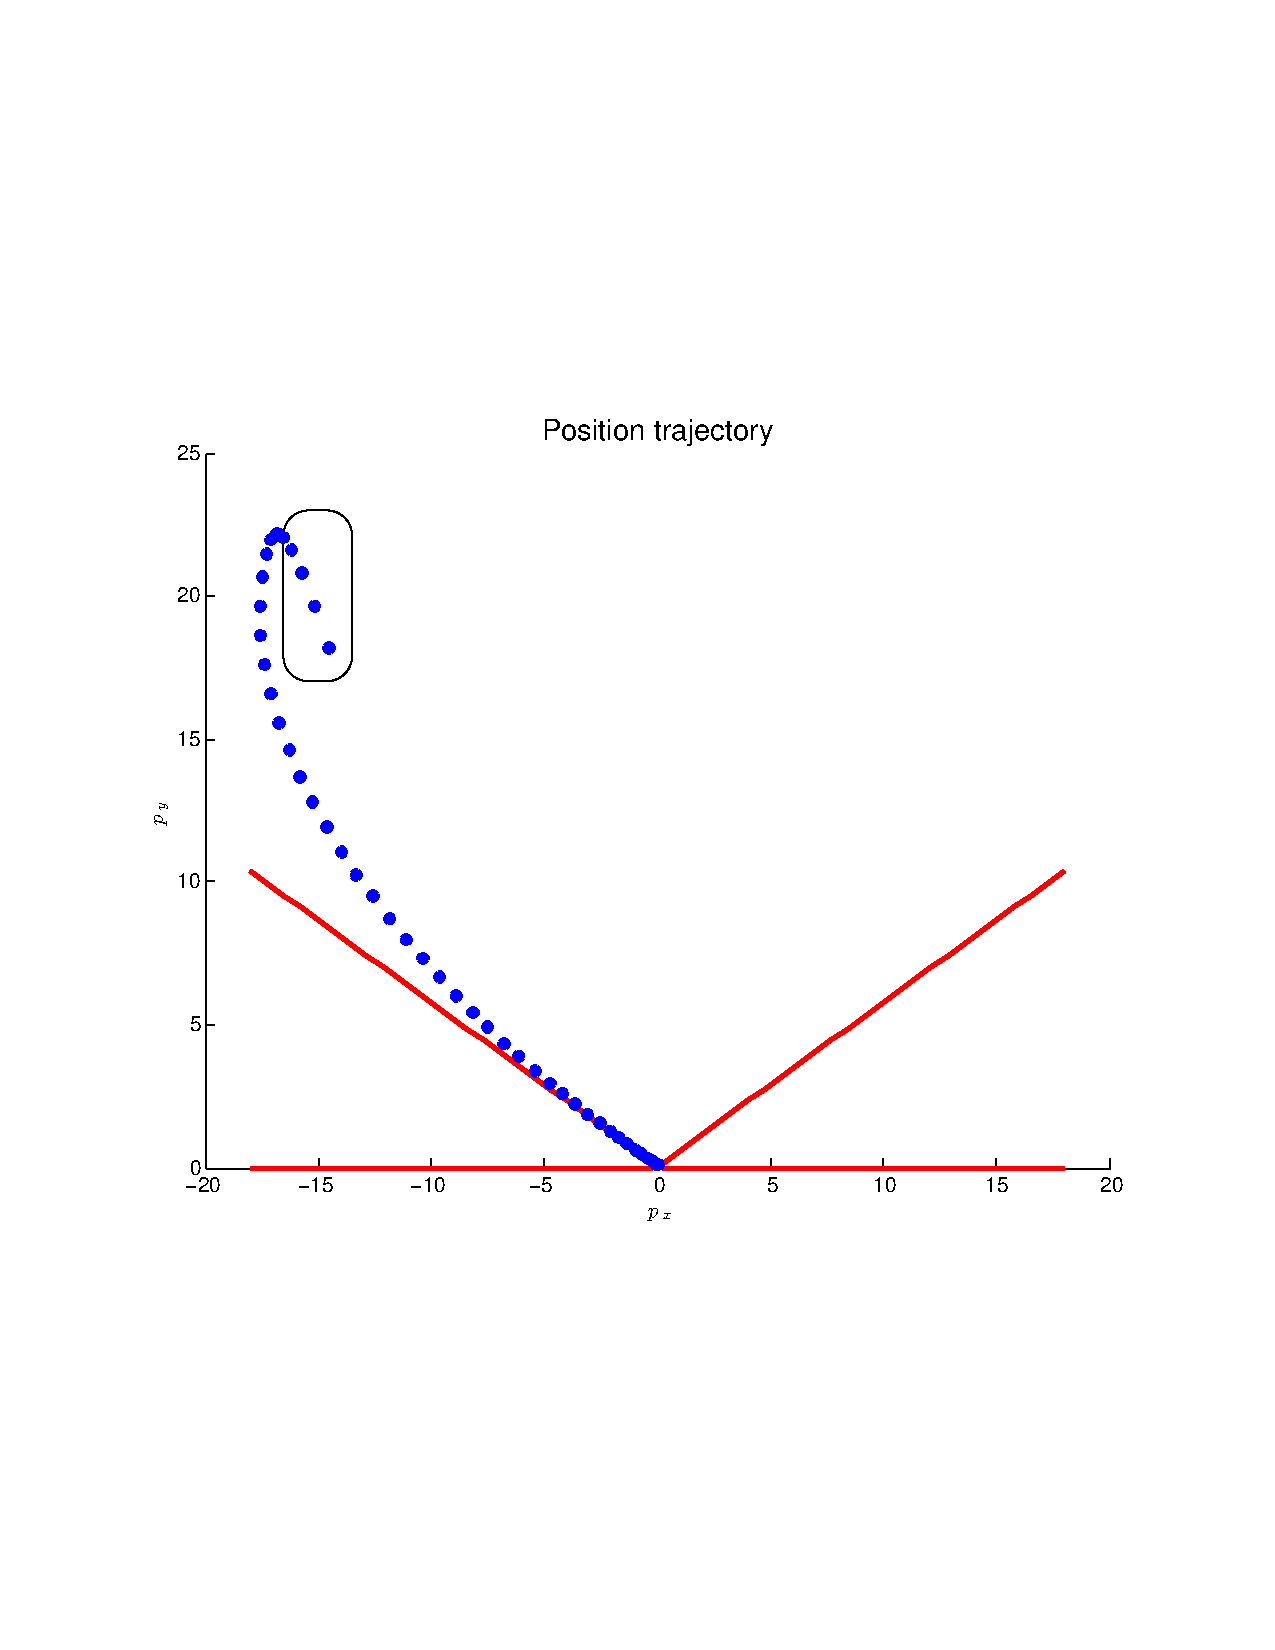
\includegraphics[width=\textwidth]{Figures/states}
                \caption{$x-y$ coordinates of spacecraft}
                \label{fig:soft-landing-state}
        \end{subfigure}%
        ~ %add desired spacing between images, e. g. ~, \quad, \qquad, \hfill etc.
          %(or a blank line to force the subfigure onto a new line)
        \begin{subfigure}[b]{0.5\textwidth}
                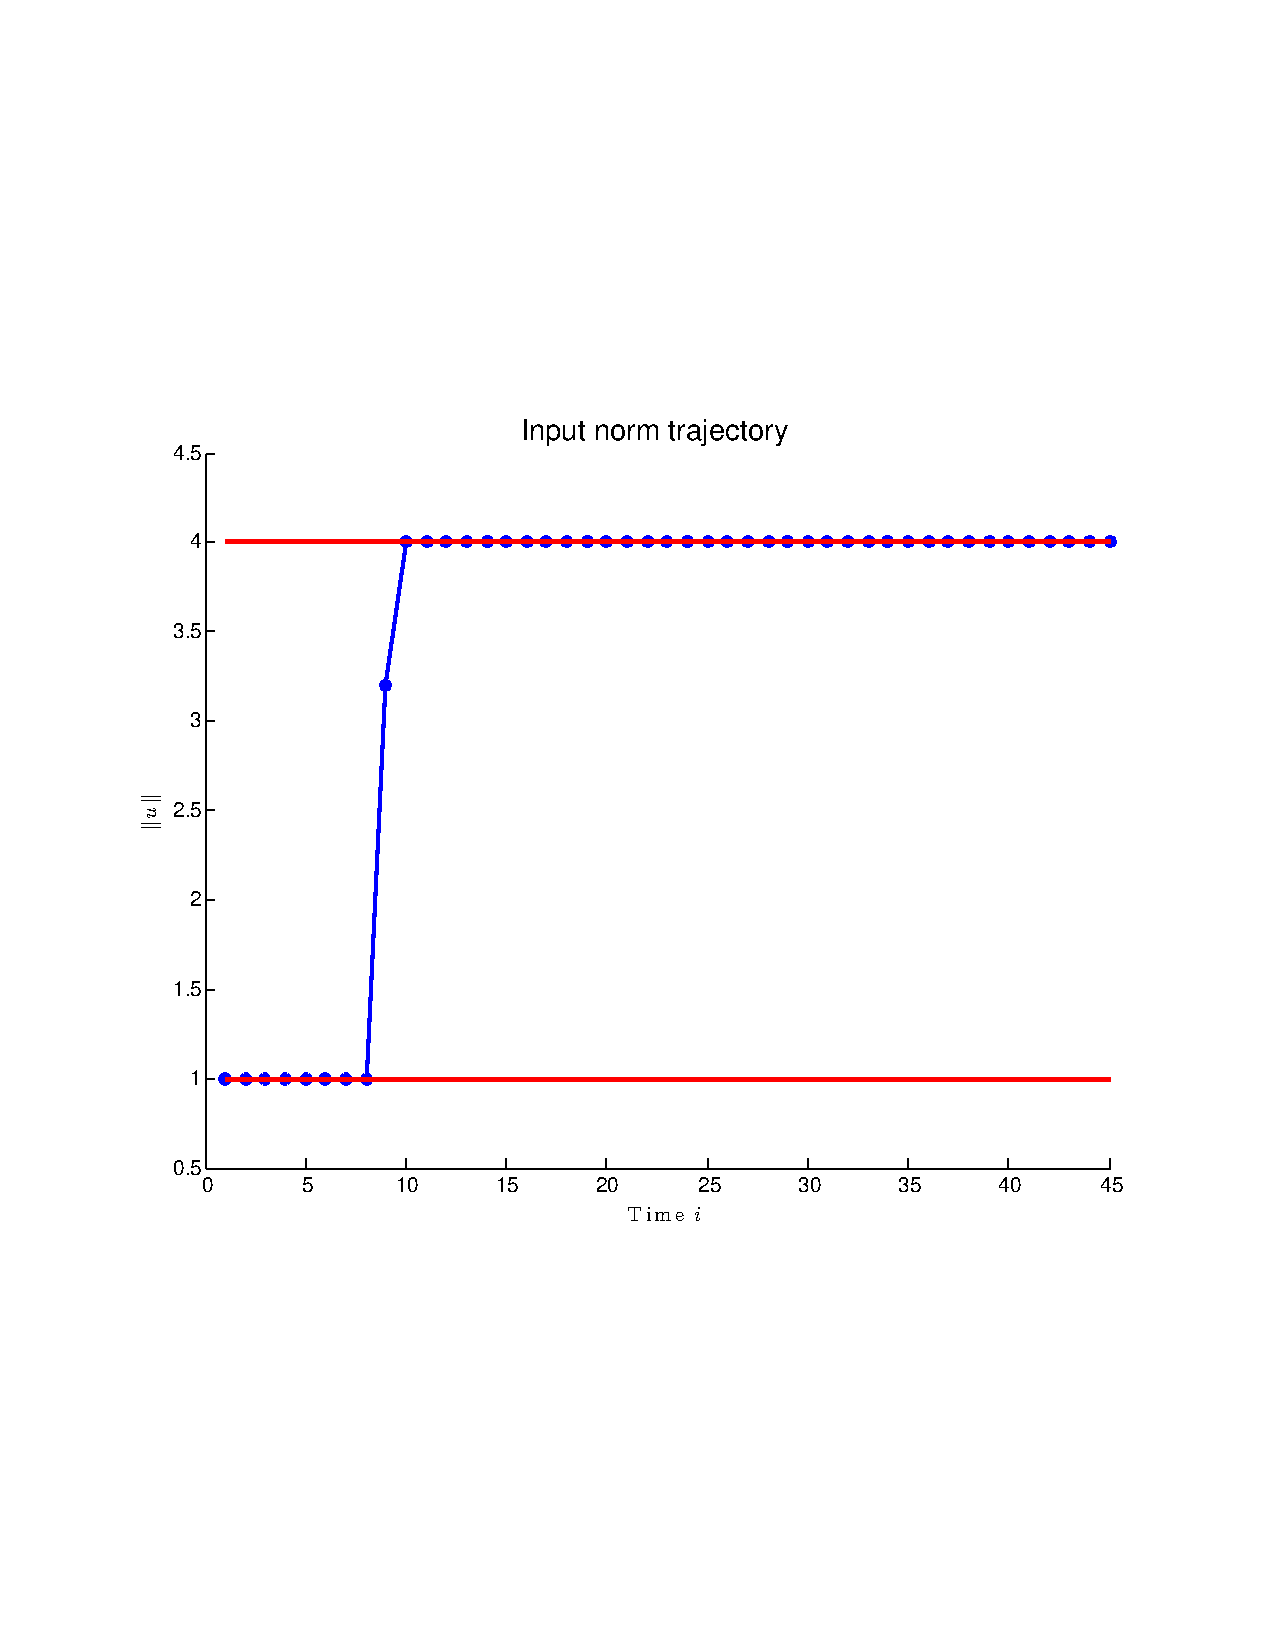
\includegraphics[width=\textwidth]{Figures/inputs}
                \caption{Norm of inputs}
                \label{fig:soft-landing-inputs}
        \end{subfigure}%
        ~ %add desired spacing between images, e. g. ~, \quad, \qquad, \hfill etc.
          %(or a blank line to force the subfigure onto a new line)
        \caption{Trajectory of the position as the spacecraft lands to the specified point $z_f=(0,0.1)$. The initial state lies within some interval away from the desired one $z_0=(-15,20)$. With red color is depicted the glide angle constraint. Observe that many state constraints are active at the optimal trajectory. In the second plot the optimal input trajectory is depicted. As expected, the convex relaxation is exact, \ie, the inputs stay in between 1 and 4. Note that almost all of them are saturated at optimality.}\label{fig:animals}
\end{figure}


\section{Building economic control}\label{SEC:example}
In this section, we consider a control problem for a building heating system and design an MPC controller to minimize the total cost of operation that takes into account the prediction of the weather. The heating system is modeled by a discrete linear system 
%
\begin{align*}
x_{i+1} &=Ax_i+Bu_i+Bd_i \\
y_i &=Cx_i\enspace.
\end{align*}
%
The system has ten states in $x_t$ without specific physical interpretation. The system input $u_t = (u_1, u_2, u_3)$ includes the electrical power input (kW) to the heating system of the three zones. The disturbance input $d_t = (d_1, d_2, d_3)$ constitutes the outside temperature ($\,^{\circ}\mathrm{C}$), solar gains (kW), and internal gains (kW). The output of the system $y_t = (y_1, y_2, y_3)$ represents the temperature in the three building zones. There are ten states in the model, however they do not have any physical interpretation.XXX The sampling rate of the system is $T_s = 20$ min. 

The purpose is to design an economic MPC controller with the objective is to keep the temperature of the building zones within the comfort constraints, while minimizing the energy bill. The economic MPC controller uses an economic linear cost function in Problem~\ref{pr: Economic MPC controller}, as opposed to the usual quadratic cost function used in regulation problems. The inputs and the outputs of the model are subject to box-constraints.

\begin{equation}\label{pr: Economic MPC controller}
  \begin{array}{ll}
        \mbox{minimize} & \sum^{N}_{i=0} c^{T}_{i}u_{i}  \\
    \mbox{subject to} & x_{i+1} = Ax_i+B_uu_i+B_dd_i, \; i = 0,\ldots,N-1 \\
    \quad & y_i = C x_i, \\
  \quad & u_{min} \leq u_i \leq u_{max} \; i = 0,\ldots,N-1 \\
  \quad & y_{min} \leq y_i \leq y_{max}, \; i = 1,\ldots,N\enspace,
  \end{array}
\end{equation}

The input constraints capture the heating capacity of the building system with $u_{min} = 0\; kW$ and $u_{max} = 15\; kW$, while the output constraints ensure comfort in the building with $y_{min} = 22 \,^{\circ}\mathrm{C}$ and $y_{max} = 26 \,^{\circ}\mathrm{C}$. The sequence $d_i$ denotes the disturbance prediction, and $c_i$ is the electricity prices with a periodic high price and low price periods, i.e., $c_i=0.04\; \$/kWh$ (between 00:00Hrs to 10:00Hrs, and 16:00Hrs to 24:00Hrs) and $c_i=0.2\; \$/kWh$ (between 10:00Hrs to 16:00Hrs). The economic MPC problem can be formulated as a linear programming problem.

\chapter{Summary}{\label{ch:splitGuideline}}
The first question that comes to mind when making use of a splitting method is how to perform the splitting. This choice can heavily affect the speed of the algorithm. Choosing a splitting pattern is equivalent to formulating the $M+1$ subproblems that have to be solved in the three algorithmic schemes. Consequently, the choice will also confine the options for acceleration and preconditioning. A general guideline would be the following:
\begin{enumerate}
\item All subproblems should have a closed form solution if possible; if not, they should be cheap to solve. The whole purpose of using splitting on (\ref{eq:format}) is to end up with simpler subproblems. 
\end{enumerate}
All the acceleration techniques discussed in Chapters~\ref{ch:acceleration} and~\ref{ch:speedup} can be practically seen as ways to robustify the algorithms against the stepsize parameter and the conditioning of the data. Note that, for a given set of data, there ideally exist theoretically optimal stepsize and relaxation constants. Due to the fact that these constants cannot be computed in most of the cases, we reduce the dependence on those by means of several heuristics. More specifically, we have observed that: 
\begin{enumerate}[resume]
\item Preconditioning should always be used if possible. It has been empirically observed that it is the most decisive factor for speeding up convergence.
\item Adaptation of the stepsize, especially in ADMM, can speedup convergence dramatically. In the case that simultaneous diagonalization can be used (see Chapter~\ref{ch:speedup2}), adaptation should be used. Even if simultaneous diagonalization is not possible, it might be worth solving the first of a series of problems with adaptive stepsize strategy, despite the increased cost per iteration. The resulting stepsize (upon convergence) can then be used as a fixed one in the subsequent problems as the horizon recedes. It is observed that, even in the case that the optimal stepsize is known, adaptation might further reduce the number of iterations. 
\item If an accelerated version of an algorithm can be used without heavily altering a well-structured problem, then it should be used. Acceleration generally improves significantly the number of iterations needed for convergence. Restarting of the scheme is optional in the case of AMA. Although restarting can end up increasing the number of iterations needed for convergence, in our experience it generally acts beneficially on the method. In both ADMM and AMA, the combination of the accelerated (restarted) versions with an adaptive stepsize strategy works well in practice. For FPDA the adaptation is already embedded in Step~4 of the method. 
\end{enumerate}
In many cases the approaches described above are competing. For example, one can precondition the problem so that an accelerated variant of a method can be used, but at the same time some favorable sparsity pattern of the original problem is lost.
In our experience, there is no `golden rule' when it comes to choosing a particular method and applying the various extensions for speeding it up. The choice of the method should be motivated from the problem's structure and vice-versa. In the subsequent Figures~\ref{fig:flowChartAMA}, \ref{fig:flowChartPDA} and \ref{fig:flowChartADMM} we attempt to give a rough guideline on how an algorithm should be modified, once selected. The flow chart should be conceived as a proposed sequence of steps, in the sense that they usually (but not necessarily) enhance the performance of the algorithm. The steps suggested are also allowable, in the sense that \emph{convergence guarantees are ensured and the computational cost is not significantly increased}.


Warm-starting\\
Linear programs, ADMM for non-quadratics\\
Regarding the choice of the algorithm, there is typically a tradeoff between expensive operations and number of iterations. This tradeoff has to be evaluated on the specific application. For example, time-critical applications might tolerate an increased computational cost per iteration in order to achieve a (relatively) accurate solution in less iterations. Resource-limited applications might, on the other hand, prefer lighter computations at the expense of more iterations for convergence. It is difficult, however, to know in advance which of the two approaches will take less time. A good indicator is the average number of flops, \ie, the number of operations per iteration multiplied by the average number of iterations for each algorithm. 

Below, we examine each method separately, in more detail.\\

\begin{figure}
        \centering
        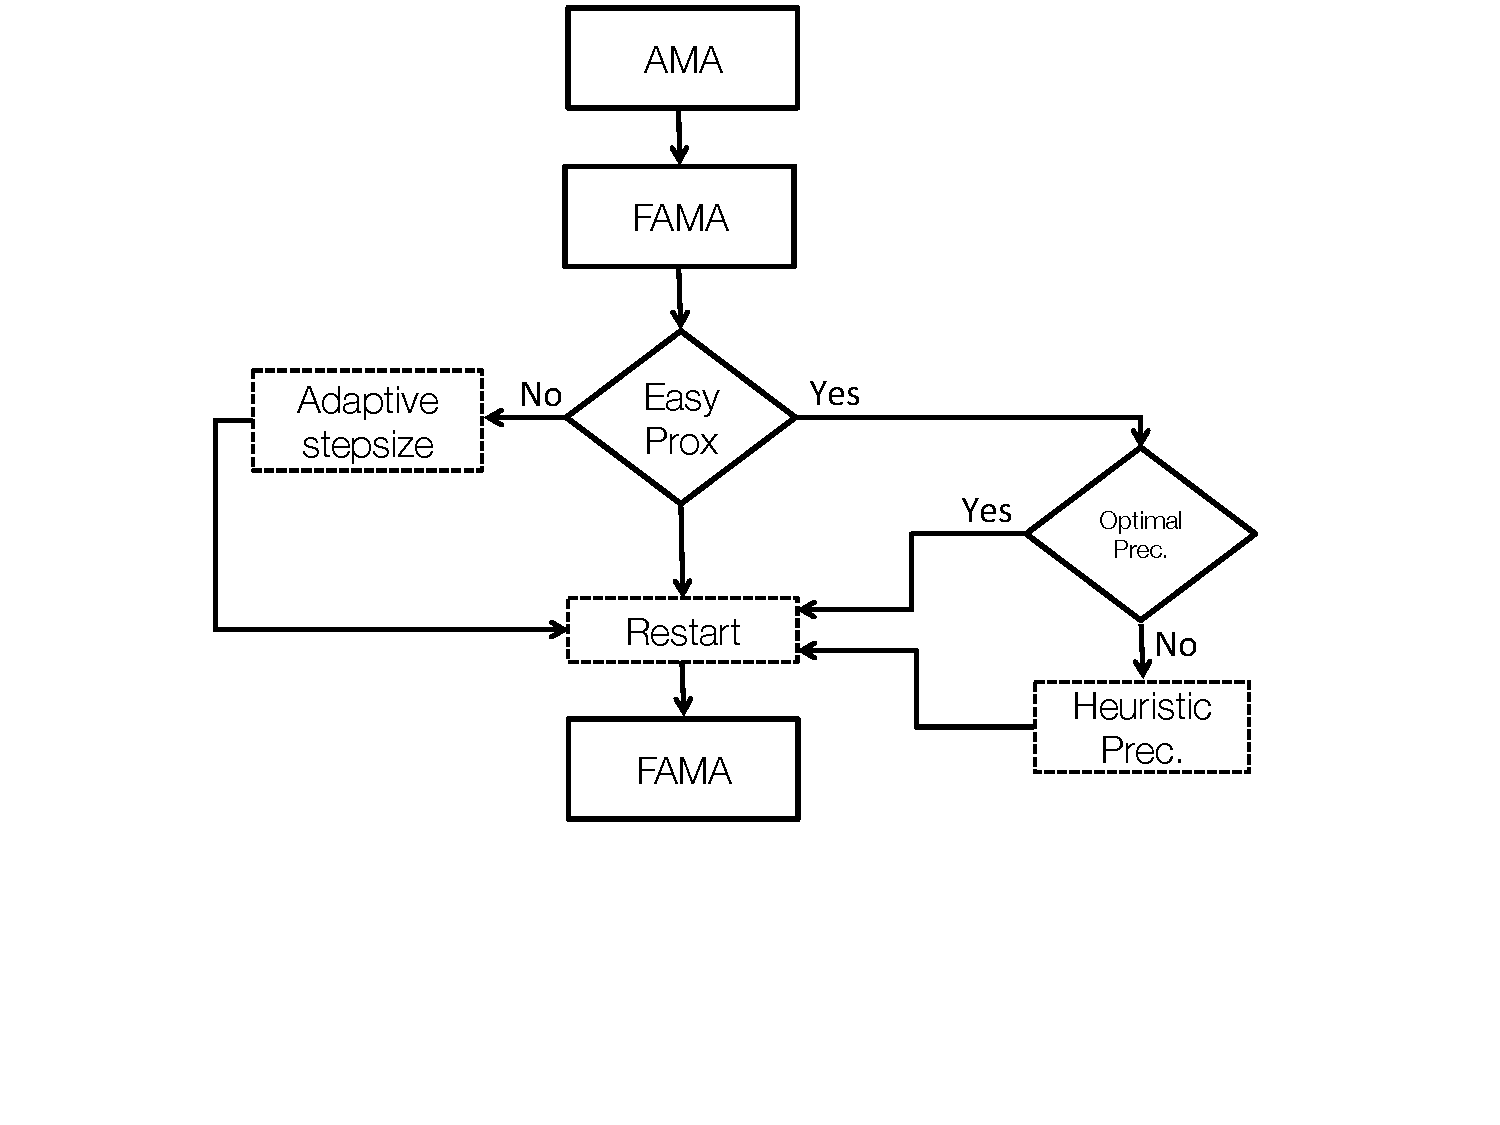
\includegraphics[width=75mm,scale=0.75]{Figures/FlowChartAMA}
        \caption{Flow chart for AMA. }
        \label{fig:flowChartAMA}
\end{figure}
\begin{figure}
        \centering
        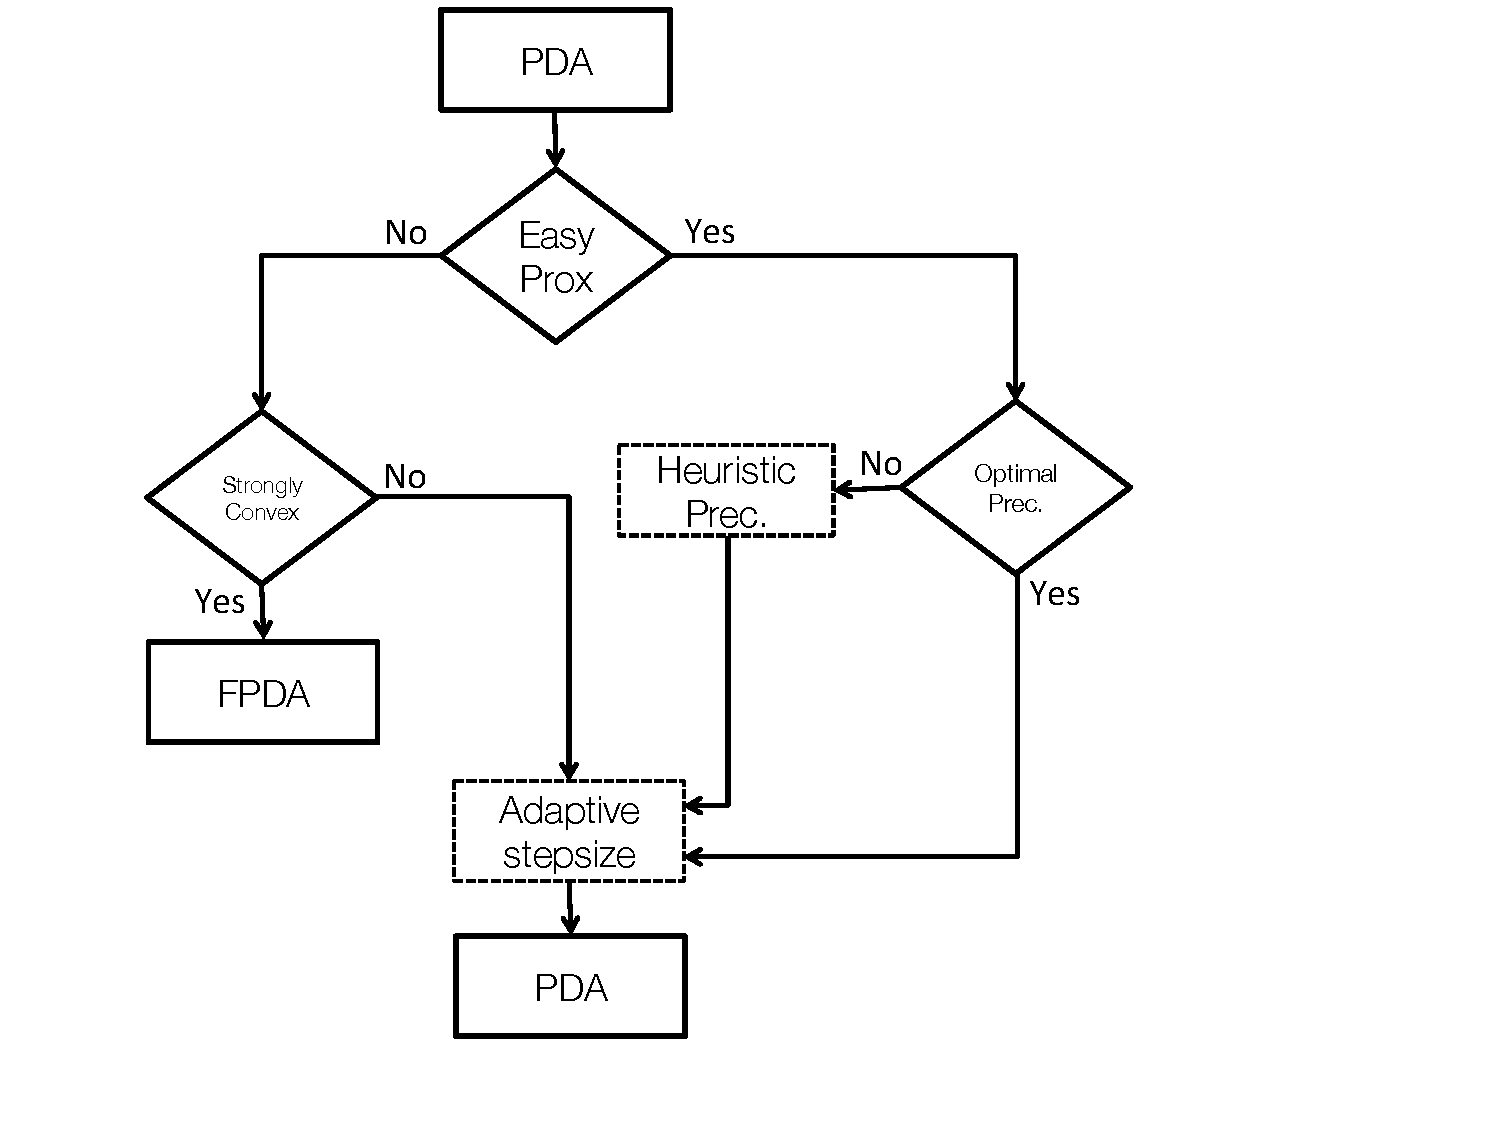
\includegraphics[width=75mm,scale=0.75]{Figures/FlowChartPDA}
        \caption{Flow chart for PDA. }
        \label{fig:flowChartPDA}
\end{figure}
\begin{figure}
        \centering
        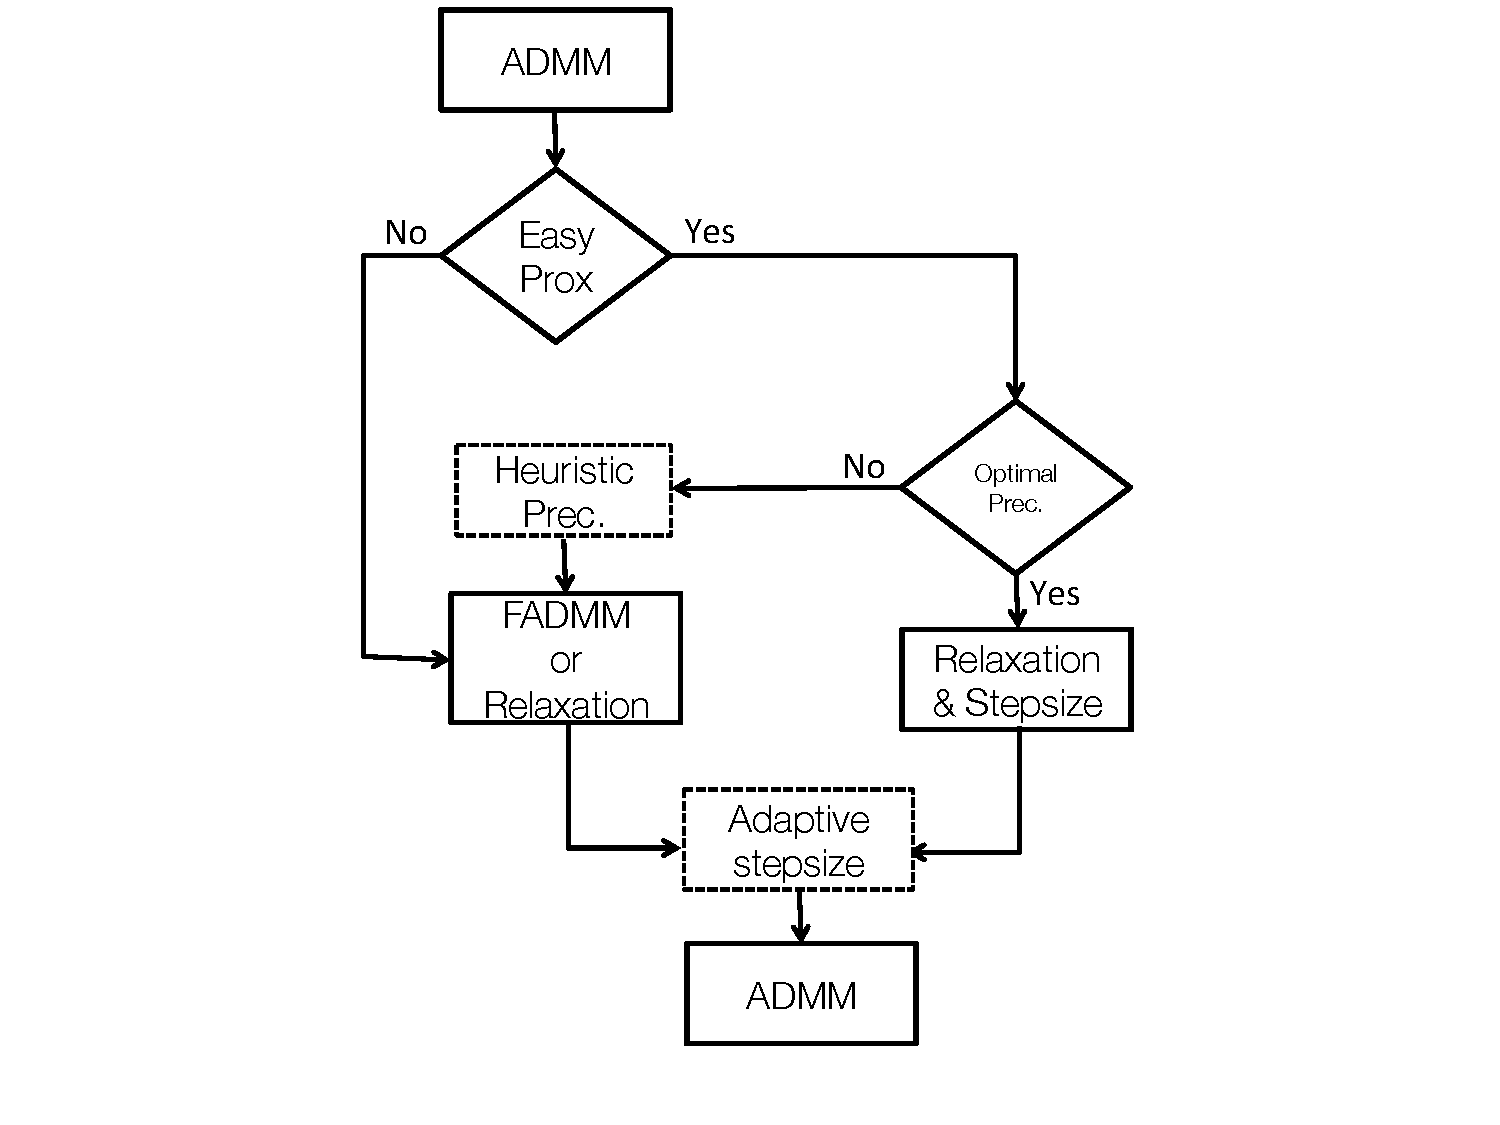
\includegraphics[width=75mm,scale=0.75]{Figures/FlowChartADMM}
        \caption{Flow chart for ADMM. }
        \label{fig:flowChartADMM}
\end{figure}



\appendix


\chapter{Definitions}{\label{App::Definitions}}
In this Appendix we give several definitions of notions that appear throughout the survey.

\paragraph{Subdifferential and Conjugacy}
\definition (Subdifferential): The subdifferential of a convex function $f$ at $x$ is defined as 
\[
\partial f(x)=\{u : \langle u,z-x\rangle\le f(z)-f(x)\;\forall z \in \dom f\}.
\]
Note that when $f$ is differentiable, $\partial f(x)=\{\nabla f(x)\}$.

\definition (Conjugate): The conjugate of a convex function $f:\reals^n\to\overline{\reals}$, denoted by $f^\star:\reals^n\to\overline{\reals}$, is defined as 
\[
f^\star(\lambda)=\underset{z}{\sup}\left\{\langle z,\lambda\rangle-f(z)\right\}\enspace.
\]
\begin{theorem}{\label{App:conj_subd}}
Let $f\in\Gamma_0(\reals^n)$. The following relation holds:
\begin{equation*}
u\in\partial f(x), \mbox{ for some } x\in\reals^n, \; \Leftrightarrow \; x\in\partial f^\star(u)\enspace.
\end{equation*}
\end{theorem}

The notion of the conjugate function is quite useful in the framework of first-order methods for convex optimization.
Below, we give some pairs of conjugate functions that we usually meet in the problems of interest.
\begin{center}
    \begin{tabular}{ | l | c | c | }
    \hline
     Description & $f(z)$ & $f^{\star}(\lambda)$ \\ \hline\hline
     Nonnegative orthant & $\delta_+(z)$ & $\delta_-(\lambda)$ \\ \hline
     Box/$l_\infty$-norm ball ($\|z\|_{\infty}\leq l$) & $\delta_{\infty}(z,l)$ & $l\|\lambda\|_1$ \\ \hline
     $l_1$-norm ball ($\sum_i |z_i|\leq l$)  & $\delta_1(z,l)$ & $l\|\lambda\|_{\infty}$ \\ \hline
     $l_2$-norm ball ($\|z\|_2\leq l$)  & $\delta_2(z,l)$ & $l\|\lambda\|_2$ \\ \hline
     Lorentz cone ($\|z\|_2\leq t$, $(z,t)\in \reals^{n+1}$) & $\delta_2(z,t)$ & $\delta_2(\lambda,y)$ \\ \hline
     %Quadratic & $(1/2)x^TQx + r^Tx + s$ & $(1/2)p^TQ^{-1}p - \langle p,Q^{-1}r\rangle  + (1/2)\langle r,Q^{-1}r\rangle  - s$ \\ \hline
    \end{tabular}
    {\label{table:conjugacy}}
\end{center}
Table~\ref{table:conjugacy} by no means covers the wide spectrum of convex conjugate functions that can be analytically derived. We refer the interested reader to the work~\cite{combettes2011proximal} for an exhaustive list of conjugate functions. Similarly, since proximal operators of convex functions have been derived in numerous works, we do not intend to list them here. We once more refer the interested reader to~\cite{combettes2011proximal} for a list, as well as~\cite{parikh2014proximal} for the derivation procedure of the most common ones. Finally, the Matlab library~\cite{proxMatlab} implements many proximal operators for direct use, serving as a supplement to~\cite{parikh2014proximal}. 

\paragraph{Structural properties}
\definition (Smoothness): A function $f\in\Gamma_0(\reals^n)$ is $\beta$-smooth if it is differentiable and
\[
 f(z) \le f(x) + \langle \nabla f(x), z-x\rangle + (\beta/2)\|z-x\|^2\enspace,
\]
holds for all $z,x\in\reals^n$.

 \definition (Strong convexity): A function $f\in\Gamma_0(\reals^n)$ is $\beta$-strongly convex if
\[
 f(z) \ge f(x) + \langle u, z-x\rangle + (\beta/2)\|z-x\|^2\enspace,
\]
holds for all $z,x\in\reals^n$ and all $u\in\partial f(x)$.

\remark The above definitions generalize in the case of positive semi-definite matrices $P\in\psd_+$ instead of scalars $\beta$. The inequalities then hold with $(1/2)\|z-x\|^2_P$.

\definition (Lipschitz continuous gradient): A differentiable function $f\in\Gamma_0(\reals^n)$ has a $\beta$-Lipschitz continuous gradient if
\[
 \|\nabla f(z) - \nabla f(x)\| \le \beta\|z-x\|\enspace.
\]
$\beta$-Lipschitz continuous gradient is equivalent to $\beta$-smoothness of the function.

\begin{lemma}{\label{App:BH}}
Let $f\in\Gamma_0(\reals^n)$. The following statements are equivalent:\\
The function $f$ is $\beta$-strongly convex function.\\
The conjugate function $f^\star\in\Gamma_0(\reals^n)$ has $1/\beta$-Lipschitz continuous gradient.
\end{lemma}

\begin{remark}
 All the definitions and lemmata given above hold for $\dom f=\mathcal{Z}\subseteq\reals^n$. We choose to restrict ourselves to $\dom f=\reals^n$ for simplicity. In this manuscript, when the domain of a function is a subset of the real numbers, this is explicitly treated via indicator functions.
\end{remark}

\paragraph{Useful identities}

Moreau identity is a very useful Lemma that associates a convex function with its conjugate. This is instrumental for deriving all the algorithms presented in this work, since, as we saw, their derivation depends on the application of proximal methods to the dual function~\eqref{eq:dual}, which is expressed via conjugate functions. Below we give Moreau identity associated to the proximal, as well as the generalized proximal operator~\eqref{eq::genProx}.
\begin{lemma}{\label{App.:Moreau}}
 Let $f\in \Gamma_0(\reals^n)$. Then for any $x\in\reals^n$
 \[
  \prox{_{\rho f^{\star}}}(x) + \rho \prox{_{f/\rho}}(x/\rho) = x, \;\; \forall\; 0 < \rho < +\infty\enspace.
 \]
\end{lemma}

\begin{lemma}{\label{App.:genMoreau}}
 Let $f\in \Gamma_0(\reals^n)$ and $P\in\psd_{++}$. Then for any $x\in\reals^n$
 \[
  \prox{_{\rho f}^{P}}(x) + \rho P^{-1}\prox{_{f/\rho}^{P^{-1}}}(P(x/\rho)) = x, \;\; \forall\; 0 < \rho < +\infty\enspace.
 \]
\end{lemma}


\iffalse
\section{Fenchel conjugate of second order cone}
In what follows we derive the convex conjugate of a second order cone constraint. Consider the optimization problem
    \begin{equation}   
    \begin{array}{ll}
      \mbox{minimize} & 0 \\
      \mbox{subject to} & \|Ax+b\|_2 \le c^Tx+d\enspace,
    \end{array}
    \end{equation}
which can be reformulated as
    \begin{equation}{\label{App:SOC_prim}}
    \begin{array}{ll}
      \mbox{minimize} & I_2(v,t) \\
      \mbox{subject to} & v = Ax+b \\
                \quad & t = c^Tx+d \enspace.
    \end{array}
    \end{equation}
The Lagrangian formulation for (\ref{App:SOC_prim}) is
\begin{align}
L \nonumber&= \underset{\lambda_1,\lambda_2}{\max} \; \underset{x,v,t}{\min} \Big\{I_2(v,t) + \langle \lambda_1,v-Ax-b\rangle  + \lambda_2(t-c^Tx-d)\Big\}\\
  &= \underset{\lambda_1,\lambda_2}{\max} \Big\{ \underset{x}{\min} \{-\langle \left[\begin{array}{c}Ax+b\\c^Tx+d\end{array}\right],\left[\begin{array}{c}\lambda_1\\\lambda_2\end{array}\right]\rangle \} + \underset{v,t}{\min} \{ \langle \left[\begin{array}{c}v\\t\end{array}\right],\left[\begin{array}{c}\lambda_1\\\lambda_2\end{array}\right]\rangle  + I_2(v,t)\}\Big\}{\label{App:lagrang}}
\end{align}
Let us focus on solving for the second part of (\ref{App:lagrang}). We have that
\begin{align*}
 &\underset{v,t}{\min} \{ \langle \left[\begin{array}{c}v\\t\end{array}\right],\left[\begin{array}{c}\lambda_1\\\lambda_2\end{array}\right]\rangle  + I_2(v,t)\}\\
 &=-\underset{\|v\|_2\le t}{\max} \{ -\lambda_1^Tv-\lambda_2 t \}\enspace.
\end{align*}
From Cauchy-Schwarz it holds that
\begin{align}
  \underset{\|v\|_2\le t}{\max} \{ -\lambda_1^Tv-\lambda_2 t \} &\le \underset{t\ge 0}{\max} \{ \|\lambda_1\|_2\|v\|_2-\lambda_2 t \}\\
                                                                &\le \underset{t\ge 0}{\max} \{ t(\|\lambda_1\|_2-\lambda_2) \}\\
                                                                & = I_2(\lambda_1,\lambda_2) = \left\{ \begin{array}{ll} 0 & \|\lambda_1\|\le\lambda_2 \\
                                                                                                                    \infty & \mbox{otherwise}.
                                                                                                      \end{array} \right.
\end{align}
Finally, problem (\ref{App:SOC_prim}) can be written as
\begin{equation}
\underset{x}{\min}\;\underset{\lambda_1,\lambda_2}{\max} \Big\{-\langle \left[\begin{array}{c}Ax+b\\c^Tx+d\end{array}\right],\left[\begin{array}{c}\lambda_1\\\lambda_2\end{array}\right]\rangle  - I_2(\lambda_1,\lambda_2)\Big\}\enspace.
\end{equation}
\fi



\chapter{Derivation of the algorithms from proximal methods}{\label{App::AlgsDerivations}}
The subsequent results are instrumental as they demonstrate the equivalence of the AMA, PDA and ADMM to proximal algorithmic schemes, as presented in Chapter~\ref{ch:algorithms}, when applied to the dual problem~\eqref{eq:dual}. We repeat here the dual function for clarity:
\begin{equation*}   
  -d(\lambda) =  F(\lambda) + g^\star(\lambda)\enspace,
\end{equation*}
where $F(\lambda):=f^\star(-L^T\lambda) - \langle  \lambda,l\rangle $.

\paragraph{AMA and PGM.}
The Alternating Minimization Algorithm can be derived from the application of the PGM iteration~\eqref{ch2::eq:PGM} to $-d$. The proof is inspired from \cite[Lemma~3.2]{beck2014fast}, where the equivalence between the accelerated versions of AMA and PGM is drawn.

Since $f$ is strongly convex, it follows from Lemma~\ref{App:BH} that $f^\star$ is smooth. Subsequently, $F$ is also smooth. Then $\nabla F$ is Lipschitz continuous with some constant $L_F$, and the proximal gradient algorithm reads
\begin{algorithm}[H]
\caption{Dual Proximal Gradient Method}
\label{al:PGM}
\begin{algorithmic} 
\REQUIRE Initialize $\rho < 2/L_F$.
\LOOP
\STATE 1: $z^{k+1} = \argmin\limits_z \quad f(z) + \langle  L^T\lambda^k, z\rangle $
\STATE 2: $\lambda_i^{k+1} = \prox_{\rho g_i^\star}\left(\lambda_i^k+\rho(L_iz^{k+1}+l_i)\right), \; i=1,\ldots,M$
\ENDLOOP
\end{algorithmic}
\end{algorithm}\begin{footnotesize}
\end{footnotesize}

The following Lemma holds:
\begin{lemma}{\label{App.:AMA_PGM}}
The second step of Algorithm~\ref{al:PGM}
is equivalent to steps 2 and 3 of Algorithm~\ref{al:AMA} combined, written as
\begin{align*}
 y_i^{k+1} &= \prox{_{g_i/\rho}}\left(L_iz^{k+1}+l_i+\lambda_i^k/\rho\right)\\
 \lambda_i^{k+1} &= \lambda_i^k + \rho(L_i z^{k+1} +l_i- y_i^{k+1})\enspace.
\end{align*}
\end{lemma}

\begin{proof}
Step~1 of Algorithm~\ref{al:PGM} amounts to computing the gradient of $f^\star(-L^T\lambda)-\langle  \lambda,l\rangle $. Using Theorem~\ref{App:conj_subd}, 
\begin{equation*}
  -L^T\lambda^k \in \partial f(z^{k+1}) \Leftrightarrow z^{k+1} = \nabla f^\star(-L^T\lambda^k)\enspace.
\end{equation*}
Thus, the gradient of $F$ can be expressed as
\[
\nabla F(\lambda^k) = -Lz^{k+1} - l\enspace.
\]
Step~2 is, apparently, the proximal step with respect to $g^\star_i$ in the direction of the negative gradient.

We are now ready to prove the assertion. To this end, we first denote $\mu_i^k=\lambda_i^k + \rho(L_i z^{k+1}+l_i)$, and subsequently substitute the result of the proximal step $y_i^{k+1}$ to the dual update $\lambda_i^{k+1}$\enspace:
\begin{align*}
 \lambda_i^{k+1} &= \lambda_i^k + \rho(L_i z^{k+1}+l_i) - \rho\prox{_{g_i/\rho}}(\lambda_i^k/\rho + L_i z^{k+1}+l_i) \\
                 &= \mu_i^k- \rho\prox{_{g_i/\rho}}(\mu_i^k/\rho)\enspace.
\end{align*}

Using Moreau identity (\ref{App.:Moreau}), it directly follows that
\begin{equation*}
 \lambda_i^{k+1} = \mu_i^k- \mu_i^k+ \prox{_{\rho g^\star_i}}(\mu_i^k) = \prox{_{\rho g_i^\star}}(\mu_i^k)\enspace.
\end{equation*}
\end{proof}

Finally, the accelerated version of PGM, named \emph{Fast Proximal Gradient Method (FPGM)}~\cite{beck2014fast},\cite{Giselsson:fbds}, applied to the dual problem, is given below. The method is the result of simply applying Nesterov's momentum scheme to Algorithm~\ref{al:PGM}, as discussed in Chapter~\ref{ch:acceleration}. Any other acceleration sequence~\cite{tseng2008accelerated} would result to similar algorithms.
\begin{algorithm}[H]
\caption{Fast Dual Proximal Gradient Method}
\label{al:FPGM}
\begin{algorithmic} 
\REQUIRE Initialize $\rho \in (0,1/L_F]$, $\lambda^{-1}=\lambda^{0}\in\reals^p$, $\alpha^{-1}=\alpha^{0}=1$.
\LOOP
\STATE 1: $\hat{\lambda}^{k} = \lambda^{k}+((\alpha^{k-1}-1)/\alpha^k)(\lambda^k-\lambda^{k-1})$
\STATE 2: $z^{k} = \argmin\limits_z \quad f(z) + \langle  L^T\hat{\lambda}^k, z\rangle $
\STATE 3: $\lambda_i^{k+1} = \prox_{\rho g_i^\star}\left(\hat{\lambda}_i^k+\rho(L_iz^{k}+l_i)\right), \; i=1,\ldots,M$
\ENDLOOP
\end{algorithmic}
\end{algorithm}\begin{footnotesize}
\end{footnotesize}

\paragraph{PDA and PGM.} 
Consider the problem~\eqref{eq:format} that can be written as
\begin{equation*}
     \begin{array}{ll}
      \mbox{minimize} & h(z)+\delta_\mathcal{D}(z)+g(Lz+l)\enspace,
    \end{array}
\end{equation*}
with $h(z)$, $\delta_\mathcal{D}(z)$ as defined in~\eqref{eq:split_f}. 
We now consider the quadratic approximation of $h(z)$ expressed as:
\[
 \hat{h}(z) = h(x) + \langle\nabla h(x),z-x\rangle + (1/2\tau)\|z-x\|_2^2\enspace, 
\]
for all $z,x\in\reals^n$ and $\tau>0$.
We have the following relations:
\begin{align*}
 &\underset{z}{\min} \left\{ h(x) + \langle\nabla h(x),z-x\rangle + (1/2\tau)\|z-x\|_2^2+\delta_\mathcal{D}(z)+g(Lz+l)\right\} = \\
 &\underset{\lambda}{\max}\;\underset{z,y}{\min} \left\{ h(x) + \langle\nabla h(x),z-x\rangle + (1/2\tau)\|z-x\|_2^2+\delta_\mathcal{D}(z)+g(y)+\langle\lambda,Lz+l-y\rangle\right\}=\\
 &\underset{\lambda}{\max}\;\underset{z}{\min}\;-\underset{y}{\max} \left\{\delta_\mathcal{D}(z)+(1/2\tau)\|z-(\underbrace{x-\tau\nabla h(x)}_{v})\|_2^2+\langle\lambda,Lz+l+y\rangle-g(y)\right\}=\\
 &\underset{\lambda}{\max}\;\underset{z}{\min} \left\{\delta_\mathcal{D}(z)+(1/2\tau)\|z-v\|_2^2+\langle\lambda,Lz+l\rangle+g^\star(\lambda)\right\}=\\
 &\underset{\lambda}{\max}\;\underset{z}{\min} \left\{\delta_\mathcal{D}^r(z)+\langle L^T\lambda,z\rangle+\langle \lambda,l\rangle+g^\star(\lambda)\right\}=\\
 &\underset{\lambda}{\min} \left\{\left(\delta_\mathcal{D}^r\right)^\star(-L^T\lambda)-\langle l,\lambda\rangle+g^\star(\lambda)\right\}\enspace,
\end{align*}
where we denoted the \emph{regularized} dynamics indicator function as
\[
 \delta_\mathcal{D}^r(z) := \delta_\mathcal{D}(z) + (1/2\tau)\|z-x\|_2^2\enspace.
\]
Note that $\delta_\mathcal{D}^r$ is strongly convex, hence $\left(\delta_\mathcal{D}^r\right)^\star$ is smooth. So we can apply the PGM to $-\hat{d}(\lambda):=\left(\delta_\mathcal{D}^r\right)^\star(-L^T\lambda)-\langle l,\lambda\rangle+g^\star(\lambda)$. We can now follow the same reasoning as in the case of AMA.

Consider $x=z^k$ and $v^k=z^k-\tau\nabla h(z^k)$. Denote also the smooth part of $\hat{d}(\lambda)$ as $\hat{F}(\lambda)=\left(\delta_\mathcal{D}^r\right)^\star(-L^T\lambda)-\langle l,\lambda\rangle$. Step~1 of Algorithm~\ref{al:PDA} can be expressed as
\begin{align*}
 z^{k+1} &= \underset{z}{\argmin}\left\{\delta_\mathcal{D}(z) + (1/2\tau)\|z-v^k\|_2^2 + \langle\lambda^k,Lz+l\rangle\right\}\\
         &=\underset{z}{\argmin}\left\{\delta_\mathcal{D}^r(z)+ \langle\lambda^k,Lz+l\rangle\right\}.
\end{align*}
The optimality condition reads
\begin{align}
 \nonumber& -L^T\lambda^k \in \partial \delta_\mathcal{D}^r(z^{k+1}) \\
 \nonumber &z^{k+1} = \nabla\left(\delta_\mathcal{D}^r\right)^\star(-L^T\lambda){\label{App::eq:optCondPDA}}\enspace.
\end{align}
Consequently, the gradient of $\hat{F}(\lambda)$ is 
\[
 \nabla \hat{F}(\lambda) = -L\nabla\left(\delta_\mathcal{D}^r\right)^\star(-L^T\lambda)=-Lz^{k+1}-l.
\]
Finally, the proximal update of Algorithm~\ref{al:PGM} coincides with Step~2 of Algorithm~\ref{al:PDA}, evaluated at the over-relaxed point $2z^{k+1}-z^k$. However, note that the convergence condition imposed on the stepsizes is not the same, \ie, PDA needs $\sqrt{\tau\rho}<\frac{(1-\tau L_h/2)}{\sqrt{\sum_{i=1}^{M}\|L_i\|^2}}$. This condition already poses the restriction that $\tau<2/L_h$. Consequently, PDA can be viewed through the PGM lens, although it cannot be fully explained through it. The details for the convergence of the algorithm are given in~\cite{condat2011primal}.

\begin{remark}
 The addition of the quadratic term to the indicator function results to strong convexification of the composite function $\delta_\mathcal{D}^r$. The implication of smoothness of the convex conjugate function $\left(\delta_\mathcal{D}^r\right)^\star$ can also be interpreted in the framework of smoothing methods, as mentioned in Chapter~\ref{ch:acceleration}.
\end{remark}

\paragraph{ADMM and DRS.}
The DRS scheme constitutes of three iterations, and when applied to the dual problem results to:
 \begin{align}
 v^{k+1}       &=  \prox{_{\rho F}}\left(\lambda^k-w^k\right){\label{DRS_1}}\\
 \lambda^{k+1} &=  \prox{_{\rho g^\star}}\left(v^{k+1}+w^k\right){\label{DRS_2}}\\
 w^{k+1}       &=  w^k+v^{k+1}-\lambda^{k+1}{\label{DRS_3}}\enspace,
\end{align}
where $d=F+g^\star$, as defined in the begining of the chapter. The function $F$ does not need to be smooth in this case.
We are going to analyze the three iterations sequentially, following the approach form the lecture notes~\cite{EE_236C}.

For~\eqref{DRS_1}, we have that
\[
\prox{_{\rho F}}\left(\lambda^k-w^k\right) = \underset{v}{\argmin}\left\{F(v)+(1/2\rho)\|v-\lambda^k+w^k\|_2^2\right\}\enspace,
\]
the optimality condition of which is
\begin{equation}{\label{App::eq:optConds}}
 0\in-L\partial f^\star(-L^Tv)-l+(1/\rho)(v-\lambda^k+w^k)
\end{equation}
We are going to show that the proximal step~\eqref{DRS_1} is equivalent to an augmented Lagrangian minimization update.
For this purpose, consider the minimization problem
\begin{equation*}
\begin{aligned}
 & \text{minimize} && f(z) + (\rho/2)\|Lz+l+(\lambda^k-w^k)/\rho\|_2^2
\end{aligned}
\end{equation*}
with variable $z\in\reals^n$, which can be equivalently written as
\begin{equation}{\label{App::eq:AL2DRS}}
\begin{aligned}
 & \text{minimize} && f(z) + (\rho/2)\|u\|_2^2  \\   
 & \text{subject to} && Lz+l+(\lambda^k-w^k)/\rho = u,
\end{aligned}
\end{equation}
with variables $z\in\reals^p,u\in\reals^p$.
Introducing a Lagrange multiplier $v\in\reals^p$, the optimality conditions for problem~\eqref{App::eq:AL2DRS} become:
\[
 -L^Tv \in\partial f(z), \quad \rho u=v, \quad Lz+l+(\lambda^k-w^k)/\rho-u=0\enspace,
\]
which, by elimination of the variables $z,u$, can be written as
\[
0\in-L\partial f^\star(-L^Tv)-l+(1/\rho)(v-\lambda^k+w^k),
\]
which is~\eqref{App::eq:optConds}. 

Furthermore, we have from~\eqref{DRS_1} that 
\begin{align*}
v^{k+1}-\lambda^k+w^k&\in-\rho\partial F(v^{k+1})\\
                     &=-\rho(-L\partial f^\star(-L^Tv^{k+1})-l)\\
                     &= \rho(Lz^{k+1}+l)\enspace,
\end{align*}
where $z^{k+1}$ is a minimizer of problem~\eqref{App::eq:AL2DRS}.
To wrap up, Step~\eqref{DRS_1} can be written as 
\begin{align}
 z^{k+1} \nonumber&= \underset{z}{\argmin}\left\{f(z) + (\rho/2)\|Lz+l+(\lambda^k-w^k)/\rho\|_2^2\right\}\\
 v^{k+1} &= \lambda^k-w^k+\rho(Lz^{k+1}+l)\enspace.{\label{App:eq:DRS_Step1}}
\end{align}
Step~\eqref{DRS_2} reads as $\lambda^{k+1}=\prox{_{\rho g^\star}}\left(\lambda^k+\rho(Lz^{k+1}+l)\right)$. From Lemma~\eqref{App.:AMA_PGM}, Step~\eqref{DRS_2} is equivalent to
\begin{align*}
 y_i^{k+1} &= \prox{_{g_i/\rho}}\left(L_iz^{k+1}+l_i+\lambda_i^k/\rho\right)\\
 \lambda_i^{k+1} &= \lambda_i^k + \rho(L_i z^{k+1} +l_i- y_i^{k+1})\enspace.
\end{align*}
Finally, Step~\eqref{DRS_3} results to $w^{k+1}=\rho y^{k+1}$. Substituting $w^{k+1}$ back to the augmented Lagrangian in~\eqref{App:eq:DRS_Step1}, we end up with the ADMM iterations.


\chapter{Stopping Conditions}{\label{App::Stop_Crit}}
We make use of the KKT conditions in order to terminate the algorithms presented in this work. The procedure is the following: We write down the optimality conditions for the Lagrangian~\eqref{eq:L} or for the saddle function \eqref{eq:S} and express them in terms of the optimality conditions derived from each iterate of the corresponding algorithms. The algorithm is terminated once the KKT conditions are satisfied to some prespecified accuracy. More specifically we have:
%The algorithm stops when satisfying the inequalities
%\begin{equation}
% \|r^k\|_2\le \epsilon^{\mathrm{primal}}, \quad \|s^k\|_2\le \epsilon^{\mathrm{dual}}\enspace,
%\end{equation}
%with 
%\begin{align*}
%\epsilon^{\mathrm{primal}} &= \sqrt{N_{\lambda}}\epsilon^{\mathrm{abs}} + \epsilon^{\mathrm{rel}}\max\{\|Tz^k\|_2,\|y^k\|_2,\|t\|_2\}\\
%\epsilon^{\mathrm{dual}} &= \sqrt{N_{z}}\epsilon^{\mathrm{abs}} + \epsilon^{\mathrm{rel}}\|T^T\lambda^k\|_2
%\end{align*}


\paragraph{AMA} Consider the Lagrangian (\ref{eq:L}). The KKT conditions are:
\begin{align}
 0 &= L_iz^\star+l_i-y_i^\star, \quad i=1,\ldots,M {\label{App:Opt_Cond_Pr}}\\
 0 &= \nabla f(z^\star) + \sum_{i=1}^M L_i^T\lambda_i^\star {\label{App:Opt_Cond_Du1}}\\
 0 &\in \partial g_i(y_i^\star) - \lambda_i^\star, \quad i=1,\ldots,M {\label{App:Opt_Cond_Du2}}
\end{align} 
Taking the optimality condition for Step 1 of Algorithm \ref{al:AMA}, we have that
\begin{align*}
& \nabla f(z^{k+1}) + \sum_{i=1}^M L_i^T\lambda_i^k = 0 \\
& \nabla f(z^{k+1}) + \sum_{i=1}^M L_i^T\lambda_i^{k+1} + \sum_{i=1}^M L_i^T(\lambda_i^k-\lambda_i^{k+1}) = 0\enspace,
\end{align*}
hence condition (\ref{App:Opt_Cond_Du1}) is satisfied if $L^T(\lambda^{k+1}-\lambda^{k})=0$.
Accordingly we have for Step 2 that 
\begin{align*}
& \partial g_i(y_i^{k+1}) + \lambda_i^k + \rho(L_iz^{k+1}+l_i-y_i^{k+1}) \ni 0 \\
& \partial g_i(y_i^{k+1}) + \lambda_i^{k+1} \ni 0\enspace,
\end{align*}
which means that condition (\ref{App:Opt_Cond_Du2}) is always satisfied each time Step 2 is executed. Finally, the primal optimality condition reads
$L_iz^{k+1}+l_i-y_i^{k+1}=0,\;i=1,\ldots,M$. We can thus write the primal and dual residuals as
\begin{align}
 r^{k+1} &= Lz^{k+1}+t-y^{k+1} \\
 s^{k+1} &= L^T(\lambda^{k+1}-\lambda^{k})\enspace.
\end{align}
\iffalse
As with ADMM, the scaled residuals become
\begin{align}
 r^{k+1} &= E^{-1}(L_p^dz_p^{k+1}+l^d-(y^d)^{k+1}) \\
 s^{k+1} &= (E^{-1}L^d_pD)^T(\lambda^k-\lambda^{k+1})\enspace.
\end{align}
\fi

\paragraph{PDA} Consider the saddle function (\ref{eq:S}) with $h(z)=(1/2)z^TQz+c^Tz$. The KKT conditions are:
\begin{align}
 0 &= Qz^\star + c + \partial \delta_\mathcal{D}(z^\star) + \sum_{i=1}^M L_i^T\lambda_i^\star {\label{App:Opt_Cond_Pr}}\\
 0 &\in \partial g_i^{\star}(p_i^\star) - L_iz^{\star} - l_i, \quad i=1,\ldots,M {\label{App:Opt_Cond_Du}}
\end{align}
As before, we write down the optimality conditions for each step of Algorithm \ref{al:PDA}. The residuals read
\begin{align}{\label{app:res:pda}}
 r^{k+1} &= (Q-(1/\tau^k)I)(z^{k+1}-z^k) + L^T(\lambda^{k+1}-\lambda^k)\\
 s^{k+1} &= P^{k}(\lambda^k-\lambda^{k+1}) + L(z^{k+1}-z^k)
\end{align}
where $P^{k}=\diag(\frac{1}{\rho^k_1},\ldots,\frac{1}{\rho^k_M})$.
\iffalse
 In the case of the scaled problem the residuals are~XXX
 \begin{align}
 r^{k+1} &= \frac{1}{\tau^k}P_1^{-1}(\tilde{z}^k-\tilde{z}^{k+1}) + P_1^T\left[\begin{array}{c}\tilde{T}\\\tilde{A}\end{array}\right]^T\left[\begin{array}{c}\tilde{\lambda}^k-\tilde{\lambda}^{k+1}\\\tilde{\mu}^k-\tilde{\mu}^{k+1}\end{array}\right] \\
 s^{k+1} &= \frac{1}{\rho^k}\left[\begin{array}{c}P_2\\P_3\end{array}\right]^T\left[\begin{array}{c}\tilde{\lambda}^k-\tilde{\lambda}^{k+1}\\\tilde{\mu}^k-\tilde{\mu}^{k+1}\end{array}\right] + \left[\begin{array}{c}P_2^{-1}\tilde{T}\\P_3^{-1}\tilde{A}\end{array}\right](\tilde{z}^k-\tilde{z}^{k+1})
\end{align}
\fi

\paragraph{ADMM} 
Writing the optimality conditions for each step of Algorithm \ref{al:ADMM}, we derive the formulas for the primal and dual residuals, 
\begin{align}{\label{app:res:admm}}
r^{k+1} &= Lz^{k+1}+l-y^{k+1}, \\
s^{k+1} &= \rho L^T(y^k-y^{k+1})\enspace,
\end{align}
as given in \cite{admm_distr_stats}. 
\iffalse
If the problem is scaled as presented in Section~\ref{ch:acceleration_speedup:scaling}, the residuals scale accordingly and become
\begin{align}
 r^{k+1} &= E^{-1}(L_p^dz_p^{k+1}+l^d-(y^d)^{k+1}) \\
 s^{k+1} &= \rho(E^{-1}L^d_pD)^TE^{-1}((y^d)^k-(y^d)^{k+1})\enspace.
\end{align}
\fi

\iffalse
\paragraph{PDAII} In this case, though the KKT conditions are again (\ref{App:Opt_Cond_Pr1}), (\ref{App:Opt_Cond_Pr2}), (\ref{App:Opt_Cond_Du}), the derivation of the residuals is slightly different from the ones in the PDA method due to the time-varying relaxation parameter $\theta^k$. From Step~3 of Algorithm \ref{al:PDAII} we get:
\[
0\in\partial g_i^{\star}(\lambda_i^{k+1}) - L_i\hat{z}^{k+1} - l_i + \frac{1}{\rho^k}(\lambda_i^{k+1}-\lambda_i^k).
\]
By substituting $\hat{z}^{k+1}$ from Step~2, we have that condition (\ref{App:Opt_Cond_Pr2}) holds if
\[
 \frac{1}{\rho_i^k}(\lambda_i^k-\lambda_i^{k+1}) + \theta^k L_i(z^{k+1}-z^k) = 0
\]
 Similarly, from Step~4 we have that 
\[
 0\in\partial S_\mathcal{D}(\mu^{k+1})-\hat{z}^{k+1}+\frac{1}{\rho_{M+1}^k}(\mu^{k+1}-\mu^k),
\]
which gives rise to the condition
\[
\frac{1}{\rho_{M+1}^k}(\mu^k-\mu^{k+1}) + \theta^k (z^{k+1}-z^k) = 0
\]
Finally, the optimizer for Step 1 is the same as in the case of PDA.
Consequently, we can define the residuals
\begin{align}{\label{app:res:pdaII}}
 r^{k+1} &= \frac{1}{\tau^k}(z^k-z^{k+1}) + L^T(\lambda^{k+1}-\lambda^k) + (\mu^{k+1}-\mu^k) \\
 s_1^{k+1} &= P^{k}(\lambda^k-\lambda^{k+1}) + \theta^k L(z^{k+1}-z^k) \\
 s_2^{k+1} &= \frac{1}{\rho^k_{M+1}}(\mu^k-\mu^{k+1}) + \theta^k(z^{k+1}-z^k)\enspace,
\end{align}


In the scaled form we have that~XXX
 \begin{align}
 r^{k+1} &= \frac{1}{\tau^k}P_1^{-1}(\tilde{z}^k-\tilde{z}^{k+1}) + P_1^T\left[\begin{array}{c}\tilde{T}\\\tilde{A}\end{array}\right]^T\left[\begin{array}{c}\tilde{\lambda}^k-\tilde{\lambda}^{k+1}\\\tilde{\nu}^k-\tilde{\nu}^{k+1}\end{array}\right] \\
 s^{k+1} &= \frac{1}{\rho^k}\left[\begin{array}{c}P_2\\P_3\end{array}\right]^T\left[\begin{array}{c}\tilde{\lambda}^k-\tilde{\lambda}^{k+1}\\\tilde{\nu}^k-\tilde{\nu}^{k+1}\end{array}\right] + \left[\begin{array}{c}P_2^{-1}\tilde{T}\\P_3^{-1}\tilde{A}\end{array}\right](\tilde{z}^{k+1}-\tilde{\hat{z}}^{k+1})
\end{align}
\fi

\remark When the preconditioned versions of the algorithms are considered (Chapter~\ref{ch:speedup}), the residuals can be expressed in terms of the scaled variables in a similar manner.



\backmatter

\bibliographystyle{plain}
\bibliography{biblio_survey}

\end{document}


